% ****************************************************************************************************
% A Classic Thesis Style
% An Homage to The Elements of Typographic Style
%
% Copyright (C) 2017 André Miede and Ivo Pletikosić
%
% If you like the style then I would appreciate a postcard. My address
% can be found in the file ClassicThesis.pdf. A collection of the
% postcards I received so far is available online at
% http://postcards.miede.de
%
% License:
% This program is free software; you can redistribute it and/or modify
% it under the terms of the GNU General Public License as published by
% the Free Software Foundation; either version 2 of the License, or
% (at your option) any later version.
%
% This program is distributed in the hope that it will be useful,
% but WITHOUT ANY WARRANTY; without even the implied warranty of
% MERCHANTABILITY or FITNESS FOR A PARTICULAR PURPOSE.  See the
% GNU General Public License for more details.
%
% You should have received a copy of the GNU General Public License
% along with this program; see the file COPYING.  If not, write to
% the Free Software Foundation, Inc., 59 Temple Place - Suite 330,
% Boston, MA 02111-1307, USA.
%
% PLEASE THE ALSO THE AUTHORS' NOTE REGARDING THIS LICENCSE
% IN THE DOCUMENTATION (ClassicThesis.pdf --> Chapter 1 / Chapter01.tex)
% ****************************************************************************************************

\RequirePackage{silence}
    \WarningFilter{scrreprt}{Usage of package `titlesec'}
    \WarningFilter{scrreprt}{Activating an ugly workaround}
    \WarningFilter{titlesec}{Non standard sectioning command detected}
    \WarningFilter{titlesec}{Current format date selected, no patches applied.}

\RequirePackage{fix-cm}

\documentclass[twoside,openright,titlepage,numbers=noenddot,headinclude,footinclude=true,
               cleardoublepage=empty,abstractoff,BCOR=5mm,paper=a4,fontsize=11pt,american,
               ]{scrreprt}

% ****************************************************************************************************
% classicthesis-config.tex
% formerly known as loadpackages.sty, classicthesis-ldpkg.sty, and classicthesis-preamble.sty
% Use it at the beginning of your ClassicThesis.tex, or as a LaTeX Preamble
% in your ClassicThesis.{tex,lyx} with % ****************************************************************************************************
% classicthesis-config.tex
% formerly known as loadpackages.sty, classicthesis-ldpkg.sty, and classicthesis-preamble.sty
% Use it at the beginning of your ClassicThesis.tex, or as a LaTeX Preamble
% in your ClassicThesis.{tex,lyx} with % ****************************************************************************************************
% classicthesis-config.tex
% formerly known as loadpackages.sty, classicthesis-ldpkg.sty, and classicthesis-preamble.sty
% Use it at the beginning of your ClassicThesis.tex, or as a LaTeX Preamble
% in your ClassicThesis.{tex,lyx} with \input{classicthesis-config}
% ****************************************************************************************************
% If you like the classicthesis, then I would appreciate a postcard.
% My address can be found in the file ClassicThesis.pdf. A collection
% of the postcards I received so far is available online at
% http://postcards.miede.de
% ****************************************************************************************************


% ****************************************************************************************************
% 0. Set the encoding of your files. UTF-8 is the only sensible encoding nowadays. If you can't read
% äöüßáéçèê∂åëæƒÏ€ then change the encoding setting in your editor, not the line below. If your editor
% does not support utf8 use another editor!
% ****************************************************************************************************
\PassOptionsToPackage{utf8}{inputenc}
  \usepackage{inputenc}

% ****************************************************************************************************
% 1. Configure classicthesis for your needs here, e.g., remove "drafting" below
% in order to deactivate the time-stamp on the pages
% (see ClassicThesis.pdf for more information):
% ****************************************************************************************************
\PassOptionsToPackage{
  drafting=false,    % print version information on the bottom of the pages
  tocaligned=false, % the left column of the toc will be aligned (no indentation)
  dottedtoc=false,  % page numbers in ToC flushed right
  parts=false,      % use part division
  eulerchapternumbers=true, % use AMS Euler for chapter font (otherwise Palatino)
  linedheaders=false,       % chaper headers will have line above and beneath
  floatperchapter=true,     % numbering per chapter for all floats (i.e., Figure 1.1)
  listings=true,    % load listings package and setup LoL
  subfig=true,      % setup for preloaded subfig package
  eulermath=true,   % use awesome Euler fonts for mathematical formulae (only with pdfLaTeX)
  beramono=true,    % toggle a nice monospaced font (w/ bold)
  minionpro=false   % setup for minion pro font; use minion pro small caps as well (only with pdfLaTeX)
}{classicthesis}


% ****************************************************************************************************
% 2. Personal data and user ad-hoc commands
% ****************************************************************************************************
\newcommand{\myTitle}{Dense tracking of human facial geometry\xspace}
\newcommand{\mySubtitle}{}
\newcommand{\myDegree}{Master of Science (Tech.)\xspace}
\newcommand{\myName}{Mikko Ronkainen\xspace}
\newcommand{\myProf}{Ville Kyrki\xspace}
\newcommand{\myOtherProf}{}
\newcommand{\mySupervisor}{Jaakko Lehtinen\xspace}
\newcommand{\myFaculty}{School of Electrical Engineering\xspace}
\newcommand{\myDepartment}{Department of Electrical Engineering and Automation\xspace}
\newcommand{\myUni}{Aalto University\xspace}
\newcommand{\myLocation}{Espoo, Finland\xspace}
\newcommand{\myTime}{November 1, 2017\xspace}
\newcommand{\myVersion}{1.0}

% ********************************************************************
% Setup, finetuning, and useful commands
% ********************************************************************
\newcounter{dummy} % necessary for correct hyperlinks (to index, bib, etc.)
\newlength{\abcd} % for ab..z string length calculation
\providecommand{\mLyX}{L\kern-.1667em\lower.25em\hbox{Y}\kern-.125emX\@}
\newcommand{\ie}{i.\,e.}
\newcommand{\Ie}{I.\,e.}
\newcommand{\eg}{e.\,g.}
\newcommand{\Eg}{E.\,g.}
% ****************************************************************************************************


% ****************************************************************************************************
% 3. Loading some handy packages
% ****************************************************************************************************
% ********************************************************************
% Packages with options that might require adjustments
% ********************************************************************
\PassOptionsToPackage{american}{babel}   % change this to your language(s), main language last
% Spanish languages need extra options in order to work with this template
%\PassOptionsToPackage{spanish,es-lcroman}{babel}
    \usepackage{babel}

\usepackage{csquotes}
\PassOptionsToPackage{%
  backend=biber,bibencoding=utf8, %instead of bibtex
  %backend=bibtex8,bibencoding=ascii,%
  language=auto,%
  style=numeric-comp,%
  %style=authoryear-comp, % Author 1999, 2010
  %bibstyle=authoryear,dashed=false, % dashed: substitute rep. author with ---
  sorting=none, % none, nyt
  maxbibnames=10, % default: 3, et al.
  maxcitenames=1,
  %backref=true,%
  natbib=true % natbib compatibility mode (\citep and \citet still work)
}{biblatex}
    \usepackage{biblatex}

\PassOptionsToPackage{fleqn}{amsmath}       % math environments and more by the AMS
  \usepackage{amsmath}

% ********************************************************************
% General useful packages
% ********************************************************************
\PassOptionsToPackage{T1}{fontenc} % T2A for cyrillics
  \usepackage{fontenc}
\usepackage{textcomp} % fix warning with missing font shapes
\usepackage{scrhack} % fix warnings when using KOMA with listings package
\usepackage{xspace} % to get the spacing after macros right
\usepackage{mparhack} % get marginpar right
%\usepackage{fixltx2e} % fixes some LaTeX stuff --> since 2015 in the LaTeX kernel (see below)
\usepackage[latest]{latexrelease} % emulate newer kernel version if older is detected
\PassOptionsToPackage{printonlyused,smaller}{acronym}
  \usepackage{acronym} % nice macros for handling all acronyms in the thesis
  %\renewcommand{\bflabel}[1]{{#1}\hfill} % fix the list of acronyms --> no longer working
  %\renewcommand*{\acsfont}[1]{\textsc{#1}}
  %\renewcommand*{\aclabelfont}[1]{\acsfont{#1}}
  %\def\bflabel#1{{#1\hfill}}
  \def\bflabel#1{{\acsfont{#1}\hfill}}
  \def\aclabelfont#1{\acsfont{#1}}
% ****************************************************************************************************
%\usepackage{pgfplots} % External TikZ/PGF support (thanks to Andreas Nautsch)
%\usetikzlibrary{external} 
%\tikzexternalize[mode=list and make, prefix=ext-tikz/]
% ****************************************************************************************************


% ****************************************************************************************************
% 4. Setup floats: tables, (sub)figures, and captions
% ****************************************************************************************************
\usepackage{tabularx} % better tables
  \setlength{\extrarowheight}{3pt} % increase table row height
\newcommand{\tableheadline}[1]{\multicolumn{1}{c}{\spacedlowsmallcaps{#1}}}
\newcommand{\myfloatalign}{\centering} % to be used with each float for alignment
\usepackage{caption}
% Thanks to cgnieder and Claus Lahiri
% http://tex.stackexchange.com/questions/69349/spacedlowsmallcaps-in-caption-label
% [REMOVED DUE TO OTHER PROBLEMS, SEE ISSUE #82]
%\DeclareCaptionLabelFormat{smallcaps}{\bothIfFirst{#1}{~}\MakeTextLowercase{\textsc{#2}}}
%\captionsetup{font=small,labelformat=smallcaps} % format=hang,
\captionsetup{font=small} % format=hang,
\usepackage{subfig}
% ****************************************************************************************************


% ****************************************************************************************************
% 5. Setup code listings
% ****************************************************************************************************
\usepackage{listings}
%\lstset{emph={trueIndex,root},emphstyle=\color{BlueViolet}}%\underbar} % for special keywords
\lstset{language=Python,
  morekeywords={PassOptionsToPackage,selectlanguage},
  keywordstyle=\color{RoyalBlue},%\bfseries,
  basicstyle=\footnotesize\ttfamily,
  %identifierstyle=\color{NavyBlue},
  commentstyle=\color{Green}\ttfamily,
  stringstyle=\rmfamily,
  numbers=none,%left,%
  numberstyle=\scriptsize,%\tiny
  stepnumber=5,
  numbersep=8pt,
  showstringspaces=false,
  breaklines=false,
  %frameround=ftff,
  %frame=single,
  belowcaptionskip=.75\baselineskip
  %frame=L
}
% ****************************************************************************************************


% ****************************************************************************************************
% 6. PDFLaTeX, hyperreferences and citation backreferences
% ****************************************************************************************************
% ********************************************************************
% Using PDFLaTeX
% ********************************************************************
\PassOptionsToPackage{hyperfootnotes=false,pdfpagelabels}{hyperref}
  \usepackage{hyperref}  % backref linktocpage pagebackref
%\ifpdf
%\pdfcompresslevel=9
%\pdfadjustspacing=1
%\fi
%\PassOptionsToPackage{pdftex}{graphicx} %%%IVO: driver will be chosen automatically
  \usepackage{graphicx}


% ********************************************************************
% Hyperreferences
% ********************************************************************
\hypersetup{%
  %draft, % hyperref's draft mode, for printing see below
  colorlinks=true, linktocpage=true, pdfstartpage=3, pdfstartview=FitV,%
  % uncomment the following line if you want to have black links (e.g., for printing)
  %colorlinks=false, linktocpage=false, pdfstartpage=3, pdfstartview=FitV, pdfborder={0 0 0},%
  breaklinks=true, pdfpagemode=UseNone, pageanchor=true, pdfpagemode=UseOutlines,%
  plainpages=false, bookmarksnumbered, bookmarksopen=true, bookmarksopenlevel=1,%
  hypertexnames=true, pdfhighlight=/O,%nesting=true,%frenchlinks,%
  urlcolor=webbrown, linkcolor=RoyalBlue, citecolor=webgreen, %pagecolor=RoyalBlue,%
  %urlcolor=Black, linkcolor=Black, citecolor=Black, %pagecolor=Black,%
  pdftitle={\myTitle},%
  pdfauthor={\textcopyright\ \myName, \myUni, \myFaculty},%
  pdfsubject={},%
  pdfkeywords={},%
  pdfcreator={pdfLaTeX},%
  pdfproducer={LaTeX with hyperref and classicthesis}%
}

% ********************************************************************
% Setup autoreferences
% ********************************************************************
% There are some issues regarding autorefnames
% http://www.ureader.de/msg/136221647.aspx
% http://www.tex.ac.uk/cgi-bin/texfaq2html?label=latexwords
% you have to redefine the makros for the
% language you use, e.g., american, ngerman
% (as chosen when loading babel/AtBeginDocument)
% ********************************************************************
\makeatletter
\@ifpackageloaded{babel}%
  {%
    \addto\extrasamerican{%
      \renewcommand*{\figureautorefname}{Figure}%
      \renewcommand*{\tableautorefname}{Table}%
      \renewcommand*{\partautorefname}{Part}%
      \renewcommand*{\chapterautorefname}{Chapter}%
      \renewcommand*{\sectionautorefname}{Section}%
      \renewcommand*{\subsectionautorefname}{Section}%
      \renewcommand*{\subsubsectionautorefname}{Section}%
    }%
    \addto\extrasngerman{%
      \renewcommand*{\paragraphautorefname}{Absatz}%
      \renewcommand*{\subparagraphautorefname}{Unterabsatz}%
      \renewcommand*{\footnoteautorefname}{Fu\"snote}%
      \renewcommand*{\FancyVerbLineautorefname}{Zeile}%
      \renewcommand*{\theoremautorefname}{Theorem}%
      \renewcommand*{\appendixautorefname}{Anhang}%
      \renewcommand*{\equationautorefname}{Gleichung}%
      \renewcommand*{\itemautorefname}{Punkt}%
    }%
      % Fix to getting autorefs for subfigures right (thanks to Belinda Vogt for changing the definition)
      \providecommand{\subfigureautorefname}{\figureautorefname}%
    }{\relax}
\makeatother


% ****************************************************************************************************
% 7. Last calls before the bar closes
% ****************************************************************************************************
% ********************************************************************
% Development Stuff
% ********************************************************************
\listfiles
%\PassOptionsToPackage{l2tabu,orthodox,abort}{nag}
%  \usepackage{nag}
%\PassOptionsToPackage{warning, all}{onlyamsmath}
%  \usepackage{onlyamsmath}

% ********************************************************************
% Last, but not least...
% ********************************************************************
\usepackage{classicthesis}
% ****************************************************************************************************


% ****************************************************************************************************
% 8. Further adjustments (experimental)
% ****************************************************************************************************
% ********************************************************************
% Changing the text area
% ********************************************************************
%\linespread{1.05} % a bit more for Palatino
%\areaset[current]{312pt}{761pt} % 686 (factor 2.2) + 33 head + 42 head \the\footskip
%\setlength{\marginparwidth}{7em}%
%\setlength{\marginparsep}{2em}%

% ********************************************************************
% Using different fonts
% ********************************************************************
%\usepackage[oldstylenums]{kpfonts} % oldstyle notextcomp
%\usepackage[osf]{libertine}
%\usepackage[light,condensed,math]{iwona}
%\renewcommand{\sfdefault}{iwona}
%\usepackage{lmodern} % <-- no osf support :-(
%\usepackage{cfr-lm} %
%\usepackage[urw-garamond]{mathdesign} <-- no osf support :-(
%\usepackage[default,osfigures]{opensans} % scale=0.95
%\usepackage[sfdefault]{FiraSans}
% ****************************************************************************************************

% ****************************************************************************************************
% If you like the classicthesis, then I would appreciate a postcard.
% My address can be found in the file ClassicThesis.pdf. A collection
% of the postcards I received so far is available online at
% http://postcards.miede.de
% ****************************************************************************************************


% ****************************************************************************************************
% 0. Set the encoding of your files. UTF-8 is the only sensible encoding nowadays. If you can't read
% äöüßáéçèê∂åëæƒÏ€ then change the encoding setting in your editor, not the line below. If your editor
% does not support utf8 use another editor!
% ****************************************************************************************************
\PassOptionsToPackage{utf8}{inputenc}
  \usepackage{inputenc}

% ****************************************************************************************************
% 1. Configure classicthesis for your needs here, e.g., remove "drafting" below
% in order to deactivate the time-stamp on the pages
% (see ClassicThesis.pdf for more information):
% ****************************************************************************************************
\PassOptionsToPackage{
  drafting=false,    % print version information on the bottom of the pages
  tocaligned=false, % the left column of the toc will be aligned (no indentation)
  dottedtoc=false,  % page numbers in ToC flushed right
  parts=false,      % use part division
  eulerchapternumbers=true, % use AMS Euler for chapter font (otherwise Palatino)
  linedheaders=false,       % chaper headers will have line above and beneath
  floatperchapter=true,     % numbering per chapter for all floats (i.e., Figure 1.1)
  listings=true,    % load listings package and setup LoL
  subfig=true,      % setup for preloaded subfig package
  eulermath=true,   % use awesome Euler fonts for mathematical formulae (only with pdfLaTeX)
  beramono=true,    % toggle a nice monospaced font (w/ bold)
  minionpro=false   % setup for minion pro font; use minion pro small caps as well (only with pdfLaTeX)
}{classicthesis}


% ****************************************************************************************************
% 2. Personal data and user ad-hoc commands
% ****************************************************************************************************
\newcommand{\myTitle}{Dense tracking of human facial geometry\xspace}
\newcommand{\mySubtitle}{}
\newcommand{\myDegree}{Master of Science (Tech.)\xspace}
\newcommand{\myName}{Mikko Ronkainen\xspace}
\newcommand{\myProf}{Ville Kyrki\xspace}
\newcommand{\myOtherProf}{}
\newcommand{\mySupervisor}{Jaakko Lehtinen\xspace}
\newcommand{\myFaculty}{School of Electrical Engineering\xspace}
\newcommand{\myDepartment}{Department of Electrical Engineering and Automation\xspace}
\newcommand{\myUni}{Aalto University\xspace}
\newcommand{\myLocation}{Espoo, Finland\xspace}
\newcommand{\myTime}{November 1, 2017\xspace}
\newcommand{\myVersion}{1.0}

% ********************************************************************
% Setup, finetuning, and useful commands
% ********************************************************************
\newcounter{dummy} % necessary for correct hyperlinks (to index, bib, etc.)
\newlength{\abcd} % for ab..z string length calculation
\providecommand{\mLyX}{L\kern-.1667em\lower.25em\hbox{Y}\kern-.125emX\@}
\newcommand{\ie}{i.\,e.}
\newcommand{\Ie}{I.\,e.}
\newcommand{\eg}{e.\,g.}
\newcommand{\Eg}{E.\,g.}
% ****************************************************************************************************


% ****************************************************************************************************
% 3. Loading some handy packages
% ****************************************************************************************************
% ********************************************************************
% Packages with options that might require adjustments
% ********************************************************************
\PassOptionsToPackage{american}{babel}   % change this to your language(s), main language last
% Spanish languages need extra options in order to work with this template
%\PassOptionsToPackage{spanish,es-lcroman}{babel}
    \usepackage{babel}

\usepackage{csquotes}
\PassOptionsToPackage{%
  backend=biber,bibencoding=utf8, %instead of bibtex
  %backend=bibtex8,bibencoding=ascii,%
  language=auto,%
  style=numeric-comp,%
  %style=authoryear-comp, % Author 1999, 2010
  %bibstyle=authoryear,dashed=false, % dashed: substitute rep. author with ---
  sorting=none, % none, nyt
  maxbibnames=10, % default: 3, et al.
  maxcitenames=1,
  %backref=true,%
  natbib=true % natbib compatibility mode (\citep and \citet still work)
}{biblatex}
    \usepackage{biblatex}

\PassOptionsToPackage{fleqn}{amsmath}       % math environments and more by the AMS
  \usepackage{amsmath}

% ********************************************************************
% General useful packages
% ********************************************************************
\PassOptionsToPackage{T1}{fontenc} % T2A for cyrillics
  \usepackage{fontenc}
\usepackage{textcomp} % fix warning with missing font shapes
\usepackage{scrhack} % fix warnings when using KOMA with listings package
\usepackage{xspace} % to get the spacing after macros right
\usepackage{mparhack} % get marginpar right
%\usepackage{fixltx2e} % fixes some LaTeX stuff --> since 2015 in the LaTeX kernel (see below)
\usepackage[latest]{latexrelease} % emulate newer kernel version if older is detected
\PassOptionsToPackage{printonlyused,smaller}{acronym}
  \usepackage{acronym} % nice macros for handling all acronyms in the thesis
  %\renewcommand{\bflabel}[1]{{#1}\hfill} % fix the list of acronyms --> no longer working
  %\renewcommand*{\acsfont}[1]{\textsc{#1}}
  %\renewcommand*{\aclabelfont}[1]{\acsfont{#1}}
  %\def\bflabel#1{{#1\hfill}}
  \def\bflabel#1{{\acsfont{#1}\hfill}}
  \def\aclabelfont#1{\acsfont{#1}}
% ****************************************************************************************************
%\usepackage{pgfplots} % External TikZ/PGF support (thanks to Andreas Nautsch)
%\usetikzlibrary{external} 
%\tikzexternalize[mode=list and make, prefix=ext-tikz/]
% ****************************************************************************************************


% ****************************************************************************************************
% 4. Setup floats: tables, (sub)figures, and captions
% ****************************************************************************************************
\usepackage{tabularx} % better tables
  \setlength{\extrarowheight}{3pt} % increase table row height
\newcommand{\tableheadline}[1]{\multicolumn{1}{c}{\spacedlowsmallcaps{#1}}}
\newcommand{\myfloatalign}{\centering} % to be used with each float for alignment
\usepackage{caption}
% Thanks to cgnieder and Claus Lahiri
% http://tex.stackexchange.com/questions/69349/spacedlowsmallcaps-in-caption-label
% [REMOVED DUE TO OTHER PROBLEMS, SEE ISSUE #82]
%\DeclareCaptionLabelFormat{smallcaps}{\bothIfFirst{#1}{~}\MakeTextLowercase{\textsc{#2}}}
%\captionsetup{font=small,labelformat=smallcaps} % format=hang,
\captionsetup{font=small} % format=hang,
\usepackage{subfig}
% ****************************************************************************************************


% ****************************************************************************************************
% 5. Setup code listings
% ****************************************************************************************************
\usepackage{listings}
%\lstset{emph={trueIndex,root},emphstyle=\color{BlueViolet}}%\underbar} % for special keywords
\lstset{language=Python,
  morekeywords={PassOptionsToPackage,selectlanguage},
  keywordstyle=\color{RoyalBlue},%\bfseries,
  basicstyle=\footnotesize\ttfamily,
  %identifierstyle=\color{NavyBlue},
  commentstyle=\color{Green}\ttfamily,
  stringstyle=\rmfamily,
  numbers=none,%left,%
  numberstyle=\scriptsize,%\tiny
  stepnumber=5,
  numbersep=8pt,
  showstringspaces=false,
  breaklines=false,
  %frameround=ftff,
  %frame=single,
  belowcaptionskip=.75\baselineskip
  %frame=L
}
% ****************************************************************************************************


% ****************************************************************************************************
% 6. PDFLaTeX, hyperreferences and citation backreferences
% ****************************************************************************************************
% ********************************************************************
% Using PDFLaTeX
% ********************************************************************
\PassOptionsToPackage{hyperfootnotes=false,pdfpagelabels}{hyperref}
  \usepackage{hyperref}  % backref linktocpage pagebackref
%\ifpdf
%\pdfcompresslevel=9
%\pdfadjustspacing=1
%\fi
%\PassOptionsToPackage{pdftex}{graphicx} %%%IVO: driver will be chosen automatically
  \usepackage{graphicx}


% ********************************************************************
% Hyperreferences
% ********************************************************************
\hypersetup{%
  %draft, % hyperref's draft mode, for printing see below
  colorlinks=true, linktocpage=true, pdfstartpage=3, pdfstartview=FitV,%
  % uncomment the following line if you want to have black links (e.g., for printing)
  %colorlinks=false, linktocpage=false, pdfstartpage=3, pdfstartview=FitV, pdfborder={0 0 0},%
  breaklinks=true, pdfpagemode=UseNone, pageanchor=true, pdfpagemode=UseOutlines,%
  plainpages=false, bookmarksnumbered, bookmarksopen=true, bookmarksopenlevel=1,%
  hypertexnames=true, pdfhighlight=/O,%nesting=true,%frenchlinks,%
  urlcolor=webbrown, linkcolor=RoyalBlue, citecolor=webgreen, %pagecolor=RoyalBlue,%
  %urlcolor=Black, linkcolor=Black, citecolor=Black, %pagecolor=Black,%
  pdftitle={\myTitle},%
  pdfauthor={\textcopyright\ \myName, \myUni, \myFaculty},%
  pdfsubject={},%
  pdfkeywords={},%
  pdfcreator={pdfLaTeX},%
  pdfproducer={LaTeX with hyperref and classicthesis}%
}

% ********************************************************************
% Setup autoreferences
% ********************************************************************
% There are some issues regarding autorefnames
% http://www.ureader.de/msg/136221647.aspx
% http://www.tex.ac.uk/cgi-bin/texfaq2html?label=latexwords
% you have to redefine the makros for the
% language you use, e.g., american, ngerman
% (as chosen when loading babel/AtBeginDocument)
% ********************************************************************
\makeatletter
\@ifpackageloaded{babel}%
  {%
    \addto\extrasamerican{%
      \renewcommand*{\figureautorefname}{Figure}%
      \renewcommand*{\tableautorefname}{Table}%
      \renewcommand*{\partautorefname}{Part}%
      \renewcommand*{\chapterautorefname}{Chapter}%
      \renewcommand*{\sectionautorefname}{Section}%
      \renewcommand*{\subsectionautorefname}{Section}%
      \renewcommand*{\subsubsectionautorefname}{Section}%
    }%
    \addto\extrasngerman{%
      \renewcommand*{\paragraphautorefname}{Absatz}%
      \renewcommand*{\subparagraphautorefname}{Unterabsatz}%
      \renewcommand*{\footnoteautorefname}{Fu\"snote}%
      \renewcommand*{\FancyVerbLineautorefname}{Zeile}%
      \renewcommand*{\theoremautorefname}{Theorem}%
      \renewcommand*{\appendixautorefname}{Anhang}%
      \renewcommand*{\equationautorefname}{Gleichung}%
      \renewcommand*{\itemautorefname}{Punkt}%
    }%
      % Fix to getting autorefs for subfigures right (thanks to Belinda Vogt for changing the definition)
      \providecommand{\subfigureautorefname}{\figureautorefname}%
    }{\relax}
\makeatother


% ****************************************************************************************************
% 7. Last calls before the bar closes
% ****************************************************************************************************
% ********************************************************************
% Development Stuff
% ********************************************************************
\listfiles
%\PassOptionsToPackage{l2tabu,orthodox,abort}{nag}
%  \usepackage{nag}
%\PassOptionsToPackage{warning, all}{onlyamsmath}
%  \usepackage{onlyamsmath}

% ********************************************************************
% Last, but not least...
% ********************************************************************
\usepackage{classicthesis}
% ****************************************************************************************************


% ****************************************************************************************************
% 8. Further adjustments (experimental)
% ****************************************************************************************************
% ********************************************************************
% Changing the text area
% ********************************************************************
%\linespread{1.05} % a bit more for Palatino
%\areaset[current]{312pt}{761pt} % 686 (factor 2.2) + 33 head + 42 head \the\footskip
%\setlength{\marginparwidth}{7em}%
%\setlength{\marginparsep}{2em}%

% ********************************************************************
% Using different fonts
% ********************************************************************
%\usepackage[oldstylenums]{kpfonts} % oldstyle notextcomp
%\usepackage[osf]{libertine}
%\usepackage[light,condensed,math]{iwona}
%\renewcommand{\sfdefault}{iwona}
%\usepackage{lmodern} % <-- no osf support :-(
%\usepackage{cfr-lm} %
%\usepackage[urw-garamond]{mathdesign} <-- no osf support :-(
%\usepackage[default,osfigures]{opensans} % scale=0.95
%\usepackage[sfdefault]{FiraSans}
% ****************************************************************************************************

% ****************************************************************************************************
% If you like the classicthesis, then I would appreciate a postcard.
% My address can be found in the file ClassicThesis.pdf. A collection
% of the postcards I received so far is available online at
% http://postcards.miede.de
% ****************************************************************************************************


% ****************************************************************************************************
% 0. Set the encoding of your files. UTF-8 is the only sensible encoding nowadays. If you can't read
% äöüßáéçèê∂åëæƒÏ€ then change the encoding setting in your editor, not the line below. If your editor
% does not support utf8 use another editor!
% ****************************************************************************************************
\PassOptionsToPackage{utf8}{inputenc}
  \usepackage{inputenc}

% ****************************************************************************************************
% 1. Configure classicthesis for your needs here, e.g., remove "drafting" below
% in order to deactivate the time-stamp on the pages
% (see ClassicThesis.pdf for more information):
% ****************************************************************************************************
\PassOptionsToPackage{
  drafting=false,    % print version information on the bottom of the pages
  tocaligned=false, % the left column of the toc will be aligned (no indentation)
  dottedtoc=false,  % page numbers in ToC flushed right
  parts=false,      % use part division
  eulerchapternumbers=true, % use AMS Euler for chapter font (otherwise Palatino)
  linedheaders=false,       % chaper headers will have line above and beneath
  floatperchapter=true,     % numbering per chapter for all floats (i.e., Figure 1.1)
  listings=true,    % load listings package and setup LoL
  subfig=true,      % setup for preloaded subfig package
  eulermath=true,   % use awesome Euler fonts for mathematical formulae (only with pdfLaTeX)
  beramono=true,    % toggle a nice monospaced font (w/ bold)
  minionpro=false   % setup for minion pro font; use minion pro small caps as well (only with pdfLaTeX)
}{classicthesis}


% ****************************************************************************************************
% 2. Personal data and user ad-hoc commands
% ****************************************************************************************************
\newcommand{\myTitle}{Dense tracking of human facial geometry\xspace}
\newcommand{\mySubtitle}{}
\newcommand{\myDegree}{Master of Science (Tech.)\xspace}
\newcommand{\myName}{Mikko Ronkainen\xspace}
\newcommand{\myProf}{Ville Kyrki\xspace}
\newcommand{\myOtherProf}{}
\newcommand{\mySupervisor}{Jaakko Lehtinen\xspace}
\newcommand{\myFaculty}{School of Electrical Engineering\xspace}
\newcommand{\myDepartment}{Department of Electrical Engineering and Automation\xspace}
\newcommand{\myUni}{Aalto University\xspace}
\newcommand{\myLocation}{Espoo, Finland\xspace}
\newcommand{\myTime}{November 1, 2017\xspace}
\newcommand{\myVersion}{1.0}

% ********************************************************************
% Setup, finetuning, and useful commands
% ********************************************************************
\newcounter{dummy} % necessary for correct hyperlinks (to index, bib, etc.)
\newlength{\abcd} % for ab..z string length calculation
\providecommand{\mLyX}{L\kern-.1667em\lower.25em\hbox{Y}\kern-.125emX\@}
\newcommand{\ie}{i.\,e.}
\newcommand{\Ie}{I.\,e.}
\newcommand{\eg}{e.\,g.}
\newcommand{\Eg}{E.\,g.}
% ****************************************************************************************************


% ****************************************************************************************************
% 3. Loading some handy packages
% ****************************************************************************************************
% ********************************************************************
% Packages with options that might require adjustments
% ********************************************************************
\PassOptionsToPackage{american}{babel}   % change this to your language(s), main language last
% Spanish languages need extra options in order to work with this template
%\PassOptionsToPackage{spanish,es-lcroman}{babel}
    \usepackage{babel}

\usepackage{csquotes}
\PassOptionsToPackage{%
  backend=biber,bibencoding=utf8, %instead of bibtex
  %backend=bibtex8,bibencoding=ascii,%
  language=auto,%
  style=numeric-comp,%
  %style=authoryear-comp, % Author 1999, 2010
  %bibstyle=authoryear,dashed=false, % dashed: substitute rep. author with ---
  sorting=none, % none, nyt
  maxbibnames=10, % default: 3, et al.
  maxcitenames=1,
  %backref=true,%
  natbib=true % natbib compatibility mode (\citep and \citet still work)
}{biblatex}
    \usepackage{biblatex}

\PassOptionsToPackage{fleqn}{amsmath}       % math environments and more by the AMS
  \usepackage{amsmath}

% ********************************************************************
% General useful packages
% ********************************************************************
\PassOptionsToPackage{T1}{fontenc} % T2A for cyrillics
  \usepackage{fontenc}
\usepackage{textcomp} % fix warning with missing font shapes
\usepackage{scrhack} % fix warnings when using KOMA with listings package
\usepackage{xspace} % to get the spacing after macros right
\usepackage{mparhack} % get marginpar right
%\usepackage{fixltx2e} % fixes some LaTeX stuff --> since 2015 in the LaTeX kernel (see below)
\usepackage[latest]{latexrelease} % emulate newer kernel version if older is detected
\PassOptionsToPackage{printonlyused,smaller}{acronym}
  \usepackage{acronym} % nice macros for handling all acronyms in the thesis
  %\renewcommand{\bflabel}[1]{{#1}\hfill} % fix the list of acronyms --> no longer working
  %\renewcommand*{\acsfont}[1]{\textsc{#1}}
  %\renewcommand*{\aclabelfont}[1]{\acsfont{#1}}
  %\def\bflabel#1{{#1\hfill}}
  \def\bflabel#1{{\acsfont{#1}\hfill}}
  \def\aclabelfont#1{\acsfont{#1}}
% ****************************************************************************************************
%\usepackage{pgfplots} % External TikZ/PGF support (thanks to Andreas Nautsch)
%\usetikzlibrary{external} 
%\tikzexternalize[mode=list and make, prefix=ext-tikz/]
% ****************************************************************************************************


% ****************************************************************************************************
% 4. Setup floats: tables, (sub)figures, and captions
% ****************************************************************************************************
\usepackage{tabularx} % better tables
  \setlength{\extrarowheight}{3pt} % increase table row height
\newcommand{\tableheadline}[1]{\multicolumn{1}{c}{\spacedlowsmallcaps{#1}}}
\newcommand{\myfloatalign}{\centering} % to be used with each float for alignment
\usepackage{caption}
% Thanks to cgnieder and Claus Lahiri
% http://tex.stackexchange.com/questions/69349/spacedlowsmallcaps-in-caption-label
% [REMOVED DUE TO OTHER PROBLEMS, SEE ISSUE #82]
%\DeclareCaptionLabelFormat{smallcaps}{\bothIfFirst{#1}{~}\MakeTextLowercase{\textsc{#2}}}
%\captionsetup{font=small,labelformat=smallcaps} % format=hang,
\captionsetup{font=small} % format=hang,
\usepackage{subfig}
% ****************************************************************************************************


% ****************************************************************************************************
% 5. Setup code listings
% ****************************************************************************************************
\usepackage{listings}
%\lstset{emph={trueIndex,root},emphstyle=\color{BlueViolet}}%\underbar} % for special keywords
\lstset{language=Python,
  morekeywords={PassOptionsToPackage,selectlanguage},
  keywordstyle=\color{RoyalBlue},%\bfseries,
  basicstyle=\footnotesize\ttfamily,
  %identifierstyle=\color{NavyBlue},
  commentstyle=\color{Green}\ttfamily,
  stringstyle=\rmfamily,
  numbers=none,%left,%
  numberstyle=\scriptsize,%\tiny
  stepnumber=5,
  numbersep=8pt,
  showstringspaces=false,
  breaklines=false,
  %frameround=ftff,
  %frame=single,
  belowcaptionskip=.75\baselineskip
  %frame=L
}
% ****************************************************************************************************


% ****************************************************************************************************
% 6. PDFLaTeX, hyperreferences and citation backreferences
% ****************************************************************************************************
% ********************************************************************
% Using PDFLaTeX
% ********************************************************************
\PassOptionsToPackage{hyperfootnotes=false,pdfpagelabels}{hyperref}
  \usepackage{hyperref}  % backref linktocpage pagebackref
%\ifpdf
%\pdfcompresslevel=9
%\pdfadjustspacing=1
%\fi
%\PassOptionsToPackage{pdftex}{graphicx} %%%IVO: driver will be chosen automatically
  \usepackage{graphicx}


% ********************************************************************
% Hyperreferences
% ********************************************************************
\hypersetup{%
  %draft, % hyperref's draft mode, for printing see below
  colorlinks=true, linktocpage=true, pdfstartpage=3, pdfstartview=FitV,%
  % uncomment the following line if you want to have black links (e.g., for printing)
  %colorlinks=false, linktocpage=false, pdfstartpage=3, pdfstartview=FitV, pdfborder={0 0 0},%
  breaklinks=true, pdfpagemode=UseNone, pageanchor=true, pdfpagemode=UseOutlines,%
  plainpages=false, bookmarksnumbered, bookmarksopen=true, bookmarksopenlevel=1,%
  hypertexnames=true, pdfhighlight=/O,%nesting=true,%frenchlinks,%
  urlcolor=webbrown, linkcolor=RoyalBlue, citecolor=webgreen, %pagecolor=RoyalBlue,%
  %urlcolor=Black, linkcolor=Black, citecolor=Black, %pagecolor=Black,%
  pdftitle={\myTitle},%
  pdfauthor={\textcopyright\ \myName, \myUni, \myFaculty},%
  pdfsubject={},%
  pdfkeywords={},%
  pdfcreator={pdfLaTeX},%
  pdfproducer={LaTeX with hyperref and classicthesis}%
}

% ********************************************************************
% Setup autoreferences
% ********************************************************************
% There are some issues regarding autorefnames
% http://www.ureader.de/msg/136221647.aspx
% http://www.tex.ac.uk/cgi-bin/texfaq2html?label=latexwords
% you have to redefine the makros for the
% language you use, e.g., american, ngerman
% (as chosen when loading babel/AtBeginDocument)
% ********************************************************************
\makeatletter
\@ifpackageloaded{babel}%
  {%
    \addto\extrasamerican{%
      \renewcommand*{\figureautorefname}{Figure}%
      \renewcommand*{\tableautorefname}{Table}%
      \renewcommand*{\partautorefname}{Part}%
      \renewcommand*{\chapterautorefname}{Chapter}%
      \renewcommand*{\sectionautorefname}{Section}%
      \renewcommand*{\subsectionautorefname}{Section}%
      \renewcommand*{\subsubsectionautorefname}{Section}%
    }%
    \addto\extrasngerman{%
      \renewcommand*{\paragraphautorefname}{Absatz}%
      \renewcommand*{\subparagraphautorefname}{Unterabsatz}%
      \renewcommand*{\footnoteautorefname}{Fu\"snote}%
      \renewcommand*{\FancyVerbLineautorefname}{Zeile}%
      \renewcommand*{\theoremautorefname}{Theorem}%
      \renewcommand*{\appendixautorefname}{Anhang}%
      \renewcommand*{\equationautorefname}{Gleichung}%
      \renewcommand*{\itemautorefname}{Punkt}%
    }%
      % Fix to getting autorefs for subfigures right (thanks to Belinda Vogt for changing the definition)
      \providecommand{\subfigureautorefname}{\figureautorefname}%
    }{\relax}
\makeatother


% ****************************************************************************************************
% 7. Last calls before the bar closes
% ****************************************************************************************************
% ********************************************************************
% Development Stuff
% ********************************************************************
\listfiles
%\PassOptionsToPackage{l2tabu,orthodox,abort}{nag}
%  \usepackage{nag}
%\PassOptionsToPackage{warning, all}{onlyamsmath}
%  \usepackage{onlyamsmath}

% ********************************************************************
% Last, but not least...
% ********************************************************************
\usepackage{classicthesis}
% ****************************************************************************************************


% ****************************************************************************************************
% 8. Further adjustments (experimental)
% ****************************************************************************************************
% ********************************************************************
% Changing the text area
% ********************************************************************
%\linespread{1.05} % a bit more for Palatino
%\areaset[current]{312pt}{761pt} % 686 (factor 2.2) + 33 head + 42 head \the\footskip
%\setlength{\marginparwidth}{7em}%
%\setlength{\marginparsep}{2em}%

% ********************************************************************
% Using different fonts
% ********************************************************************
%\usepackage[oldstylenums]{kpfonts} % oldstyle notextcomp
%\usepackage[osf]{libertine}
%\usepackage[light,condensed,math]{iwona}
%\renewcommand{\sfdefault}{iwona}
%\usepackage{lmodern} % <-- no osf support :-(
%\usepackage{cfr-lm} %
%\usepackage[urw-garamond]{mathdesign} <-- no osf support :-(
%\usepackage[default,osfigures]{opensans} % scale=0.95
%\usepackage[sfdefault]{FiraSans}
% ****************************************************************************************************

\usepackage{enumitem}
\usepackage{fancyvrb}
\usepackage{siunitx}
\usepackage{bm}
\addbibresource{bibliography.bib}
\graphicspath{{images/}{illustrations/}}
%\hyphenation{}
%\overfullrule=5mm

\renewcommand{\topfraction}{.85} % 0.7
\renewcommand{\bottomfraction}{.7} % 0.3
\renewcommand{\textfraction}{.15} % 0.2
\renewcommand{\floatpagefraction}{.66} % 0.5
\renewcommand{\dbltopfraction}{.66}
\renewcommand{\dblfloatpagefraction}{.66}
\setcounter{topnumber}{9}
\setcounter{bottomnumber}{9}
\setcounter{totalnumber}{20}
\setcounter{dbltopnumber}{9}

\begin{document}

\frenchspacing
\raggedbottom
\selectlanguage{american}
%\pagenumbering{arabic}
%\pagestyle{plain}
\setcounter{page}{7}

%\clearscrheadfoot
%\ohead[]{\headmark}
%\cfoot[\pagemark]{\pagemark}

\cleardoublepage
\begingroup
\let\clearpage\relax
\let\cleardoublepage\relax
\let\cleardoublepage\relax
\chapter*{Preface}

In late 2013 I came back to Aalto University to continue my studies after a hiatus of five years. While going through the courses, I stumbled upon the new computer graphics courses by Prof. Jaakko Lehtinen. They immediately piqued my interest as the content and course execution seemed very well done. I started to think that this could be my ``exit strategy'' for my very long overdue studies. Realizing that the course assignments did not have any upper bounds on points awarded (and some nice prizes), I brushed up my graphics maths and went to town with the exercises. After getting quite high scores, Jaakko promised that I could join the graphics group and do my thesis there.

In summer 2016 we started brainstorming different ideas for my final project. I wanted to do something practical while including GPU computing, rendering, and neural networks. Ultimately, we ended up with the subject of this thesis; trying to track human facial geometry densely using fully convolutional neural networks. At that time there were no publications of the exact method we were going to use. Not having too much background in machine learning, I spent the fall of 2016 studying it and familiarizing myself with the various software needed. The better part of 2017 we spent iteratively improving the network model, training data, and augmentations until we had the results we were looking for. In the end, this work contains some math and theory, but even more practical software engineering and exciting visuals. Just how I like it!

I would like to thank Prof. Jaakko Lehtinen and D.Sc. Miika Aittala for advising the thesis and keeping my to-do list full, Prof. Ville Kyrki for supervising, Markus Kettunen and Ari Silvennoinen for fruitful discussions at the office, Timo Aila from NVIDIA Research for good ideas and advice, Remedy Entertainment for models and textures, team Luolamiehet for abundant help during my general studies, remedial massage therapist Timi Hilakari for keeping me physically able to write, and last but not least my family (Jyrki, Maarit, Jenni, Toini, Risto) for supporting and keeping a roof over my head.

\bigskip

The calculations presented in this thesis were performed using computer resources within the Aalto University School of Science "Science-IT" project.

\bigskip

The author wishes to acknowledge CSC – IT Center for Science, Finland, for generous computational resources.

\bigskip

\noindent Espoo, 20.11.2017

\noindent Mikko Ronkainen

\endgroup

\cleardoublepage
%\phantomsection
\refstepcounter{dummy}
\pdfbookmark[1]{\contentsname}{tableofcontents}
\setcounter{tocdepth}{1} % <-- 2 includes up to subsections in the ToC
\setcounter{secnumdepth}{3} % <-- 3 numbers up to subsubsections
\manualmark
\markboth{\spacedlowsmallcaps{\contentsname}}{\spacedlowsmallcaps{\contentsname}}
\tableofcontents
\automark[section]{chapter}
\renewcommand{\chaptermark}[1]{\markboth{\spacedlowsmallcaps{#1}}{\spacedlowsmallcaps{#1}}}
\renewcommand{\sectionmark}[1]{\markright{\thesection\enspace\spacedlowsmallcaps{#1}}}
\clearpage

\begingroup
    \let\clearpage\relax
    \let\cleardoublepage\relax
    \let\cleardoublepage\relax
    %*******************************************************
    % List of Figures
    %*******************************************************
    %\phantomsection
    \refstepcounter{dummy}
    %\addcontentsline{toc}{chapter}{\listfigurename}
    \pdfbookmark[1]{\listfigurename}{lof}
    \listoffigures

    \vspace{8ex}

    %*******************************************************
    % List of Tables
    %*******************************************************
    %\phantomsection
    %\refstepcounter{dummy}
    %\addcontentsline{toc}{chapter}{\listtablename}
    %\pdfbookmark[1]{\listtablename}{lot}
    %\listoftables

    %\vspace{8ex}
%   \newpage

    %*******************************************************
    % List of Listings
    %*******************************************************
    %\phantomsection
    \refstepcounter{dummy}
    %\addcontentsline{toc}{chapter}{\lstlistlistingname}
    \pdfbookmark[1]{\lstlistlistingname}{lol}
    \lstlistoflistings

    \vspace{8ex}

    %*******************************************************
    % Acronyms
    %*******************************************************
    %\phantomsection
    \refstepcounter{dummy}
    \pdfbookmark[1]{Acronyms}{acronyms}
    \markboth{\spacedlowsmallcaps{Acronyms}}{\spacedlowsmallcaps{Acronyms}}
    \chapter*{Acronyms}
    \begin{acronym}[SSHFS]
        \acro{BRDF}{Bidirectional Reflectance Distribution Function}
        \acro{CNN}{Convolutional Neural Network}
        \acro{CNTK}{Microsoft Cognitive Toolkit}
        \acro{CPU}{Central Processing Unit}
        \acro{CSC}{Finnish IT Center for Science}
        \acro{ELU}{Exponential Linear Unit}
        \acro{FCNN}{Fully Convolutional Neural Network}
        \acro{GPU}{Graphics Processing Unit}
        \acro{GUI}{Graphical User Interface}
        \acro{HDD}{Hard Disk Drive}
        \acro{HDR}{High Dynamic Range}
        \acro{HTML}{Hypertext Markup Language}
        \acro{PCA}{Principal Component Analysis}
        \acro{RELU}{Rectified Linear Unit}
        \acro{SGD}{Stochastic Gradient Descent}
        \acro{SSD}{Solid State Drive}
        \acro{SSHFS}{Secure Shell Filesystem}
    \end{acronym}
    % remember to order alphabetically
\endgroup

\cleardoublepage
\chapter{Introduction}

\section{Research background}

Machine learning tries to answer the question of how could computers be trained to do useful work without having been explicitly programmed to do so. Machine learning subject area can be divided into many subcategories, and neural networks are one of them. Neural networks are constructed from simple functions which are composed together to form networks. The functional parts of neural networks are inspired by neuroscience, which is the scientific study of nervous systems. Neural networks have been shown to be able to solve many different and difficult problems, especially in the area of computer vision. \cite{Goodfellow2016,LeCun2015}

Research about automated face detection, i.e., determining if an image contains a face or not, dates back to the beginning of the 1970s \cite{Sakai1972}. Since then the methods have been improved so that real-time detection of multiple faces from an image or video is possible \cite{Osadchy2007}. In contrast to face detection, face reconstruction strives to extract the underlying 3D model of the facial geometry. It can be done today accurately but usually needs multiple images of the face \cite{Valgaerts2012}. Face recognition methods try to detect if a specific person is in the image. Face recognition methods analyze human faces on a deeper level than face detection methods, but the recognition methods do not need to process as much facial detail as the reconstructions methods \cite{Datta2015}. Automated single image facial geometry reconstruction is still an active area of research.

In recent years, the capabilities of machine learning methods have greatly increased, and this new era of machine learning has been named ''deep learning`` \cite{Goodfellow2016}. What is new is the massively increased computing power and memory capacity of the newer \acp{GPU} and the lucky fact that the neural network training and inference map very well to \ac{GPU} hardware architectures. Coupled with small algorithmic tweaks \cite{Goodfellow2016}, this has allowed successful training of very deep neural networks with tens of millions of parameters, hence the name deep learning. Deep networks are beneficial because they can automatically learn, from large amounts of raw data, the representations needed for the task at hand \cite{LeCun2015}. Also, numerous Python-based \ac{GPU}-accelerated deep learning frameworks have emerged in the last few years which allow rapid implementation and iteration of the network models \cite{tensorflow,cntk}.

\acp{CNN} have been used for image processing since the late 1980s \cite{LeCun1989}. Lately, they have been increasingly used in, for example, face detection \cite{Osadchy2007} and face reconstruction \cite{Richardson2016a}. \acp{CNN} have been shown to be able to extract low dimensional representations of facial pose and appearance parameters which could consequently be used for reconstructing the facial geometry \cite{Kim2017}. Very recently, the \acp{CNN} have been extended to \acp{FCNN} that could do semantic segmentation, i.e., dense pixel-to-pixel mapping \cite{Long2015,Isola2016}. In other words, \acp{FCNN} can take in an image, process it, and output another image.

Training of the deep neural networks in a supervised manner, i.e., with input/output pairs of known data, needs a large amount of annotated material. Training the networks to do face detection is relatively easy because the data annotations are light-weight and easily generated manually \cite{Osadchy2007}. To train the networks to do facial reconstruction is considerably harder because the training data needs to be densely annotated, and the annotations are almost impossible to create by hand \cite{Richardson2016a}. It is possible though to produce human face images and their dense geometry annotations using computer graphics. The obvious problem, in this case, is that the synthetic face images cannot be completely realistic. Instead of trying to generate as realistic face images as possible, it might be possible to go all the way to the other direction and generate a vast number of completely unrealistic facial images with greatly varying colors and textures. This way the only thing that is not randomized is the basic principles of light interaction with the geometry of the face. The network would have to learn to ignore everything else. \textcite{Tobin2017} proposed an idea called domain randomization in the context of robot machine vision and simple scenes of various objects. They trained their vision neural network using greatly varying non-realistic renders of the scene and got the network to generalize to real-world. They argued that because of enough variation in the training data, the neural network learned to see the reality as just another variation. This thesis has a similar idea, but we came up with it independently.

Abundant processing power and storage capacity is nowadays available in computing clusters, and it is feasible to generate large sets of densely annotated training images by rendering \cite{Movshovitz-Attias2016}. Modern 3D modelers/renderers like \textcite{blender} have the ability to output realistic images, be completely scripted, and be run from the command line in computing clusters \cite{blender}. In addition, it has been shown that the effective sizes of training datasets can be increased by, for example, randomly swapping the color channels of the training images \cite{Wu2015}. This is called data augmentation \cite{Goodfellow2016}. Generalization in machine learning means that the trained network works well on input it has not seen in the training data. Overfitting means the network has learned the training data well but does not generalize well to unseen input. Data augmentation makes it possible to use smaller datasets while preventing the network from overfitting and getting it to generalize well to new data \cite{Goodfellow2016}.

\section{Research problem}

\begin{figure}
    \centering
    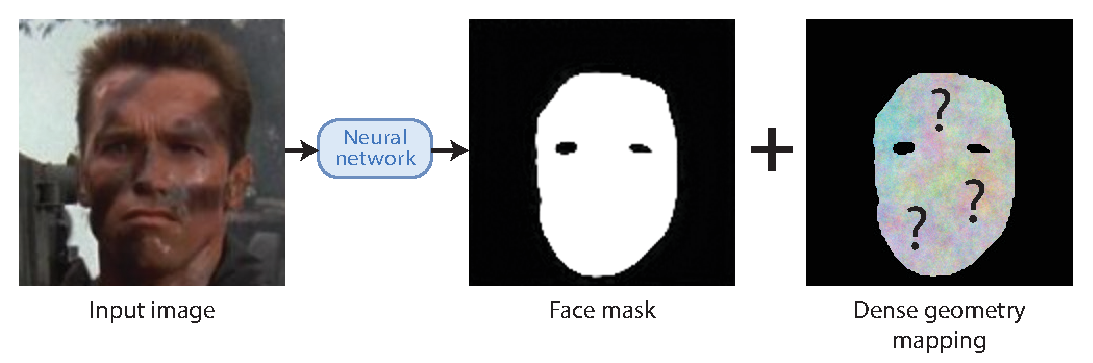
\includegraphics[width=\textwidth]{problem}
    \caption[Main research goal]{The main research goal visualized. A \acf{FCNN} is given a real-world human face image as an input, and the result should be the face segmented out of the background and densely filled with useful geometry information.}
    \label{fig:research_problem_1}
\end{figure}

\acp{CNN} have been shown to be able to extract relevant information from human faces, and the extension of \acp{CNN}, \acp{FCNN}, has been shown to be able to do dense pixel-to-pixel mappings in various situations. Could it be possible to train an \ac{FCNN} to extract human facial geometry information from an image and map it to another presentation densely pixel-per-pixel (see figure \ref{fig:research_problem_1})? An \ac{FCNN} can be trained in a supervised manner using a large number of densely annotated image pairs, but those are not readily available for real-world human faces. Could it be possible to generate these training pairs by rendering? Could the rendered data be non-realistic and still make it possible for the trained \ac{FCNN} to generalize to real-world images? What is the mapping that could be generated by rendering and that is possible for the \ac{FCNN} to learn? Could the rendered training dataset be extended using data augmentation to prevent overfitting and to enable occlusion detection?

\section{Research goals}

The main research goal of this thesis is to train a \acf{FCNN} using non-realistic synthetic data to do dense human facial geometry tracking on real-world images. If the network is given an image of a real human face as an input, the output should be a same sized image with the face segmented out of the background and filled with a useful dense geometry mapping. The main research goal is visualized in figure \ref{fig:research_problem_1}.

\newpage

This main goal can be divided into seven subgoals:

\begin{itemize}
    \item Design and implement a suitable network topology and a loss function using a Python-based deep learning framework, e.g., \textcite{cntk}. If the topology and loss functions are good enough, the network should produce non-blurry, sharply defined, results with a reasonable number of parameters.
    \item Design and implement a method to generate a large quantity of non-realistic synthetic training data in a reasonable amount of time. The dataset should be big enough and have a precise enough mapping that the training of the \ac{FCNN} is possible. Also, rendering a new dataset should take less than 24 hours.
    \item Make the network generalize well to real-world images of human faces. Even if the network is trained on completely non-realistic data, the network should be able to detect real-world faces and extract relevant geometry information from them.
    \item Make the feature detection of the network invariant to lighting, texturing, scaling and positioning. Even if the subject in the real-world image is under extreme conditions, the network should continue to output believable segmentation and geometry mapping.
    \item Enable the network to inpaint believable geometry under occlusions. If the face is, for example, partially occluded by sunglasses, the network should be able to detect them and generate geometry underneath.
    \item Implement geometry mapping visualizations and, in general, make the evaluation of results easy. It should be possible to see how well the generated geometry matches the real subject, and comparing results between different network versions should be effortless.
    \item Make the network generate temporally stable geometry mappings when applied to video. When looking at a video, the generated geometry should not flicker and jump around from frame to frame.
\end{itemize}

\section{Research scope}

The scope of this thesis includes the neural network design, synthetic data generation, data augmentation, training of the network, geometry mapping visualizations, and evaluation of the results. The facial geometry is identified in the canonical 2D parameterization. Because of time constraints, the extraction of 3D geometry from the parameterization has not been included.


\cleardoublepage
\chapter{Background and related work}

To give some background to our method this chapter first gives a brief overview of machine learning and neural networks. Then, a selection of face detection, recognition, and reconstruction methods are presented. More emphasis is given to facial reconstruction methods, especially those that have been developed recently and use neural networks and synthetic data in one way or another.

% Finally, selected parts of computer graphics theory are presented.

\section{Machine learning and neural networks}

If we have a parametric function $f(\bm{x};\bm{\theta}) = \bm{y}$, how should the parameters $\bm{\theta}$ be adjusted so that, with input $\bm{x}$, the output of the function matches $\bm{y}$ as closely as possible? Machine learning, and especially its most common form, supervised machine learning, can be used to solve this problem. In supervised learning, the parameters $\bm{\theta}$ are iteratively adjusted until the output of the function cannot be further made more accurate. To make these kinds of small adjustments, a number of training pairs $(\bm{x}_i,\bm{y}_i)$ are needed in addition to some metric that tells how well the function is performing. \cite{Goodfellow2016,LeCun2015}

The function performance can be measured by a separate loss function that tells how far the output of the function is from the desired values. In the case of fitting a simple line function to a collection of points, the loss function could be visualized as the sum of the distances of the points from the line. If the points lie exactly on the line, the loss becomes zero, and further away the points are from the line, the bigger the loss becomes. Especially with more complex functions, the loss could be visualized as a multi-dimensional hilly landscape. Lower values of the loss function are valleys, and higher values are hills. The lower it is possible to travel in this loss landscape, the better the function under optimization performs. With complex functions, the loss landscape has numerous valleys and hills. Even if it seems that the loss is now small, because you are at the bottom of a valley, it is very much possible that there exists another valley somewhere else that is even deeper and thus better. \cite{Goodfellow2016,LeCun2015}

To adjust the parameters of the function, an algorithm called gradient descent is used. The gradient of the loss function can be visualized as an arrow that, at any point in the loss landscape, points towards the direction of the greatest ascent. To travel towards lower loss function values, that is, towards the bottoms of the valleys, a step into the opposite direction of the gradient should be taken. When repeated enough many times, a loss function minimum is reached. The problem with gradient descent is that, after reaching a bottom of a valley, the algorithm cannot continue. This means that the optimization could get stuck into a local minimum even though much better minima would be available further away. \cite{Goodfellow2016,LeCun2015}

If a very accurate gradient is calculated using all the available training data, it is very much possible for the gradient descent algorithm to get stuck at a local minimum. The accurate gradient calculation is also time-consuming and usually needs the whole dataset to be kept in memory. This is not feasible for very large datasets. The \ac{SGD} algorithm solves this problem by calculating a less accurate gradient from a smaller, randomly selected, part of the training dataset. This small selection of training samples is called a minibatch. The more random gradient is faster to calculate, and because it is noisy, it will help the gradient descent algorithm to escape from local minima. \cite{Goodfellow2016,LeCun2015}

Instead of using just one function as the target of the optimization, a composite of multiple functions, a network, can also be used. These networks are usually called neural networks because the functional parts are loosely inspired by neuroscience. A neural network has an input layer, any number of hidden layers, and an output layer. The adjacent layers can be fully connected to each other with distinct weights for each connection, and the values that flow through the network can be modified with activation functions. The hidden layers are called so because the training data does not give any desired output for them. Instead, when trained, the network is free to come up with its internal representations. The training of a neural network like this is enabled by the backpropagation algorithm. For it to work, one requirement is that the functions that compose the network are differentiable. If this is the case, the gradient calculated at the output layer can be backpropagated through the network, and all the parameters of the network can be adjusted accordingly. \cite{Goodfellow2016,LeCun2015}

The machine learning algorithms used today are largely the same as in the 1980s. The massive increase of computing power, storage space, and memory amounts in recent years has enabled the training of networks that were previously thought very hard to train. The modern general processing \acp{GPU} have been instrumental in making the training process faster, as their architecture suits the task very well. Some other smaller developments, e.g., using the \ac{RELU} activation function, have also played their part in making the training of deeper networks easier. Modern neural networks can have tens of millions of parameters, and the networks can be very deep with tens, if not hundreds, of layers. Deep learning, the name given to this new era of machine learning, reflects this fact. A good example of the deep learning advantage is the application of deep neural networks by \textcite{Krizhevsky2012} in the 2012 ImageNet competition. Their results were impressive, almost halving the error rate compared to the best competitors. \cite{Goodfellow2016,LeCun2015}

The functions that the network is composed of can also perform filtering using convolutions. These kinds of networks are called \acfp{CNN}. Convolutions can be though as small filters that are slid over the larger underlying signal and that produce a new, modified, signal. Convolutions are especially well suited for processing images. One of the first applications of \acp{CNN} was a method to recognize handwritten digits, developed by \textcite{Lecun1998}. Many convolutions, with differing filter values, can be applied to the same image. This allows the extraction of different features from the image. The hierarchical nature of the \acp{CNN} means that, at the first layers, the extracted features are edges, and then continuing deeper inside the network the features become parts, and parts become objects. The structure of \acp{CNN} has been directly inspired by the concepts in visual neuroscience. \cite{Goodfellow2016,LeCun2015}

An ordinary \ac{CNN} usually has fully connected layers at the end and will produce a one-dimensional vector as the final output \cite{Lecun1998}. In \acfp{FCNN}, the fully connected part at the end is replaced by a convolutional upsampling part \cite{Long2015}. This means that, for \acp{FCNN}, both the inputs and outputs can be images. \acp{FCNN} have been successfully used for dense image semantic segmentation. Semantic segmentation means understanding the image at the pixel level, i.e., giving each pixel of the input image a meaningful class \cite{Long2015,Ronneberger2015}. The training of \acp{FCNN} has been made easier with the introduction of the concept of skip connections. Skip connections connect the downsampling and upsampling parts of the \ac{FCNN} directly. Skip connections have been shown to help gradients propagate from the output towards the input side of the network, transfer high-frequency detail from the input side to output side, and help to avoid singularities in the loss landscape \cite{Ronneberger2015,Orhan2017,Goodfellow2016}.

Designing and training the neural networks, especially the deep ones, would be very time-consuming if the training code had to be reimplemented at low-level with every design iteration. To get fast enough training speeds, using \acp{GPU} is necessary. The training code has to be executable on \acp{GPU}, and efficient transfer of training data to the \acp{GPU} needs to be implemented. To help make the neural network design process, code generation for the \acp{GPU}, data transfer to the \acp{GPU}, and the training process easier, numerous software frameworks have been developed in recent years. Good examples of these software frameworks are \textcite{cntk}, \textcite{tensorflow}, and \textcite{pytorch}. With these frameworks, the neural network can be designed at high-level with the Python scripting language. Changes to the network topology can be made easily, and the framework will take care of converting the high-level network description into optimized low-level code that is ready to be run on \acp{GPU}. \cite{cntk,tensorflow,pytorch}

\section{Face detection and reconstruction}

The techniques for processing human faces in images are broadly classified into three categories by \textcite{Datta2015}: face detection, face recognition, and face reconstruction. Face detection tells us if there exists a human face in an image in the first place, and can give the approximate location and size of the face. Face recognition goes a step further as it can identify the actual person in the image. Face reconstruction does not necessarily have anything to do with identification but rather finding out the underlying facial geometry, i.e., the facial shape, of the human pictured.

\begin{figure}
    \centering
    \subfloat[\cite{Sakai1972}]{\label{fig:face_detection_1a}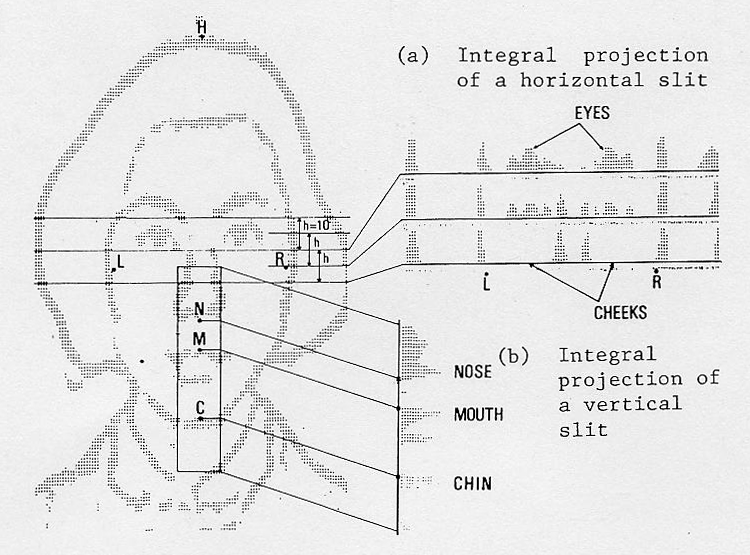
\includegraphics[height=.3\textwidth]{takeo}}\qquad\qquad
    \subfloat[]{\label{fig:face_detection_1b}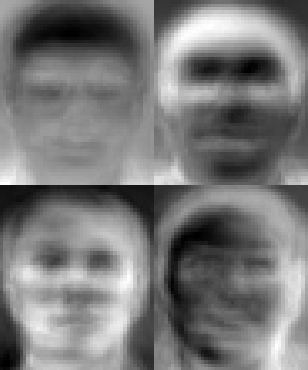
\includegraphics[height=.3\textwidth]{eigenfaces}}
    \caption[Face detection 1]{One of the first face detection systems was developed in the early 1970s by \textcite{Sakai1972}. Their algorithm was based on analyzing slices of a binary image of the head as shown in \protect\subref{fig:face_detection_1a}. Face recognition based on eigenfaces, as proposed by \textcite{Turk1991}, was one of the first commercially viable methods for face recognition. Visualizations of eigenfaces are shown in \protect\subref{fig:face_detection_1b} (Copyright of AT\&T Laboratories Cambridge).}
    \label{fig:face_detection_1}
\end{figure}

One of the first automated face detection systems was developed in the early 1970s by \textcite{Sakai1972}. The input was a 5-bit grayscale image with a resolution of 140x208. The image was processed with an edge detecting filter and then thresholded to obtain a binary image containing contours of the face. See figure \ref{fig:face_detection_1a} for an example. The binary image was then scanned slice-by-slice from top to bottom. Each slice was analyzed while an elaborate state machine kept track whether the image contained a human or not. The face had to be centered in the image and could have only a small amount of tilt in any direction. This method did not work at all if the person in the image had glasses or a beard.

The method of using eigenfaces for recognizing humans from pictures was introduced by \textcite{Turk1991} in 1991. It was one of the first accurate and fast enough methods to be used commercially. The method captured the relevant variation in a collection of facial images, that is, the principal components of the distribution, into eigenvectors. The eigenvectors can be visualized as ghostly faces, eigenfaces, as is shown in figure \ref{fig:face_detection_1b}. Any picture of a human face could then be deconstructed into a linear combination of eigenvectors, and inversely, reconstructed with the same linear combination of the same eigenvectors. The face recognition could be done by comparing the weights of the linear combinations as the weights would be similar between two images of the same person.

\begin{figure}
    \centering
    \subfloat[\cite{Viola2001}]{\label{fig:face_detection_2a}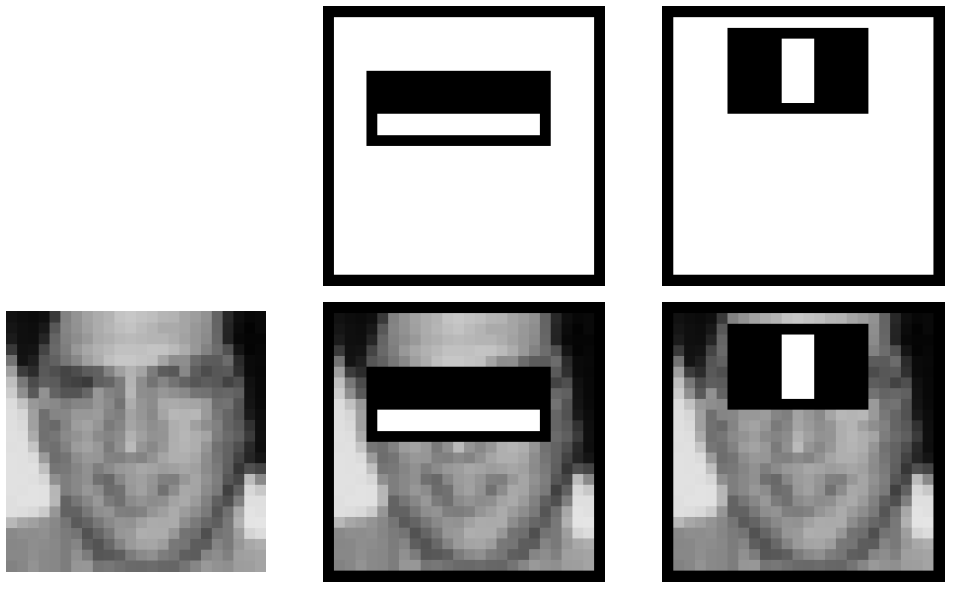
\includegraphics[height=.28\textwidth]{viola}}\hfill
    \subfloat[ \cite{Osadchy2007}]{\label{fig:face_detection_2b}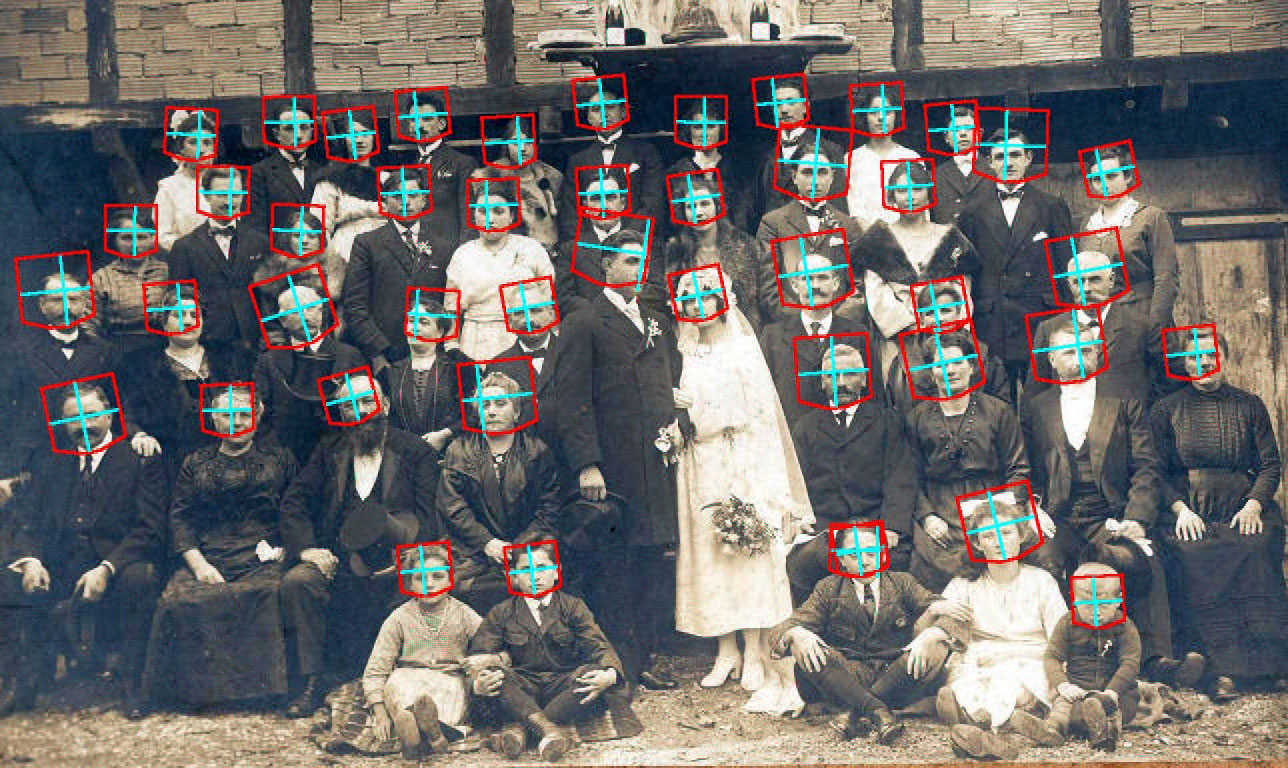
\includegraphics[height=.28\textwidth]{osadchy}}
    \caption[Face detection 2]{Face detection speed was greatly increased by a method introduced by \textcite{Viola2001}. The method was based on fast evaluation of rectangular filters and machine learning. Some filters are visualized in \protect\subref{fig:face_detection_2a}. Convolutional neural networks were used by \textcite{Osadchy2007} for fast face detection and pose estimation. \protect\subref{fig:face_detection_2b} shows how the algorithm performed on a somewhat difficult image.}
    \label{fig:face_detection_2}
\end{figure}

The speed of detecting faces and generating the bounding boxes around them was dramatically improved by \textcite{Viola2001} in 2001. Their proposed method was based on the idea of the integral image, rectangular feature filters, and machine learning. The integral image, or summed area tables, was an intermediate representation of the image that allowed rapid summation of pixels in arbitrary rectangular areas. The rectangular feature filters are illustrated in figure \ref{fig:face_detection_2a}. The filter calculated the sum of the pixels in the white area which was then subtracted from the sum of the black area. The filter could thus find intensity variations between arbitrary rectangular areas rapidly. Hundreds of thousands of possible combinations of these filters existed for a 24x24 pixel detection window, and machine learning was used to select few thousand of the most relevant filters for human face detection. Applying the resulting combination of filters to images was fast, and faces could be detected and tracked near real-time with contemporary hardware.

In 2007, \textcite{Osadchy2007} published a novel method for simultaneously detecting faces and estimating their poses in real-time using convolutional neural networks. Figure \ref{fig:face_detection_2b} shows how the network was able to detect multiple faces in one image including their yaw from left to right and in-plane rotation. Their network topology was similar to the one used by \textcite{Lecun1998} in 1998 to recognize hand-written digits. The training data consisted of real human faces which were manually annotated with the pose data. The method could do face detection and pose estimation at the same time quicker and more accurately than previous methods that did the tasks separately.

\begin{figure}
    \centering
    \subfloat[\cite{Blanz1999}]{\label{fig:face_reconstruction_1a}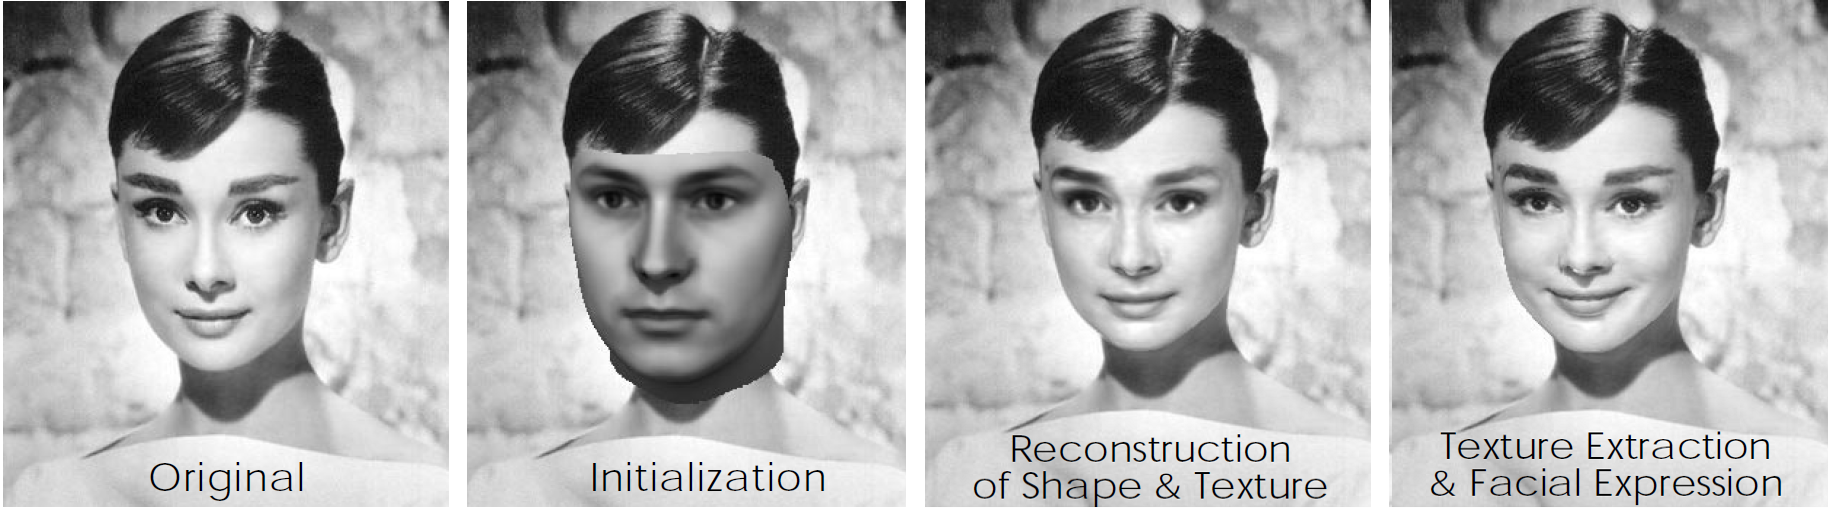
\includegraphics[height=.2\textwidth]{blanz}}
    
    \subfloat[\cite{Richardson2016a}]{\label{fig:face_reconstruction_1b}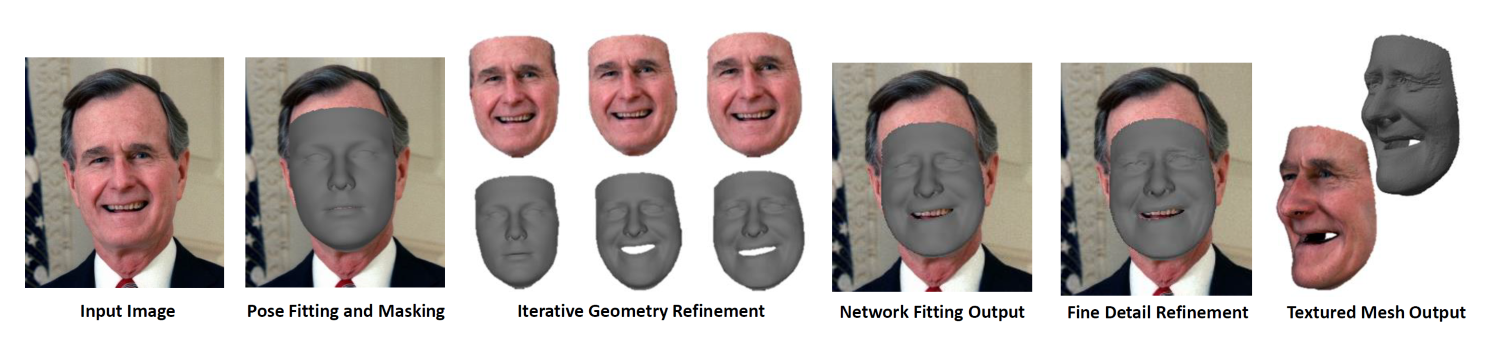
\includegraphics[width=\textwidth]{richardson1}}
    \caption[Face reconstruction 1]{Facial geometry and texture reconstruction using a 3D morphable model was proposed by \textcite{Blanz1999}. The steps of their algorithm are shown in \protect\subref{fig:face_reconstruction_1a}. \textcite{Richardson2016a} used a \ac{CNN} and an iteration process to fit the morphable model to the input image. The steps are shown in \protect\subref{fig:face_reconstruction_1b}.}
    \label{fig:face_reconstruction_1}
\end{figure}

In 1999, \textcite{Blanz1999} introduced a new technique to reconstruct human facial geometry from a single image using a 3D morphable face model. They started by scanning hundreds of real human faces with a 3D laser scanner. The scan produced accurate vertex positions and colors. The generated 3D face models were processed so that they all came into full correspondence with each other. Using \ac{PCA} decomposition, an average face model and a set of basis face vectors were created. \ac{PCA} was also done for the vertex color data. This allowed a parametric creation of 3D face models and their textures. The process of reconstructing the facial geometry from a single image started with a coarse manual alignment of the average face model over the image. An analysis-by-synthesis loop was then repeated where the face model was rendered over the image, and the factors of the principal components were adjusted until an optimization minimum was reached. Finally, additional detailed facial texture information was extracted from the image as the color \ac{PCA} components did not contain enough high-resolution data. Steps of this process are shown in figure \ref{fig:face_reconstruction_1a}.

More recently, in 2016, \textcite{Richardson2016a} proposed a method to extract 3D morphable model parameters from real-world images using a \ac{CNN}. The steps of their algorithm are visualized in figure \ref{fig:face_reconstruction_1b}. They started by aligning the average morphable face model over the image using another posing algorithm. The face was segmented out of the background and fed to the \ac{CNN} along with a rendered version of the current morphable face model. The \ac{CNN} was trained to output a correction term to the morphable model parameters to make the rendered face model match the segmented real face image better. The face model rendering and parameter correction calculation were repeated iteratively multiple times to increase the quality of the reconstruction. The \ac{CNN} was completely trained on synthetic data generated using the 3D morphable face model. Because fine facial details could not be extracted using this method, they were later captured with a separate shape-from-shading algorithm.

\textcite{Richardson2016} improved their previous method of \cite{Richardson2016a}. The problem with their previous method was that it needed separate initialization of the average face model over the input image and that the method could not extract fine details without an external algorithm. The improved algorithm could do both in one go using two connected networks, a \ac{CNN} and an \ac{FCNN}. The \ac{CNN} was applied iteratively to the input image and a coarse geometry using a 3D morphable model was recovered. A depth map was generated from this model, and the map was fed to the \ac{FCNN} along with the input image. The \ac{FCNN} was trained to do fine detail reconstruction, i.e., shape-from-shading, within the depth map in one shot without iteration. The \ac{CNN} was trained in a supervised manner with synthetic data rendered using the 3D morphable model, and the \ac{FCNN} was trained in an unsupervised manner using real-world images.

\textcite{Kim2017} introduced a method that could estimate a wide variety of 3D morphable model parameters from a real-world image in a single shot using a \ac{CNN}. The estimated parameters included facial pose, facial shape, facial expression, skin reflectance, and scene illumination. No iteration was needed to refine the results. Before feeding the real-world images to the network, their variety was reduced by segmenting the faces out of the backgrounds using facial landmark detection. The network was trained exclusively on synthetic training data derived from the 3D morphable model. To get the parameter distributions of the synthetic training data to better model the real-world distributions, a novel breeding method was introduced that used real-world facial images to update the training set. A network trained with the breeding outperformed a network trained only on synthetic data.

\textcite{Tewari2017} were able to train an autoencoder \ac{CNN} completely unsupervised using only real-world images. No separately generated synthetic data was used. The \ac{CNN} was able to extract 3D morphable model parameters including facial pose, facial shape, facial expression, skin reflectance, and scene illumination in a single iteration. The method relied on a novel analytical and differentiable decoder layer that used the morphable model parameters to reconstruct the input image. It was possible to train the network in an unsupervised manner because the loss could be backpropagated through the decoder layer. With a method like this, the real-world distribution of the morphable model parameters could be captured the best, and the network could generalize well to real-world images.

\begin{figure}
    \centering
    \subfloat[\cite{Sela2017}]{\label{fig:face_reconstruction_2a}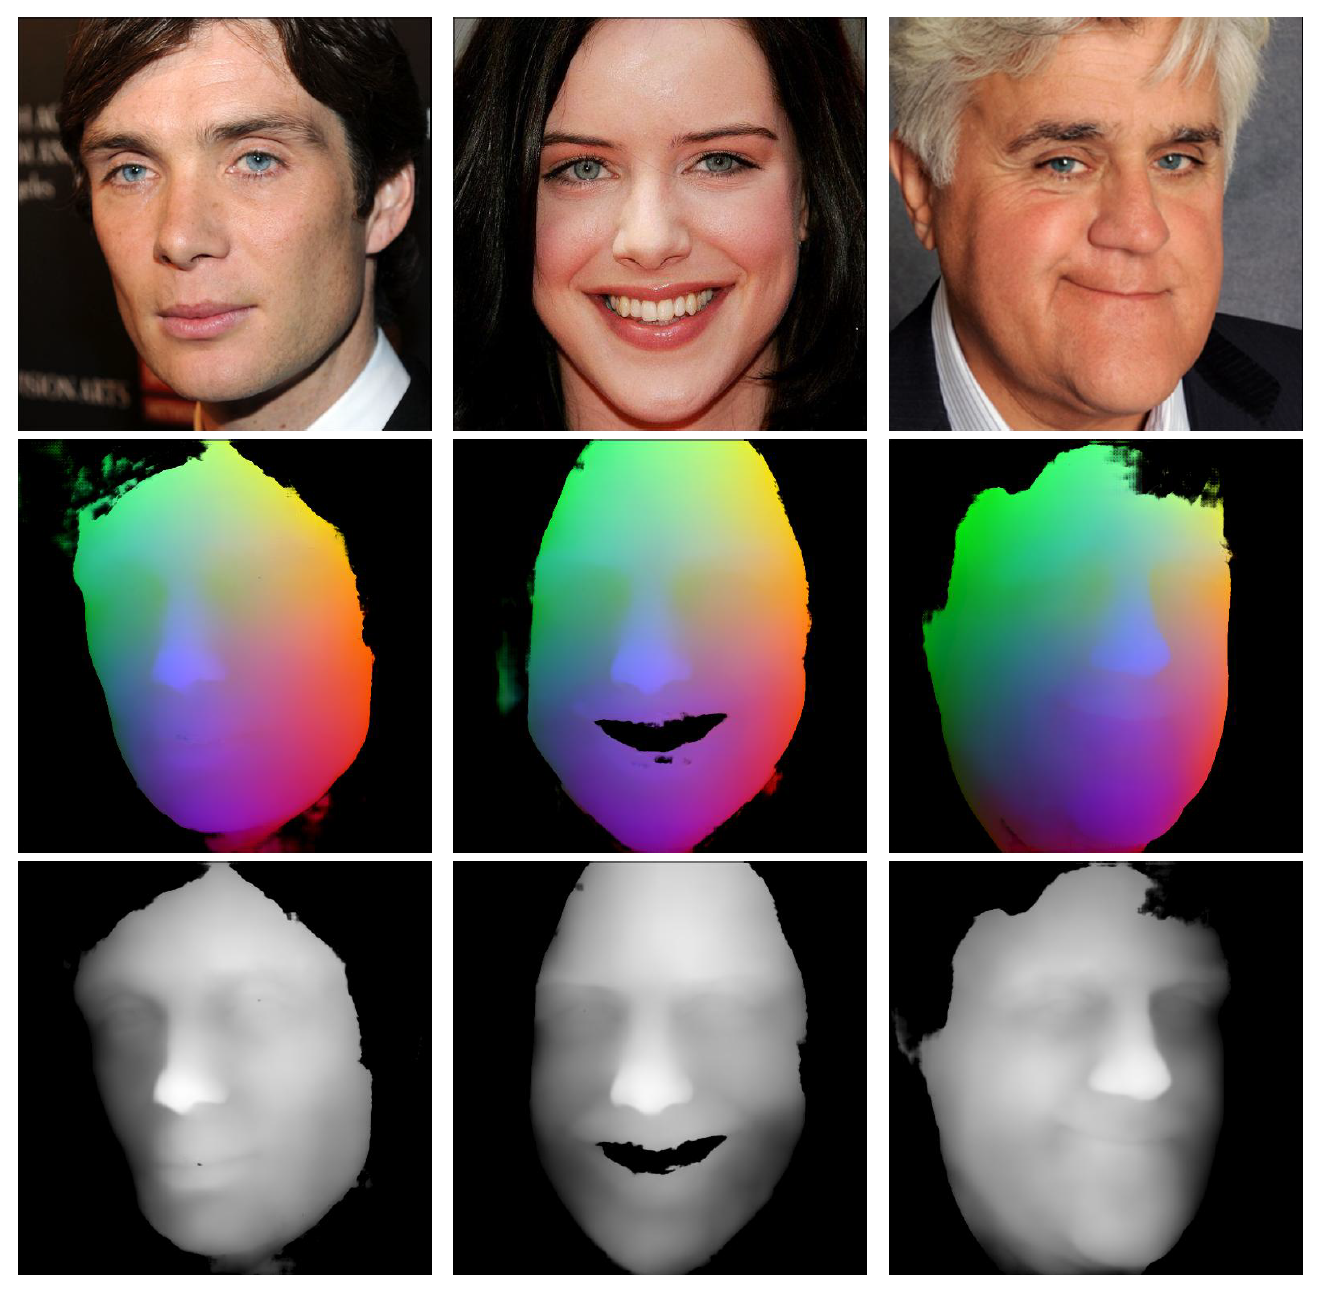
\includegraphics[height=.3\textwidth]{sela1}}\qquad\qquad
    \subfloat[\cite{Guler2016}]{\label{fig:face_reconstruction_2b}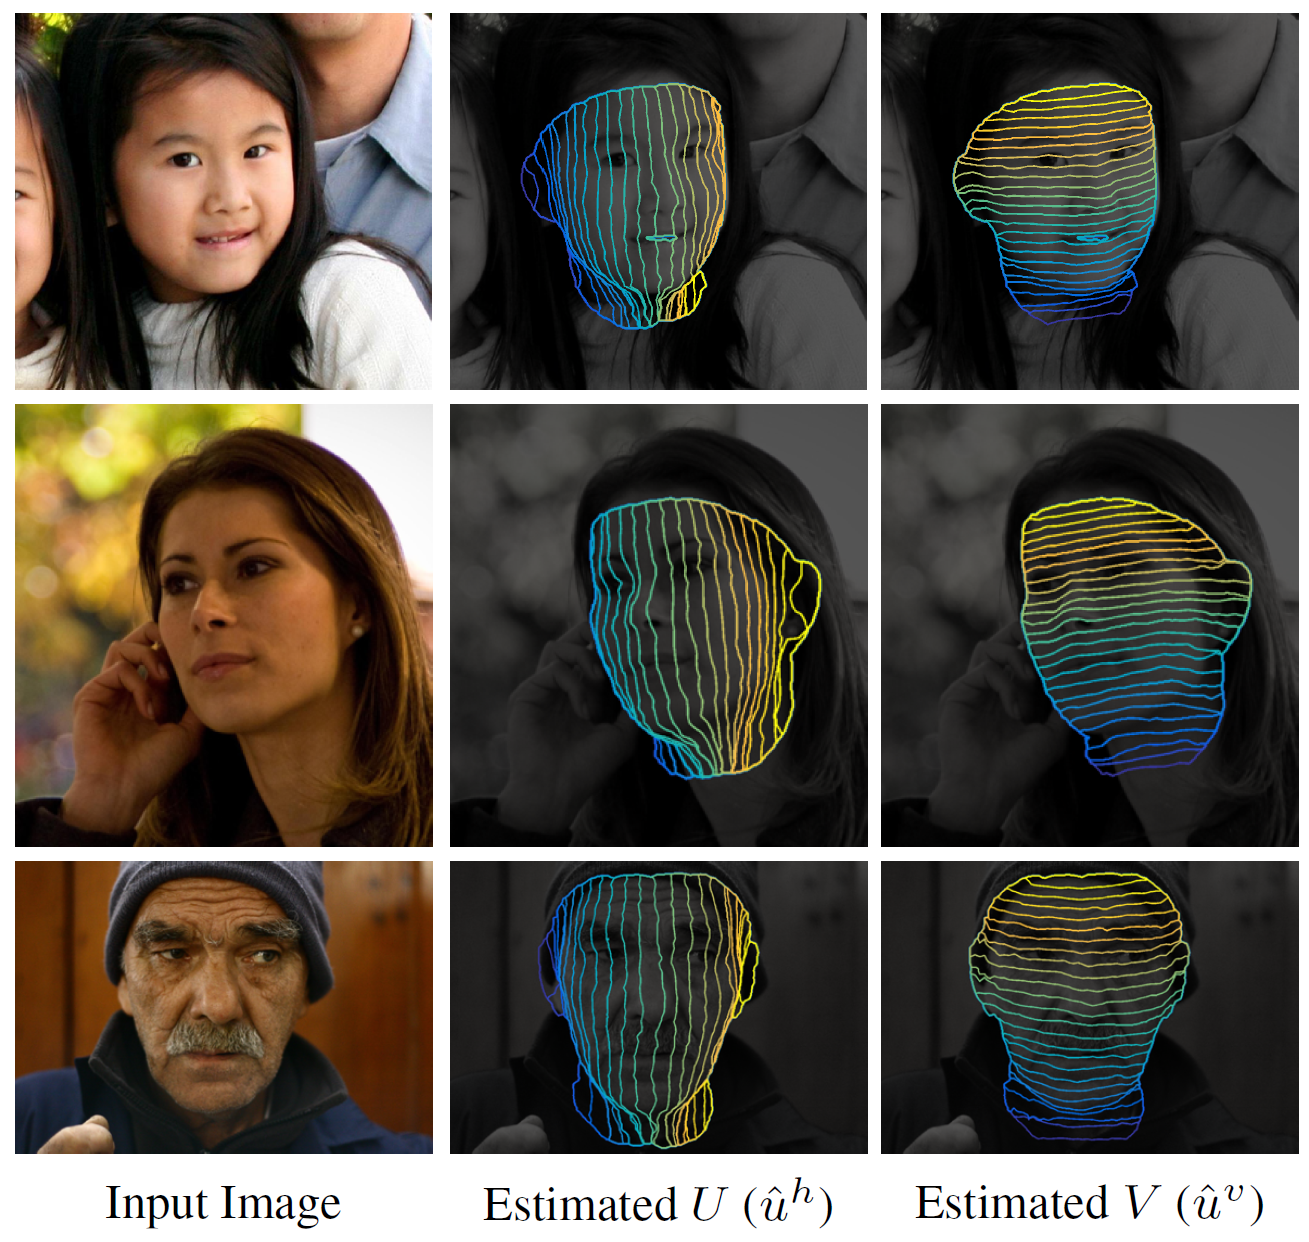
\includegraphics[height=.3\textwidth]{guler1}}
    
    \subfloat[\cite{Yu2017}]{\label{fig:face_reconstruction_2c}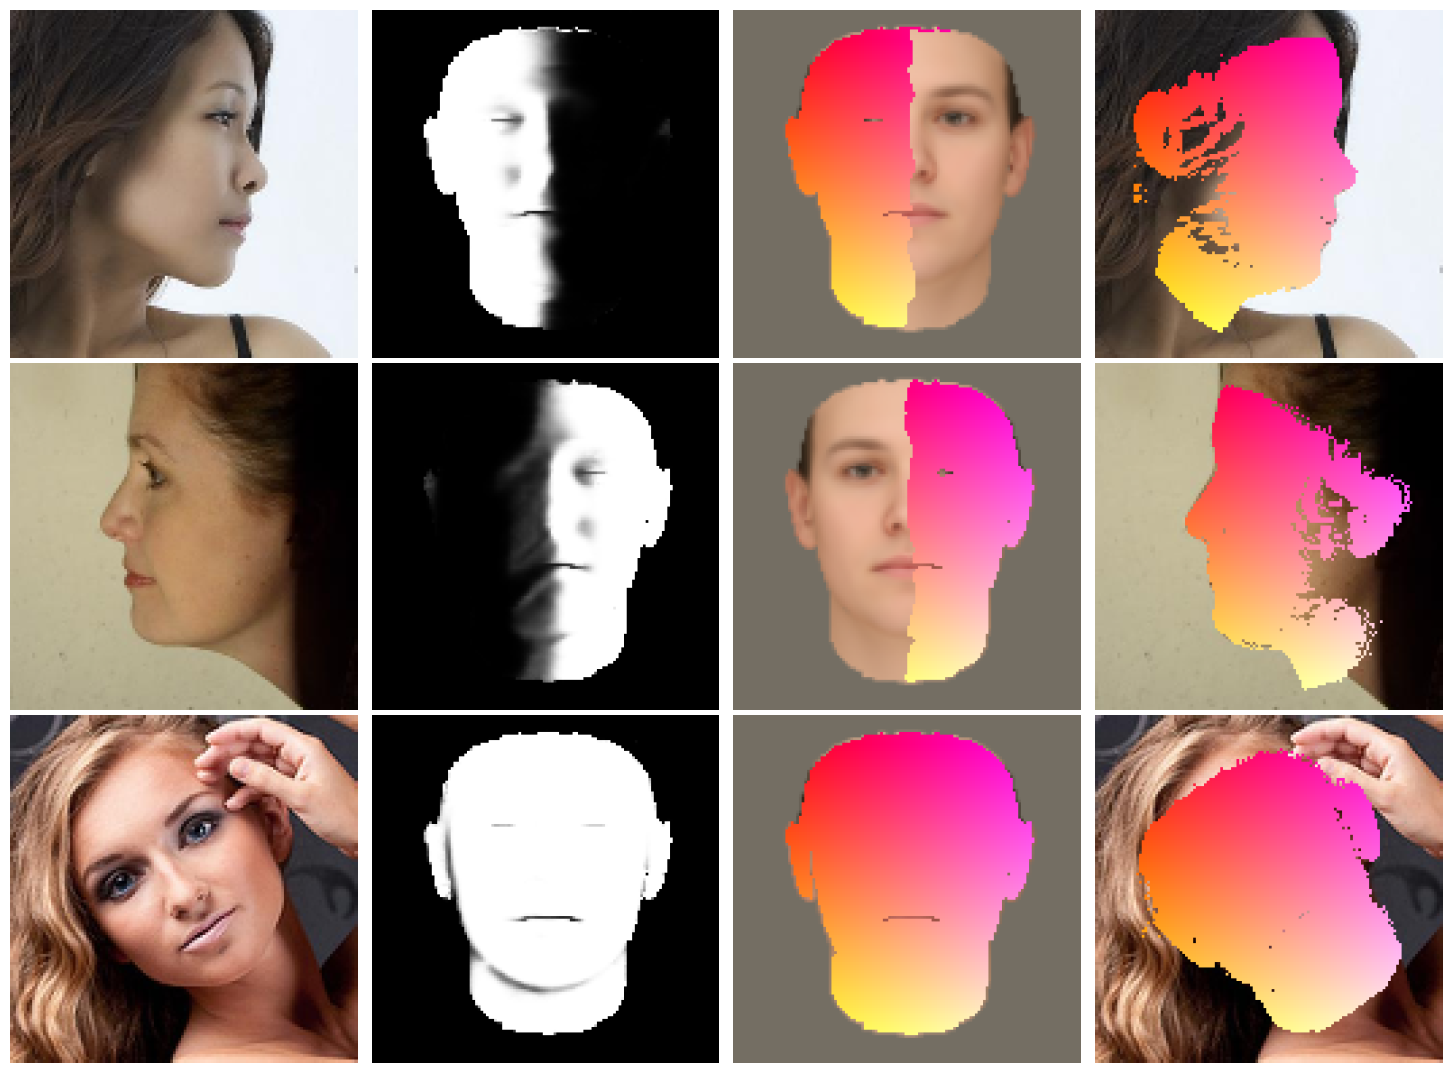
\includegraphics[height=.3\textwidth]{yu1}}
    \caption[Face reconstruction 2]{The method of \textcite{Sela2017} generated dense correspondence and depth map images. Their results are shown in \protect\subref{fig:face_reconstruction_2a}. \textcite{Guler2016} generated dense correspondences using quantized regression which resulted in outputs shown in \protect\subref{fig:face_reconstruction_2b}. \textcite{Yu2017} proposed a method that could estimate dense 2D pixel flow between the input image and a front-facing template mesh. Visualization of their method is shown in \protect\subref{fig:face_reconstruction_2c}.}
    \label{fig:face_reconstruction_2}
\end{figure}

After the work on this thesis had started, multiple papers were published that had similar ideas regarding \acp{CNN} and dense geometry generation. \textcite{Sela2017} proposed an \ac{FCNN} that could map a real-world human face image to a dense correspondence image and a dense depth map image. Examples of these images are shown in figure \ref{fig:face_reconstruction_2a}. In contrast to most of the previously mentioned methods, this method did not use a 3D morphable model in the reconstruction process. The correspondence and depth map images were then used with a separate algorithm to extract the 3D mesh of the face. The network was trained with synthetic data with a wide range of facial shapes, facial poses, facial materials, lighting conditions, and background textures. A surprising result was that even though the synthetic data was created with a limited generative model, the network could generalize beyond the limited scope of the training material.

\textcite{Guler2016} trained an \ac{FCNN} to estimate dense correspondences between image pixels and a 3D template mesh projected onto a 2D deformation-free space, or in other words, a UV space. Their approach was very similar to ours, but instead of plain regression, they used quantized regression. The mappings generated by this method are illustrated in figure \ref{fig:face_reconstruction_2b}. The training dataset was generated from real-world images that had existing facial landmark annotations. The dataset generation was done by first fitting the 3D template mesh over the image using the landmarks and then rasterizing the mesh using colors representing locations in the deformation-free space.

\textcite{Yu2017} used an \ac{FCNN} to generate dense facial correspondences between the input image and a 3D morphable face model. Two images were generated from the input image: a 2D flow image and a matchability mask image. The 2D flow image estimated the flow between the input image pixels and a synthetic rendering of an average frontal face. The matchability image indicated which correspondences were valid inside the average face. These images are visualized in figure \ref{fig:face_reconstruction_2c}. In the beginning, the network was trained with synthetic data generated from a 3D morphable model. Later, the network was refined using annotated real-world images. Simple rectangular occlusions were also added to the training data which made the model more robust against obstructions over the faces.

\begin{figure}
    \centering
    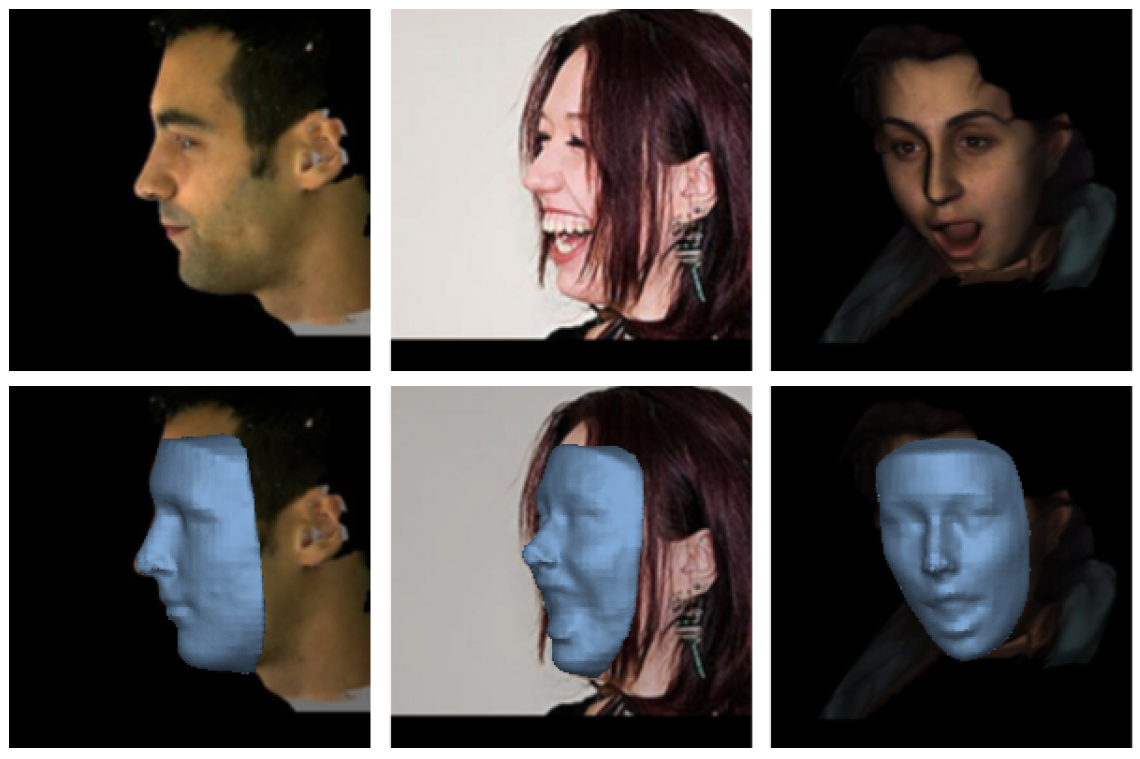
\includegraphics[height=.4\textwidth]{jackson1}
    \caption[Face reconstruction 3]{Results of the method proposed by \textcite{Jackson2017}. They used \acp{FCNN} to regress from the input image into a 3D volume directly.}
    \label{fig:face_reconstruction_3}
\end{figure}

In late 2017, \textcite{Jackson2017} published a novel method that used \acp{FCNN} for direct 2D-to-3D facial geometry reconstruction. No intermediate fitting steps were used. The training dataset consisted of real-world images and corresponding 3D binary volumes that modeled the faces in the input images. Inside the volume, if a voxel was inside the face, it was given a value of 1, and 0 otherwise. The 3D binary volumes were created using a 3D morphable model that was already fitted to the input images. The actual 3D facial geometry was recovered by generating the iso-surface of the regressed binary volume. Results of this method are shown in figure \ref{fig:face_reconstruction_3}.

\iffalse

\section{Computer graphics and rendering}

Computer graphics theory is a vast subject area. The relevant parts of it, for this thesis, are 3D mesh representation, texture mapping, surface reflectance models (\acsp{BRDF}), the light transport equation, path tracing, and antialiasing.

\begin{gather}
L_o(p, \omega_o) = L_e(p, \omega_o) + \int_\Omega f(p, \omega_o, \omega_i) L_i(p, \omega_i) |cos\theta_i| d\omega_i
\end{gather}

\begin{Verbatim}
- how 3D meshes are composed of triangles
- triangles have vertices that have 3D world coordinates and 2D UV coordinates
- UV coordinates are used for texture mapping
- rendering can be performed by shooting rays from the camera
- realistic images can be generated by solving the lighting equation
- lighting equation can be solved using path tracing
- light bouncing determined by surface reflectance models (BRDFs)
- reflectance models (BRDFs)
- smoothing edges using antialiasing
\end{Verbatim}

\begin{figure}[h]
    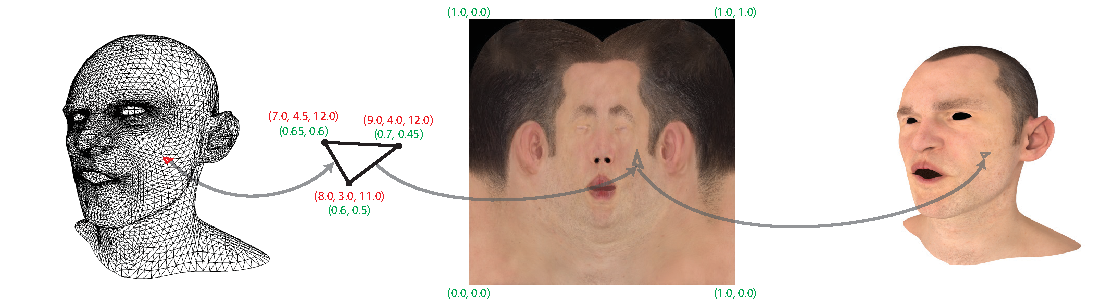
\includegraphics[width=\textwidth]{tex-mapping}
    \caption[Texture mapping]{An illustration of the texture mapping process. A 3D mesh consists of triangles. Each vertex of a triangle usually has at least a 3D world coordinate (red) and a 2D UV coordinate (green). UV coordinates map the triangle onto the 2D UV space of the texture. The color from the texture can be applied to the triangle when rendering.}
    \label{fig:tex_mapping_1}
\end{figure}

\fi

\cleardoublepage
\chapter{Our method}

A synthetic 3D model has a canonical, continuous, and dense 2D parameterization which is not dependent the 3D model pose or deformation. Pose means the translation and rotation of the model, and deformation means the independent movement of the model vertices. We used the 3D model to render large quantities of randomized, deformed, and non-realistic training data. The training data consisted of randomized facial images and corresponding 2D parameterization images. Using this data, we trained a neural network to detect faces from images and to identify the pixels inside the faces with the 2D parameterization. This gave a 2D correspondence between the face pixels and the 3D model.

This chapter goes into the details of our method, and the chapter is divided into sections as follows:

\begin{itemize}
    \item Section \ref{sec:general_workflow}, general workflow, describes the repeated high-level work that was needed to iteratively improve the results.
    \item Section \ref{sec:uv_color_mapping}, UV color mapping, explains how we used the 2D parameterization of the head model for the geometry mapping.
    \item Section \ref{sec:syn_data_gen}, synthetic data generation, explains the details necessary to create a diverse enough training dataset.
    \item Section \ref{sec:net_design}, neural network design, shows the final topology of the network and the particular features of its layers.
    \item Section \ref{sec:loss_func}, loss function design, illustrates how the training sample flowed through the network and how the final loss value was calculated from the resulting images.
    \item Section \ref{sec:data_aug}, data augmentation process, details every augmentation method we used to increase the effective size of the training dataset, and especially how the occlusion augmentations were created.
    \item Section \ref{sec:training_process}, training process, presents the software architecture used for the training.
    \item Section \ref{sec:viz_methods}, visualization methods, details all the techniques we used to generate evaluation images from the network outputs.
    \item Section \ref{sec:results_eval}, results evaluation, explains the technical details behind managing the evaluation and inspection of a large number of training runs and result images.
\end{itemize}

\section{General workflow}
\label{sec:general_workflow}

Figure \ref{fig:workflow_1} depicts the general workflow of our method from a higher level. We started by editing the head model and associated materials in the \textcite{blender} 3D computer graphics toolset. After having adjusted rendering parameters, a test rendering was executed on the local computer. This usually took about one hour and in the end generated a large collage with hundreds of renderings combined. Using this collage, we then determined if further rendering adjustments were necessary. If they were, this adjust-render-evaluate method was repeated until the renderings looked satisfactory.

\begin{figure}
    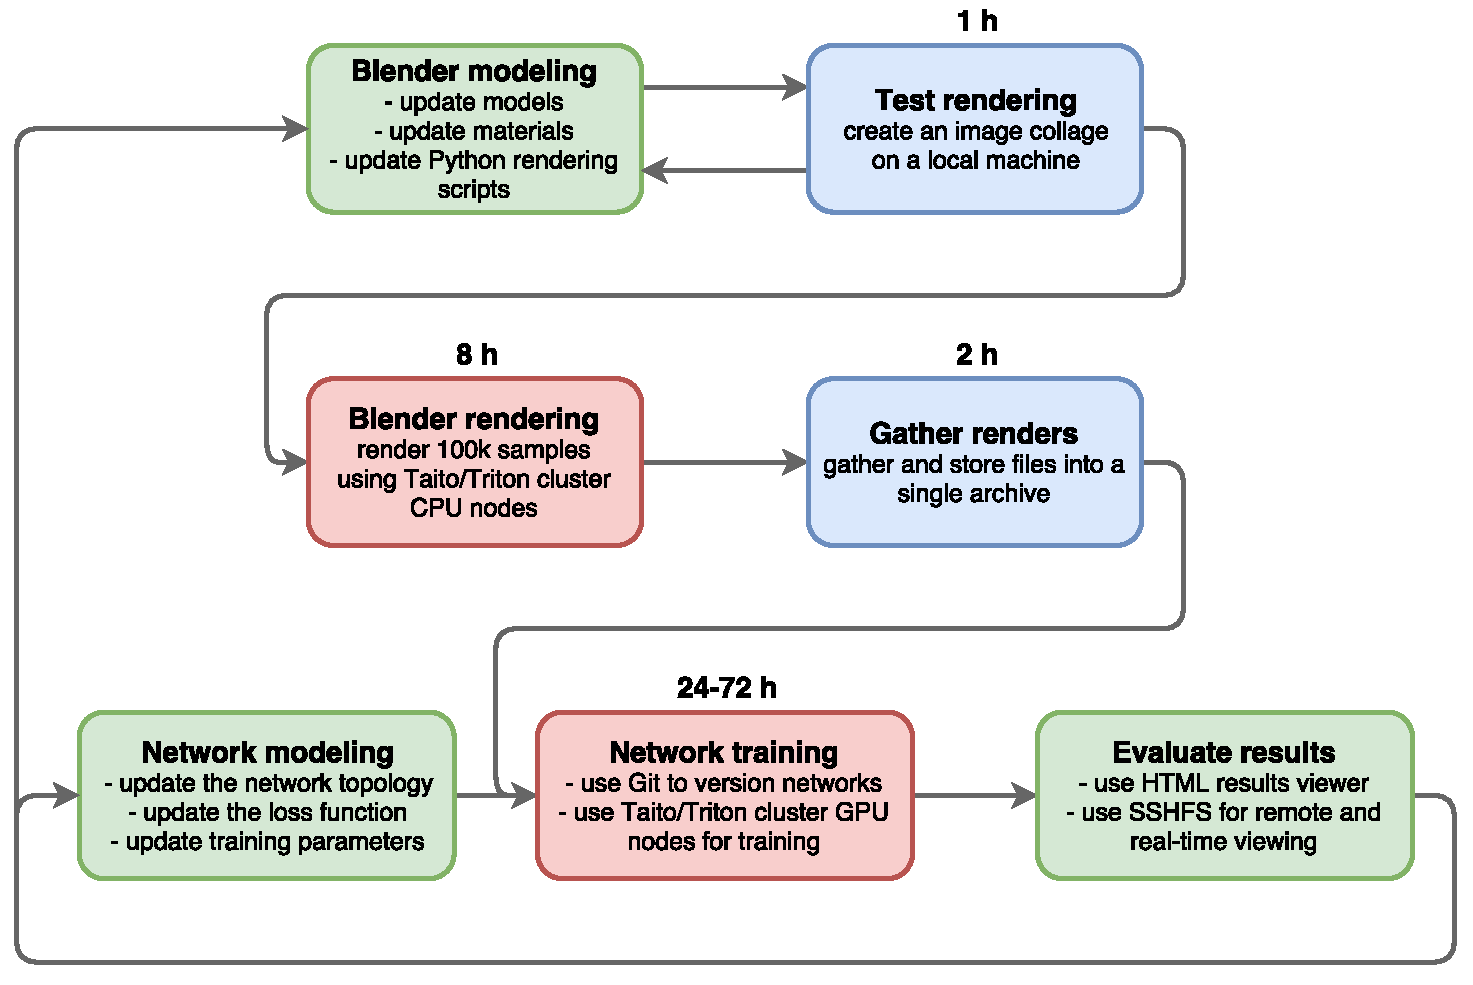
\includegraphics[width=\textwidth]{workflow}
    \caption[Research workflow]{Overview of our research workflow. Green boxes mean manual work that did not have an exact duration. Blue boxes mean small-scale non-parallel jobs. Red boxes mean massively parallel and long-running jobs on either the \ac{CPU} or \ac{GPU} nodes in the Aalto Triton or \ac{CSC} Taito computing clusters.}
    \label{fig:workflow_1}
\end{figure}

Updated rendering related files and scripts were then uploaded to the Aalto Triton or \ac{CSC} Taito computing clusters. There, a massively parallel rendering job was launched that generated 300 000 individual rendered images. The job took on average eight hours to finish. This big set of files was then gathered together and compressed into a single archive, taking over 10 gigabytes of storage space.

While the rendering was underway, we manually tuned the neural network parameters. The validity of the changes was tested on a local computer using quick test runs. We created up to 20 different training configurations where usually a single change was made to either network, loss, or augmentation parameters. After the training dataset generation had finished, we sent it together with 20 different training jobs to the \ac{GPU} nodes in the computing cluster.

After the models had been under training for a maximum of three days, we started to evaluate the results. The evaluation was done by mounting the result directory to a local computer using \ac{SSHFS} and then looking at the generated evaluation images using the custom-made browser-based viewer. We compared the results from all the 20 different jobs visually and by using some simple evaluation metrics. After we had come to conclusions with the current results, we started the process from the beginning by going back to updating the network and rendering models. In the end, this process was repeated about 15 times which means that around 300 24--72 hour training runs were performed.

\section{UV color mapping}
\label{sec:uv_color_mapping}

\begin{figure}[h]
    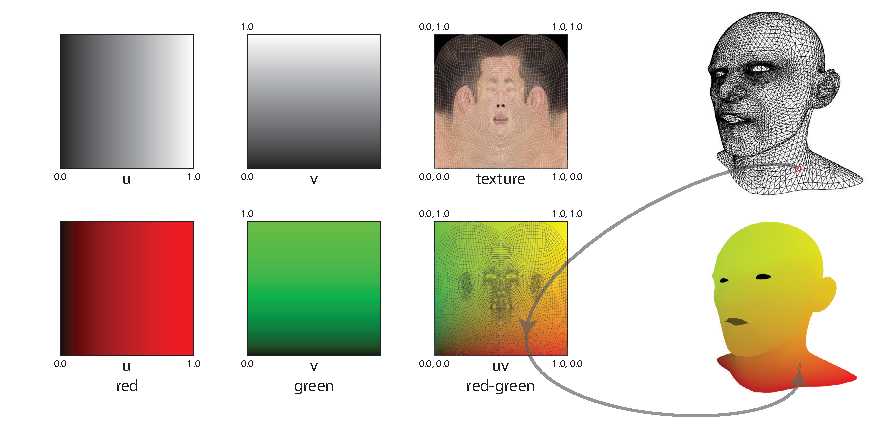
\includegraphics[width=\textwidth]{uv-color-mapping}
    \caption[UV color mapping]{UV color mapping. Same idea as in texture mapping but the texture is replaced by the procedural color representation of the UV coordinates. The 3D triangle mesh is ''opened up`` and flattened to the 2D UV space so that the triangles do not overlap.}
    \label{fig:uv_color_mapping_1}
\end{figure}

The key insight to our method is understanding the UV color mapping we used. Figure \ref{fig:uv_color_mapping_1} illustrates this idea. A 3D model consists of triangles, and each triangle has three vertices. These vertices each have at least two attributes: a 3D world position and a 2D UV coordinate. The position can have any arbitrary values, but the UV coordinate is constrained to values between 0.0 and 1.0. It could be thought that the 2D UV values are real-valued positions on a square whose side length is 1.0. When a 3D model is created, its UV mapping is generated at the same time automatically with some manual tuning afterward. The UV map generation can be visualized as opening the 3D model up and then warping and flattening the triangles onto the 2D UV square. The flattening is done so that the triangles do not overlap in the UV space, that is, each triangle is mapped to a unique area. After the UV mapping has been done, it does not change even if the 3D world positions of the model vertices are changed. The change could be caused by, for example, expression animation or by applying scaling or deformation operations to the 3D model. Figure \ref{fig:uv_color_mapping_1} illustrates the UV dimensions both in grayscale and with color; red for the U dimension and green for the V dimension. If these separate color channels were combined, it would result in a color gradient shown in the red-green square. The color choice has been arbitrary; it affects only on the visualizations of the results.

Usually, the UV mapping is used to texture the 3D model using textures like one in the texture square of figure \ref{fig:uv_color_mapping_1}. We replaced this normal texture with the red-green-yellow gradient texture generated procedurally straight from the UV coordinates. This resulted in the red-green-yellow renders of heads as seen in, for example, figure \ref{fig:head_final_triplet_collage_1}. Looking at a render like that, each pixel of the head tells precisely where that pixel belongs to in the UV space. Now, if we can generate this same UV color mapping from an arbitrary face image, we can then use the mapping to sample textures, create own visualizations using static or procedural textures, swap faces between two people, or recreate the 3D mesh of the face.

Many corresponding input and UV images can be rendered using just one head model while deforming it in many ways. Even if the appearance the model changed, the UV mapping would stay the same. These input and UV image pairs can then be used to train a neural network to do the mapping. The network can become invariant to facial geometry changes and would be able to map very different facial geometries to the same underlying UV mapping.

\section{Synthetic data generation}
\label{sec:syn_data_gen}

For generating the images in the training dataset, we decided to use \textcite{blender}. The choice was quite easy, as Blender is free and open source, and it has comparable features to commercial 3D modeling software. In addition, Blender comes with the Cycles rendering engine which has all the features we needed. We could use the nodes material system to design arbitrary materials and output resulting renders in multiple file formats. Blender is heavily based on the Python scripting language, and that allowed broad access to the internals of the program with the use of external scripts. This meant that we could completely automate and randomize the rendering process from start to finish. Finally, blender supports Linux and running from the command line without opening a \ac{GUI}, which meant the rendering of a lot of images could be parallelized on a computing cluster.

\begin{figure}
    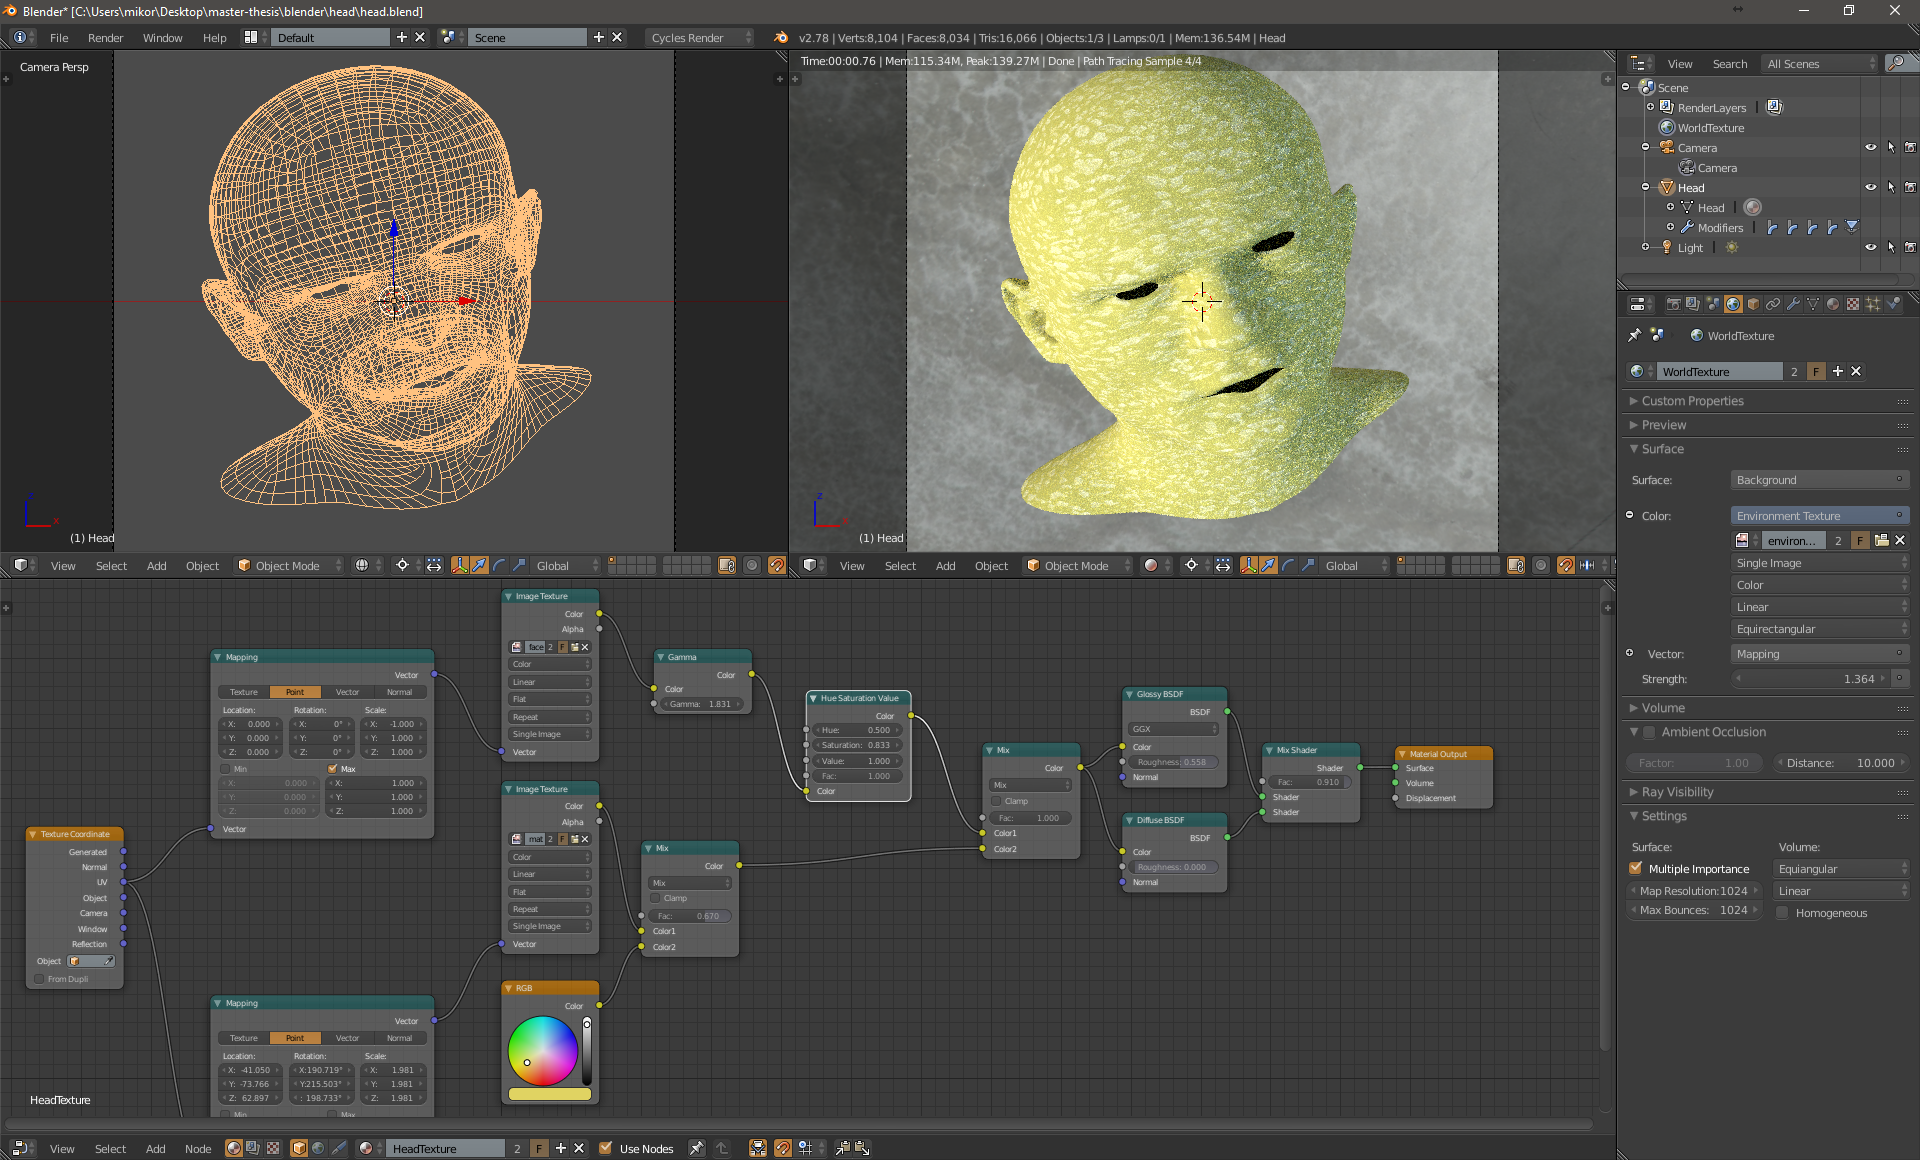
\includegraphics[width=\textwidth]{blender_edit_view}
    \caption[Blender modeling session]{A Blender modeling session. On the top left is the wireframe of the model, on the top right is the rendering result, and on the bottom is the current material modeled with the nodes system.}
    \label{fig:blender_edit_view_1}
\end{figure}

We received the head model and its textures from Remedy Entertainment. The dataset also contained 178 different expressions for the head model. A basic scene with the head, single directional light, and a background was set up. Materials for the head and background were designed using the Blender nodes system for materials. See figure \ref{fig:blender_edit_view_1} for an example of a typical editing session.

\begin{figure}
    \subfloat{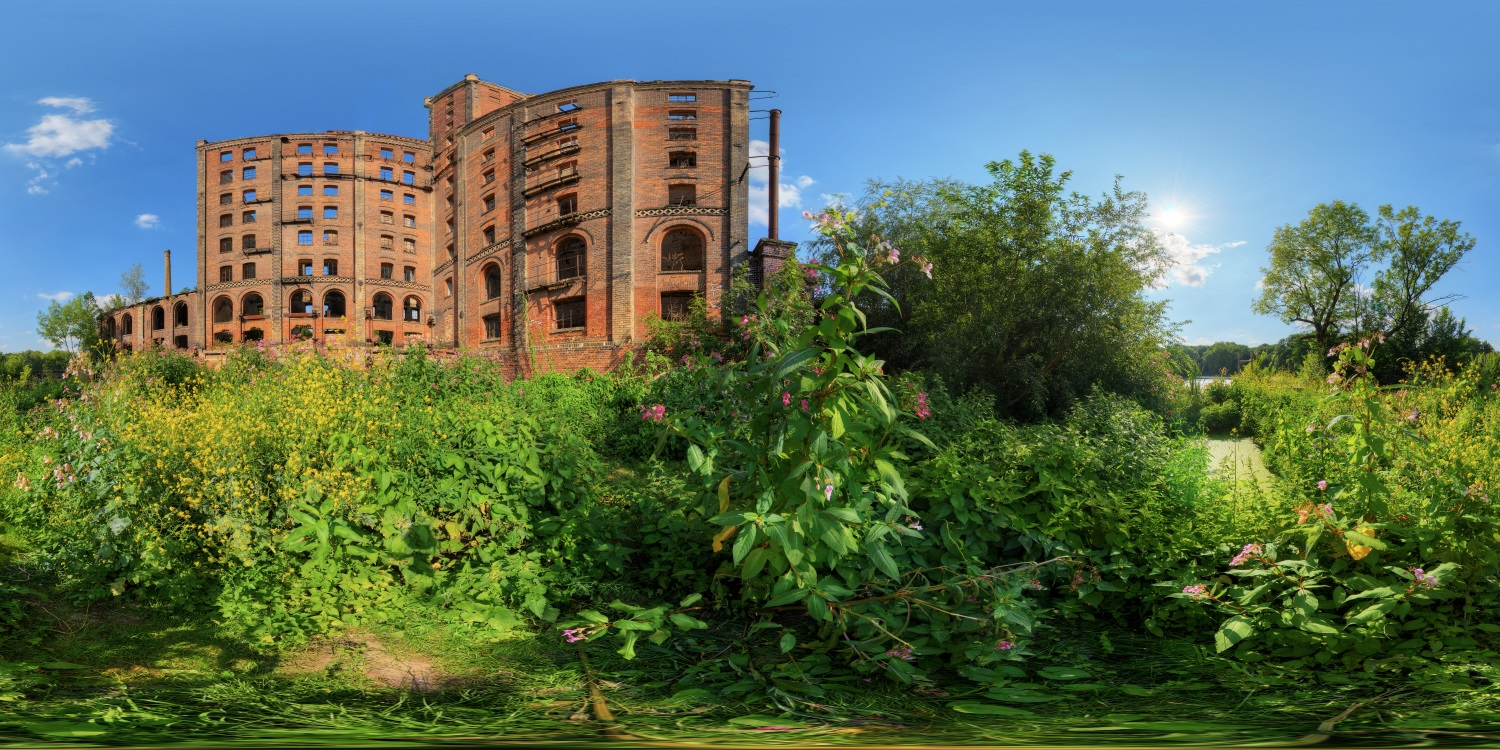
\includegraphics[width=\textwidth]{env_1}}\hfill
    \subfloat{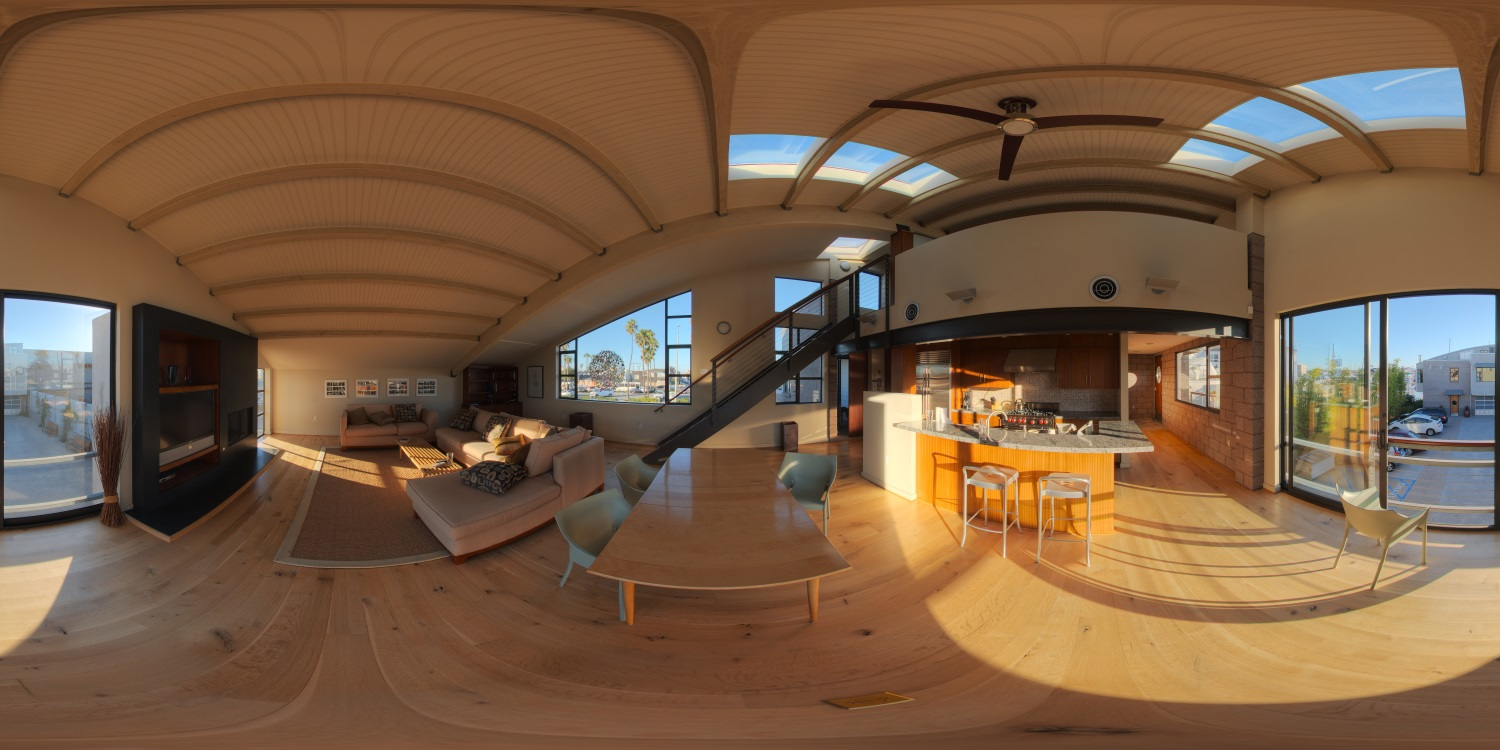
\includegraphics[width=\textwidth]{env_2}}\hfill
    \caption[Environmental textures]{Two examples of environmental textures with equirectangular projections. These were used for backgrounds when rendering and for generating occlusion masks when augmenting.}
    \label{fig:env_1}
\end{figure}

For the realistic backgrounds, we obtained 50 \ac{HDR} environment textures with a resolution of 8000x4000 from \textcite{sibl}. These textures had equirectangular projections, which meant that they could be projected 360 degrees around the head model without distortion. Two samples of environment textures can be seen in figure \ref{fig:env_1}. For non-realistic face textures, 70 different textures, with an average resolution of 1600x1600, were obtained from \textcite{textures}. Most of these textures were of natural materials and some were completely synthetic. Examples of these material textures can be seen in figure \ref{fig:face_textures_1}, along with the realistic face texture and the 1/f noise texture.

\begin{figure}
    \subfloat[Realistic texture]{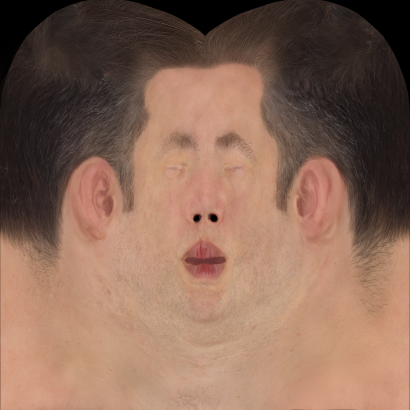
\includegraphics[width=.48\textwidth]{face_texture_1}}\hfill
    \subfloat[1/f noise texture]{
\includegraphics[width=.48\textwidth]{noise_1}}\hfill
    \subfloat[Material texture 1]{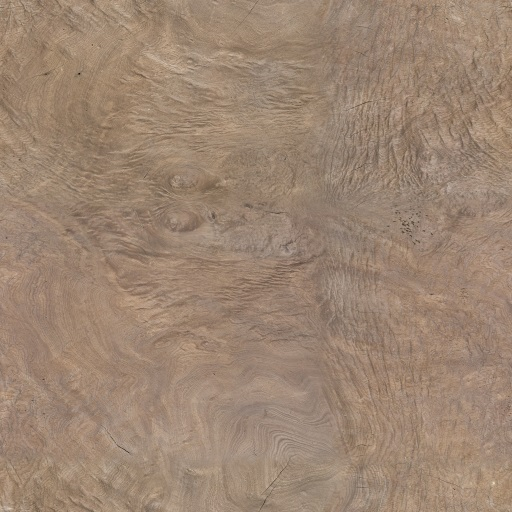
\includegraphics[width=.48\textwidth]{face_material_1}}\hfill
    \subfloat[Material texture 2]{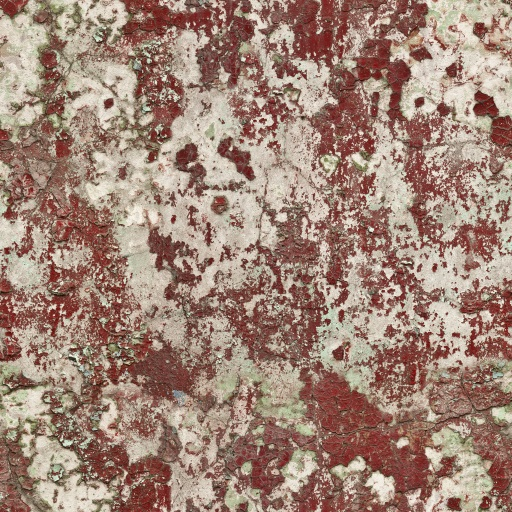
\includegraphics[width=.48\textwidth]{face_material_2}}\hfill
    \subfloat[Material texture 3]{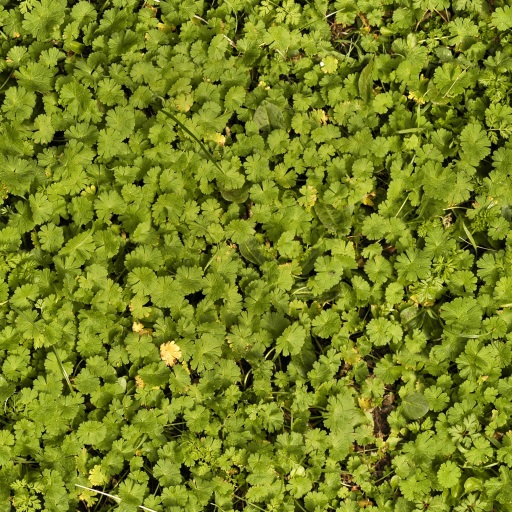
\includegraphics[width=.48\textwidth]{face_material_3}}\hfill
    \subfloat[Material texture 4]{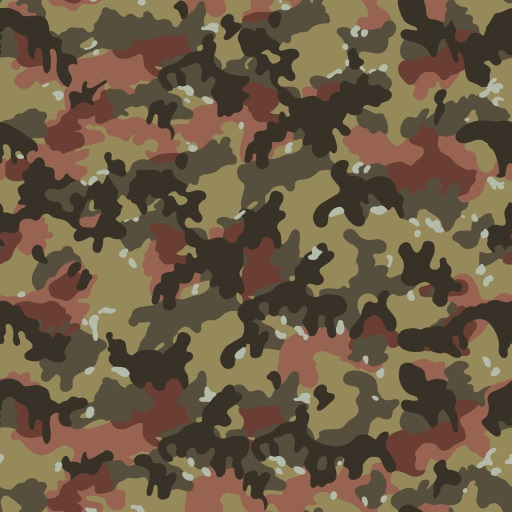
\includegraphics[width=.48\textwidth]{face_material_4}}\hfill
    \caption[Head model textures]{A sample of different textures used for rendering the head model.}
    \label{fig:face_textures_1}
\end{figure}

We started with very simple gray renderings (see figures \ref{fig:head_gray_1} and \ref{fig:head_gray_collage_1}) and then proceeded to more complex materials as it became evident that with the simpler materials it was not possible to successfully train the network. The idea behind using the 1/f noise textures (see figures \ref{fig:head_noise_1} and \ref{fig:head_noise_collage_1}) was that the 1/f noise follows the power spectra of natural images \cite{Schaaf1996}. The results were not that good, and we further experimented with different kinds of materials: completely realistic and completely non-realistic (see figures \ref{fig:head_material_texture_1} and \ref{fig:head_material_texture_collage_1}). In the end, we ended up with a head material that was a mixture of realistic face textures and non-realistic material textures. The material texture was first blended with a random solid color, and this blend was further blended with a realistic face texture. The blending amounts were also randomized. The actual \ac{BRDF} of the head material was a random blend between diffuse and glossy \acp{BRDF}. Samples of images with these blends can be seen in figure \ref{fig:head_final_texture_collage_1}. This figure also has the final amount of randomization in all the rendering parameters. Here is a detailed list of all the randomizations we did per each rendered training sample:

\begin{itemize}
    \item The head model scale was randomized in all three dimensions separately using a uniform random distribution.
    \item The head model rotation was randomized around all three axes separately using a Gaussian random distribution with zero mean. The standard deviations were set so that the 99.9th percentiles of the angles were as follows: pitch angle $\pm\ang{40}$, roll angle $\pm\ang{45}$, and yaw angle $\pm\ang{90}$.
    \item The head model was randomly deformed with Blender's simple deform modifiers of twist, bend, taper, and stretch.
    \item The head model was randomly deformed with Perlin noise \cite{Perlin2002}.
    \item The camera focal length was randomized using a uniform random distribution.
    \item The camera shift in the XY-plane was randomized using a Gaussian random distribution with zero mean. The standard deviation was set so that the 99.9th percentile shift moved the head model at most two-thirds out of the frame.
    \item The direct light direction was randomized using a uniform random distribution. The direction was restricted so that the light never shone behind the head model.
    \item The noise texture scale and translation were randomized using a uniform random distribution. The scaling was identical in all three dimensions.
    \item A random environment texture was selected from a set of 50. Its scale and rotation were randomized using a uniform random distribution. The scaling was identical in all three dimensions, and the rotation was different for each of the three axes.
    \item A random material texture was selected from a set of 70. It was rotated and scaled in the same manner as the environment texture.
    \item A random realistic facial texture was selected from a set of 2. The texture was randomly flipped around the vertical axis.
    \item A random solid color was selected which was blended with the material texture with a random amount. This resulting mix of a solid color and a material texture was then blended with the selected realistic facial texture with a random amount.
    \item The head material \ac{BRDF} mix between diffuse and glossy was randomized. Also, the roughness of the glossy material was randomized.
    \item A random expression was selected from a set of 178 and applied to the head model. Because there were much more expressions with an open mouth, the randomization process was biased so that there would be a 50/50 split between expressions with an open mouth and expressions with a closed mouth.
    \item The Blender Cycles renderer seed value was randomized.
\end{itemize}

\begin{figure}[p]
    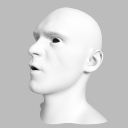
\includegraphics[width=0.3\textwidth]{head_gray_1}\hfill
    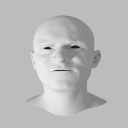
\includegraphics[width=0.3\textwidth]{head_gray_2}\hfill
    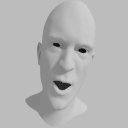
\includegraphics[width=0.3\textwidth]{head_gray_3}
    \caption[Gray head renders]{Head renders with gray background and face textures. A collage of these renders can be seen in figure \ref{fig:head_gray_collage_1}.}
    \label{fig:head_gray_1}
\end{figure}

\begin{figure}[p]
    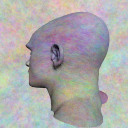
\includegraphics[width=0.3\textwidth]{head_noise_1}\hfill
    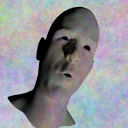
\includegraphics[width=0.3\textwidth]{head_noise_2}\hfill
    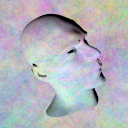
\includegraphics[width=0.3\textwidth]{head_noise_3}
    \caption[Noise head renders]{Head renders with 1/f noise background and face textures. A collage of these renders can be seen in figure \ref{fig:head_noise_collage_1}.}
    \label{fig:head_noise_1}
\end{figure}

\begin{figure}[p]
    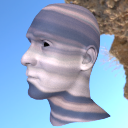
\includegraphics[width=0.3\textwidth]{head_material_texture_1}\hfill
    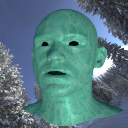
\includegraphics[width=0.3\textwidth]{head_material_texture_2}\hfill
    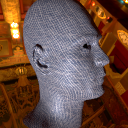
\includegraphics[width=0.3\textwidth]{head_material_texture_3}
    \caption[Non-realistic head renders]{Head renders with realistic background textures and non-realistic face textures. A collage of these renders can be seen in figure \ref{fig:head_material_texture_collage_1}.}
    \label{fig:head_material_texture_1}
\end{figure}

\begin{figure}[p]
    
\includegraphics[width=0.3\textwidth]{dummy1}\hfill
    
\includegraphics[width=0.3\textwidth]{dummy1}\hfill
    
\includegraphics[width=0.3\textwidth]{dummy1}
    \caption*{}
\end{figure}

\begin{figure}
    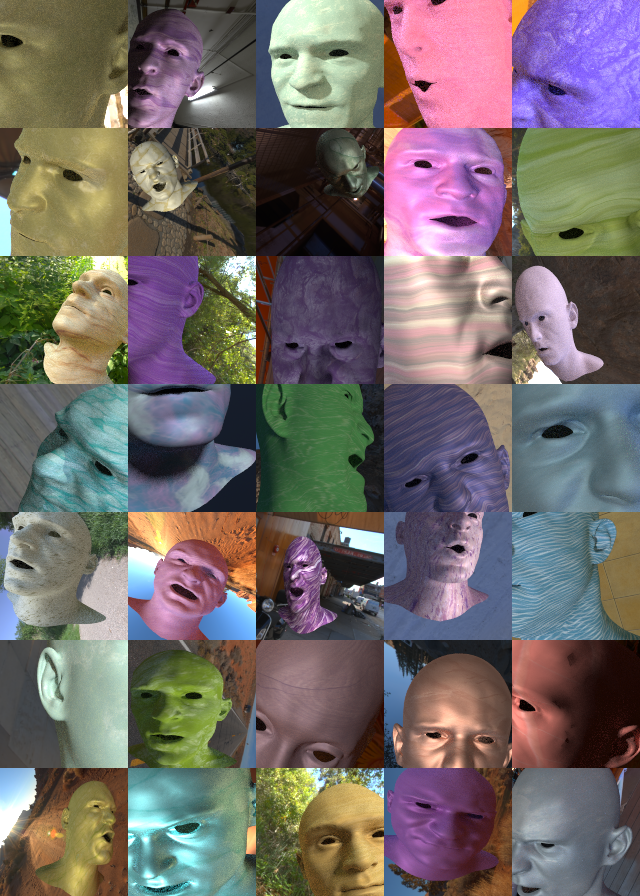
\includegraphics[width=\textwidth]{head_final_texture_collage}
    \caption[Mixed head render collage]{A collage of head renders with realistic background textures and mixed material/realistic face textures. These have the final amount variation between all the randomized rendering parameters.}
    \label{fig:head_final_texture_collage_1}
\end{figure}

\begin{figure}
    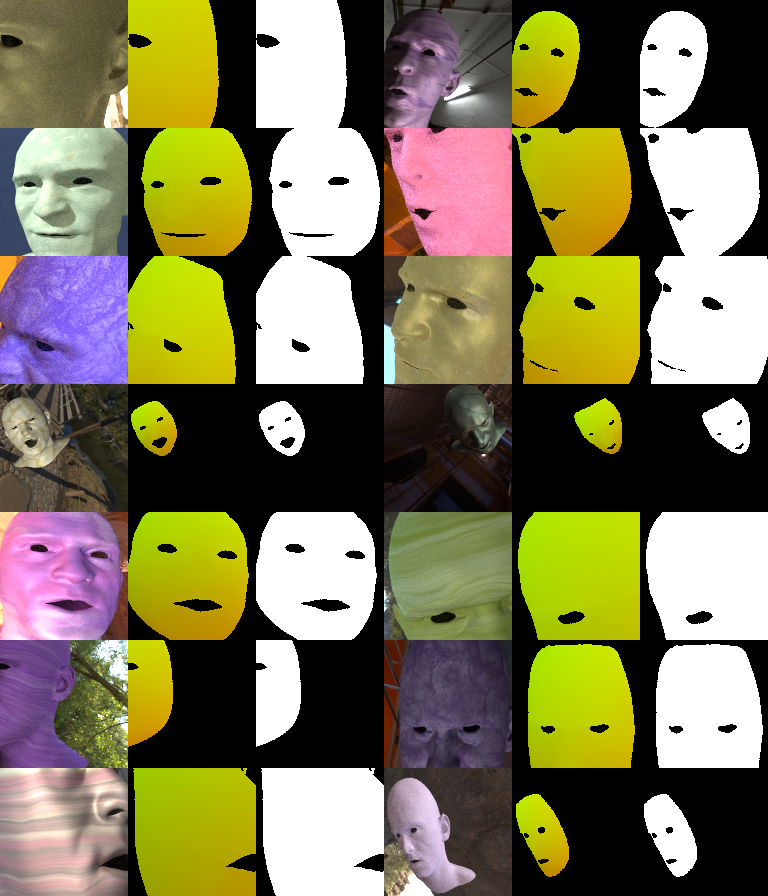
\includegraphics[width=\textwidth]{head_final_triplet_collage}
    \caption[Head triplet render collage]{A collage of head renders with the input, target UV and target mask images. These image triplets formed the training samples.}
    \label{fig:head_final_triplet_collage_1}
\end{figure}

One training sample consisted of three images: the input image, the target UV image, and the target mask image. All the images had a resolution of 128x128 pixels, and they were created from the same randomized rendering parameters. The UV and mask images were rendered with the help of another mask image that segmented out only the frontal face area of the head model. This was done because we were not interested in teaching the network the geometry of the neck or back of the head. Eyes and inside of the mouth with teeth were not included with the original head model, and we did not have assets to model them, so they were left out of the renders. Eyes and inside of the mouth were rendered as black in all three of the training sample images. The resulting image triplets are illustrated in figure \ref{fig:head_final_triplet_collage_1}.

Our rendering loop started by doing all the rendering parameter randomizations. It then rendered the same scene three times, adjusting internal blender settings to generate the different images in the training sample. A random 16 character string was created, and with it, the file names for current rendering sample. Our file naming scheme allowed later the grouping of the rendered files into training samples, whose order could be randomized easily without having to worry about mixing the images.

All the rendering results were stored in floating-point precision. We used the EXR file format with 16-bit floats and ZIP compression. Halving the precision from 32 bits to 16 bits did not affect the results, but reduced the size of the training dataset by a factor of two. The additional built-in ZIP compression reduced file sizes even further, as the UV and mask images were composed of somewhat repeating values. The floating-point precision was essential, especially with the UV images, where the pixel needs to store a real-valued coordinate in the UV space. At first, we used 8-bit precision with the UV images, as is used in the PNG format, and the resulting network did not perform well. In addition, the physically based lighting of the Cycles renderer and \ac{HDR} environment textures generated \ac{HDR} input images. We wanted to save this information so that the data augmentation process would have as much information available as possible.

Antialiasing with 64 samples per pixel was used for input and mask images but disabled for the UV images, where only the center of the pixel was sampled. At the internal facial geometry boundaries, for example between nose tip and upper lip when looked from above, two adjacent pixels could have a considerable distance in the UV space. This is why we reasoned that antialiasing the UV images did not make sense, as it would blur the boundary and generate an invalid UV value. When sampling the pixel centers, it could be possible to find a pixel where the center is inside the model geometry, but part of the pixel is already outside. We did not want to include these pixels in the UV image. We decided to render the mask image with antialiasing which would make these boundary pixels grayscale. These grayscale values could then be thresholded out, and a little bit smaller mask could be created. This mask has pixels that are all 100\% inside the facial geometry and could be used to remove all ambiguous pixels from the UV image.

The rendering speed was about one training sample per second on a modern four-core desktop machine. Most of the time was spent rendering the input image; the UV and mask images were much faster to render in comparison. We kept the sample count per pixel low, at 64, on the input image to keep rendering times in control. Low sample counts caused some noise to be left in the input images, but we reasoned that it does not matter as noise is added anyway in the augmentation process.

Rendering 100 000 training samples would have taken too long on a single machine, so the rendering was offloaded to Aalto Triton and \ac{CSC} Taito computing clusters. The \ac{CPU} utilization of a single Blender rendering process was rather low. It was found out that an optimal combination was to request a job allocation with eight cores and then launch eight separate Blender rendering processes which each was told to use four threads. This way the rendering could reach near 100\% \ac{CPU} utilization, and we witnessed the fastest total rendering times. Each job output the rendered images into the local temporary storage, and after having finished rendering, stored all the images into a tar-archive and sent the file to a shared work directory. After all the jobs had finished, the smaller archives were gathered together and combined into one single large archive. The size of an archive containing 100 000 training samples was around 10 gigabytes.

\section{Neural network design}
\label{sec:net_design}

At the time of starting this project, there were two machine learning Python frameworks that we looked at, \textcite{tensorflow} and \textcite{cntk}. It quickly became clear that the syntax of \ac{CNTK} was simpler, and the examples and tutorials were easier to understand. Back then, Tensorflow did not have an official well-working \ac{GPU} implementation on Windows. In contrast, \ac{CNTK} natively supported \ac{GPU} training without syntax changes on both Windows and Linux. \ac{CNTK} also promised easy-to-use multi-\ac{GPU} training out-of-the-box. The main development of this project was to be done on Windows, and all the training was to be done on Linux servers. So, it was an easy decision to go with the \ac{CNTK} framework.

\begin{figure}
    %\centerline{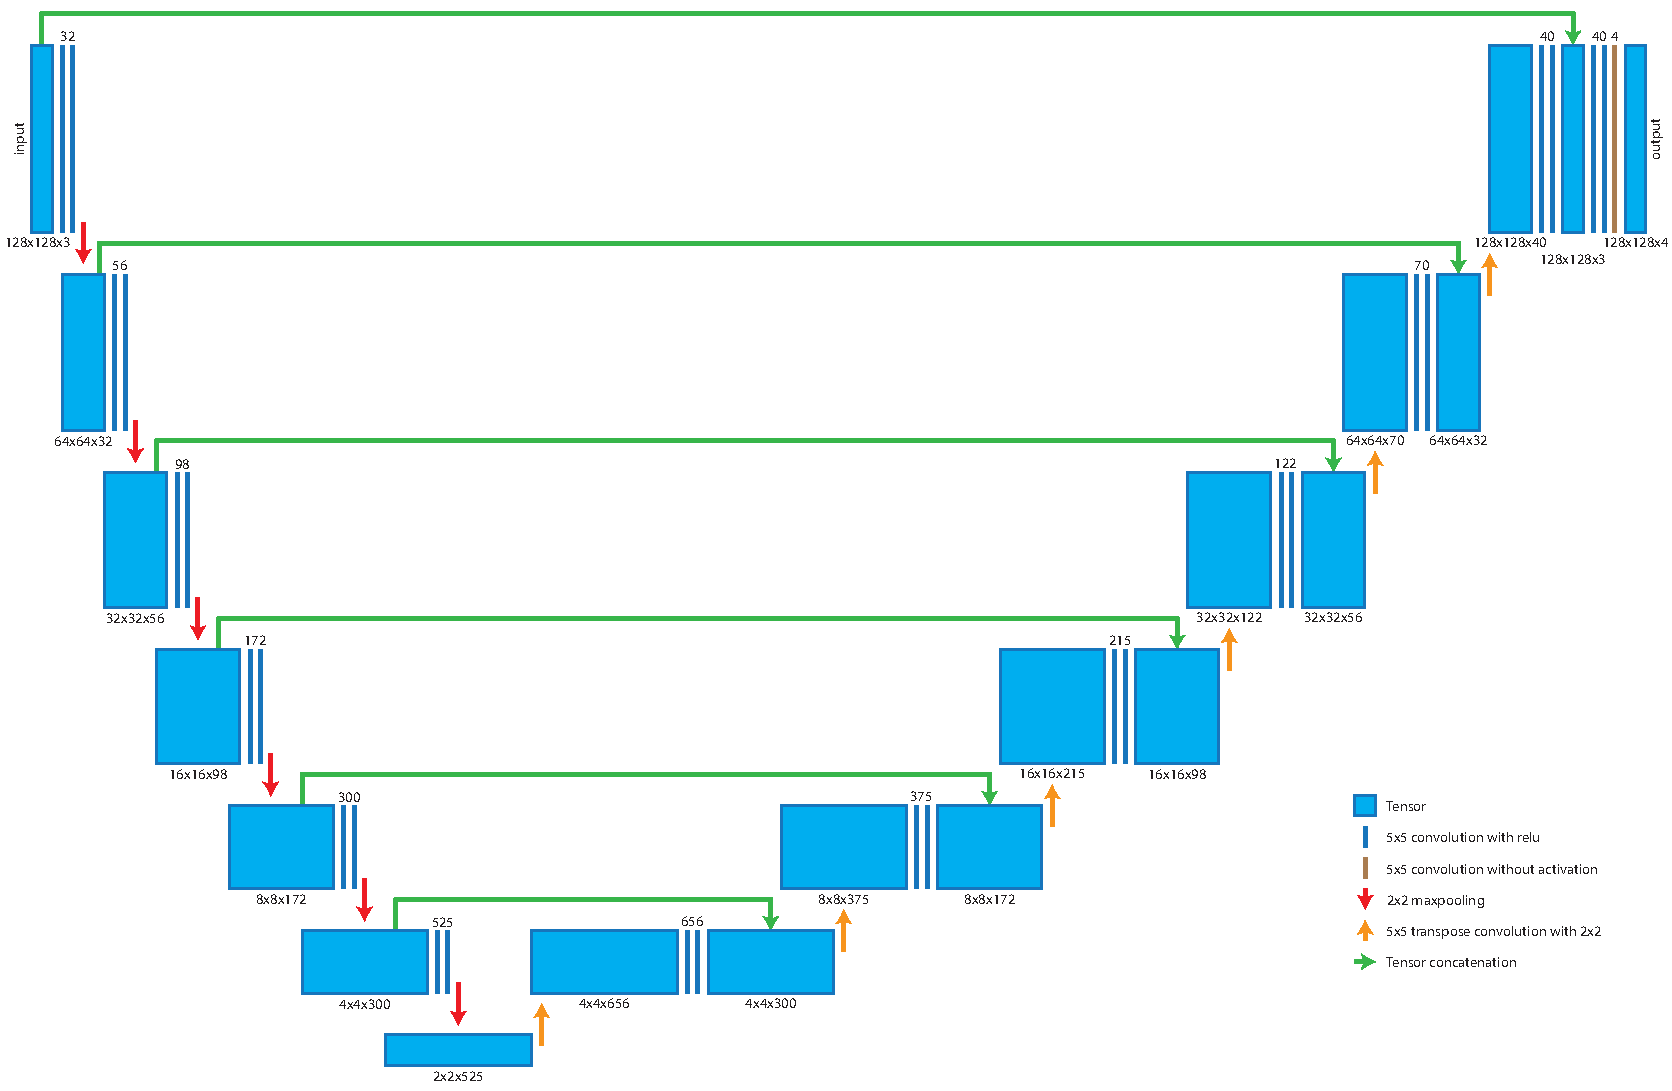
\includegraphics[angle=90,scale=0.85]{uv-net-topology}}
    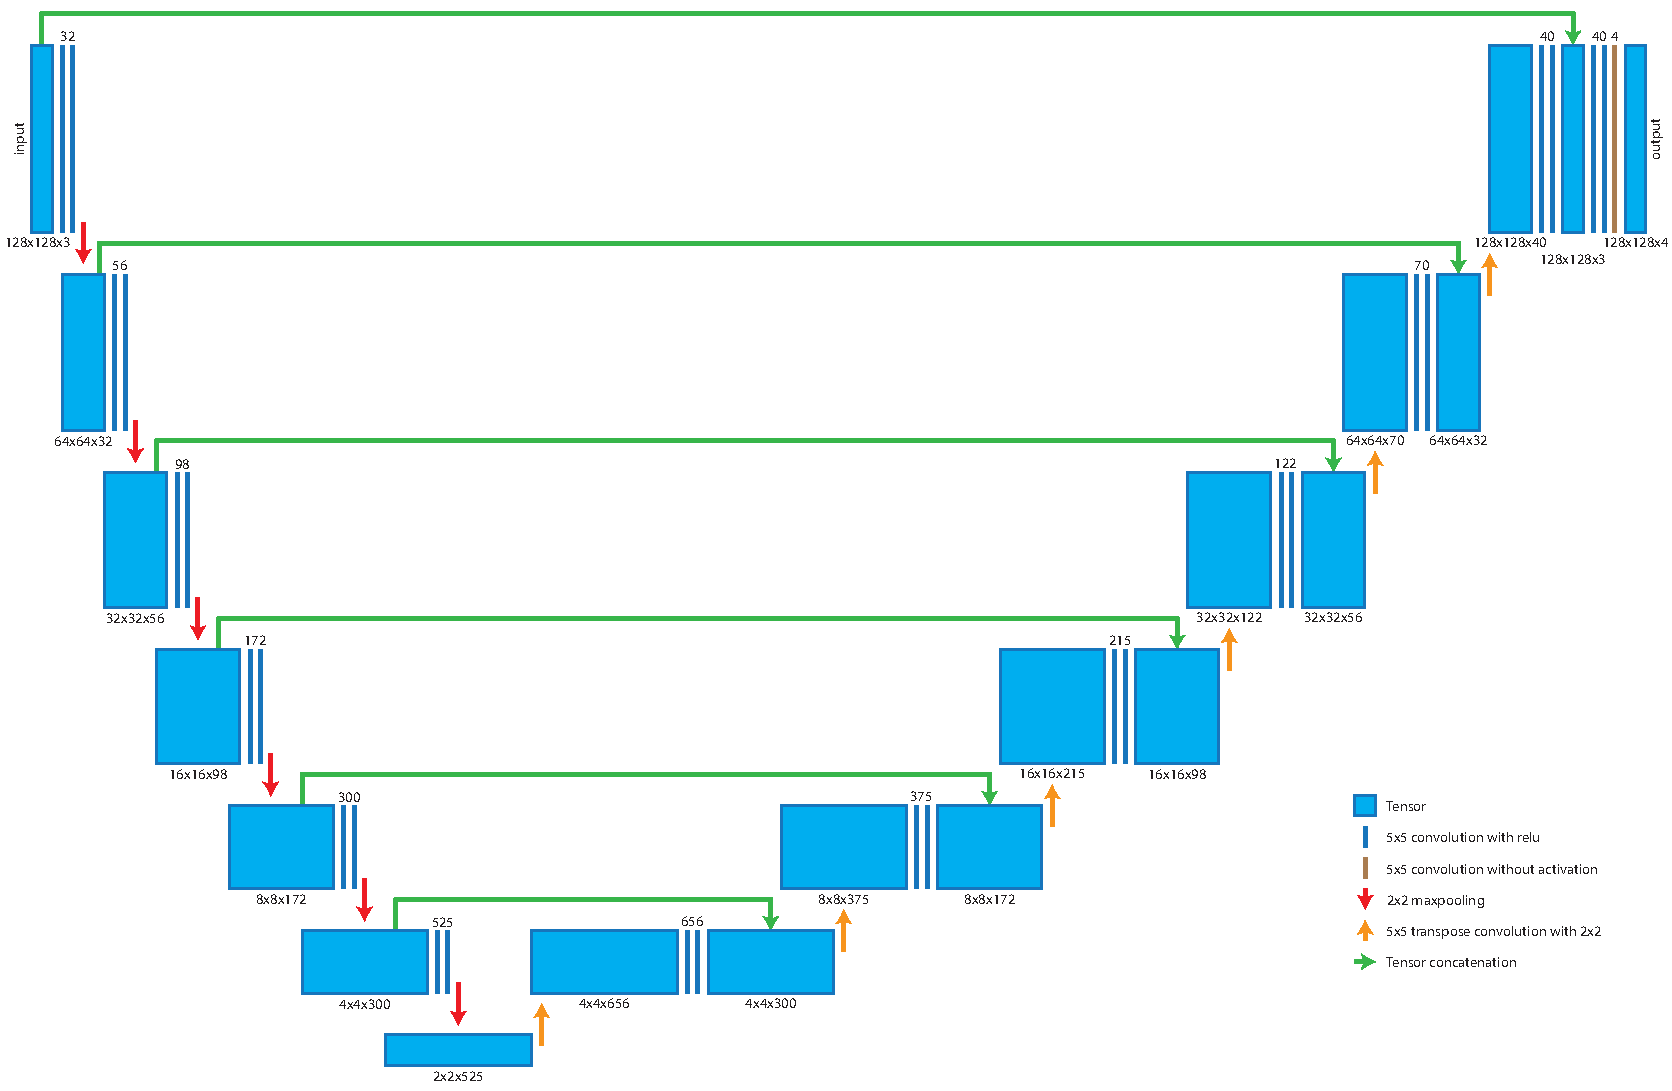
\includegraphics[angle=90,width=\textwidth]{uv-net-topology}
    \caption[Neural network topology]{The final topology of the neural network. It was a fully convolutional network with skip connections between down and upsampling portions. Downsampling was done with max-pooling and upsampling with transpose convolutions. Numbers above the convolution layers convey their feature map sizes.}
    \label{fig:net_top_1}
\end{figure}

Our final network topology is illustrated in figure \ref{fig:net_top_1}. The design relied heavily on the U-net design proposed by \textcite{Ronneberger2015}. The decision to go with the U-net design was influenced by our prior good experiences with it. We decided to call our network UV-net as an homage to its inspirator and because the network did UV mapping. The network was an \ac{FCNN} with skip connections. The input was one image, and the output was three different images of the same size. The skip connections were a vital part of the network, as they were able to preserve the high frequency detail of the input image. Without the skip connections the training process was not able to converge to any satisfactory result.

In figure \ref{fig:net_top_1} the cyan boxes represent the data flowing through the network, the tensors. Tensors are multidimensional arrays of numerical values. In our case, the first tensor was a 128x128x3 floating-point array representing an RGB color image with a resolution of 128x128. The tensor then got processed through the seven levels of the network. At the contracting side of the network, the spatial size of the tensor got reduced but, feature map size increased. In the middle, the tensor size was 2x2x525. At the expanding side, the spatial size was gradually increased, and feature map size decreased. At the end, the network output a tensor with a size of 128x128x4. This included two channels for the UV image and two channels for the two different mask images: normal mask and occluded mask. The skip connections were implemented by first making sure that the spatial dimensions of all tensors on the same level were identical and then just concatenating the tensors together along the feature map axis.

Figure \ref{fig:network_layers_1} illustrates the different layers we used to operate on the tensors. Convolution layers with a filter size of 5x5 were used to extract features from the tensors. For example, the first tensor with three feature maps was convolved with 32 different convolution filters to generate a new tensor with 32 different feature maps. Convolutions used a stride of 1x1, and the input was zero padded to prevent the spatial size reduction of the tensors. The actual downscaling of the tensors was done with 2x2 max-pooling layers \cite{Goodfellow2016}. Each feature map was scanned through looking at disjoint 2x2 pixel areas at a time. Whatever pixel had the highest value was selected. This reduced the spatial dimensions of the tensors by a factor of two. Max-pooling layers also introduced some invariance towards the internal shifting of features. Upscaling of the tensors was done with transpose convolution layers with a filter size of 5x5. These effectively did the same as the convolution layers but in reverse. If a stride larger than one was used, 2x2 in our case, the spatial dimensions of the tensors were increased. The output size would not be the same as if scaled up by a factor of two. This was remedied by just cropping the tensors back to the right size.

\begin{figure}
    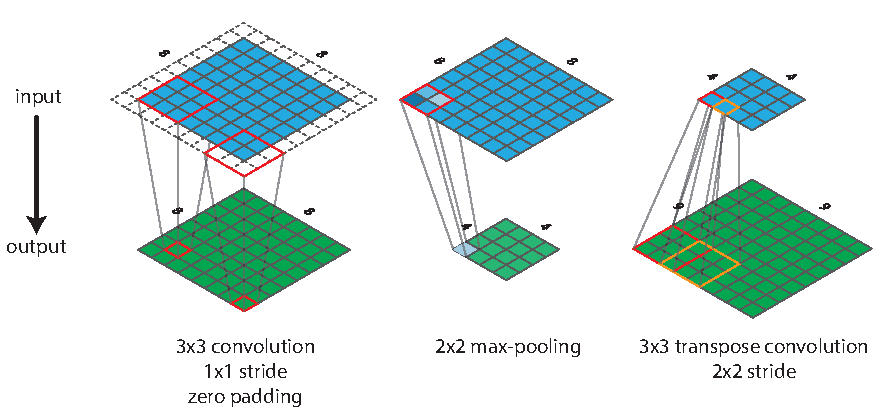
\includegraphics[width=\textwidth]{network-layers}
    \caption[Network layers]{A visualization of the different layers used in the network. Zero padding was used with the normal convolution layers to keep the output same size. Max-pooling layers selected the maximum value inside a 2x2 area, effectively reducing the size by a factor of two. Transpose convolutions with a stride of two were used to upscale. 3x3 convolution filter size is used here for illustration purposes; the final filter size was 5x5.}
    \label{fig:network_layers_1}
\end{figure}

We used exponentially growing feature map sizes as fully convolutional neural networks like ours need large feature map sizes to work well \cite{Ronneberger2015}. We started with 32 initial feature map size and increased that by a factor of 1.75 for every level. On the upscaling side of the network, the feature map sizes were derived from those on the downscaling side by multiplying by 1.25. This was because the network needed more expressivity on the upscaling part for generating dense pixel mappings.

We preferred using two convolution layers in succession with smaller filter sizes to using one convolution layer with a larger filter size. This increased the effective receptive field size of the convolutions while not increasing needed parameter count as much. For example, with two 5x5 filters, the effective receptive field size was 9x9. Two 5x5 filters needed 50 trainable parameters, and one 9x9 filter would have needed 81 trainable parameters.

The convolution layer filter values were prepared using uniform Glorot initialization, described by \textcite{Glorot2010}. All the layers had the bias term enabled. After testing all the available activation functions, we decided to use the \ac{RELU} \cite{Goodfellow2016}. It was fastest to train and gave as good results as the more recent ones, like the \ac{ELU} \cite{Clevert2015}. The last convolutional layer did not have any activation function.

Every part of the network model creation was parameterized. The full network creation code can be seen in listing \ref{appendix:network_code}. This parametrization allowed easy changing of the network topology. Parameters could also be saved to a file and read back later. This made it simple to generate hyperparameter sweep runs on the computing clusters.

\section{Loss function design}
\label{sec:loss_func}

A fully convolutional neural network like ours can be trained in a supervised manner using input/output image pairs. We had hundreds of thousands of these image pairs thanks to the synthetic training data generation process. The network was first given in an input image, and then the generated output images were compared with known ground truth images. The difference between these images could then be used to iteratively update the network parameters to gradually make the output more and more like the ground truth images.

A general overview of the image data flow during processing one training sample and calculating its loss is illustrated in figure \ref{fig:train_sample_1}. The process was started by reading in the current training sample which consisted of input, target UV, and target mask images. The target mask image was thresholded so that the grayscale pixels were turned to black. The target UV image was multiplied with this new slightly smaller target mask image. This removed all the ambiguous border pixels from both the target UV and target mask images.

The original input image and the thresholded target UV and target mask images were then input into the data augmentation process. The process output an augmented input, target UV, and target mask images. In addition, it generated two new mask images: an occluded target mask image and an eroded target mask image. The occlusions in the occluded target mask image reflected the colored occlusions generated onto the augmented input image. The eroded target mask image had a morphological erosion image processing operation applied which increases the size of the black areas and decreases the size of the white areas.

The augmented input image was given to the neural network which generated three output images: result UV, result mask, and occluded result mask. The UV image generated was not masked straight out of the network, so it was multiplied by the augmented target mask to create the final masked result UV image. Result mask and occluded result mask images were left as is.

\begin{figure}
    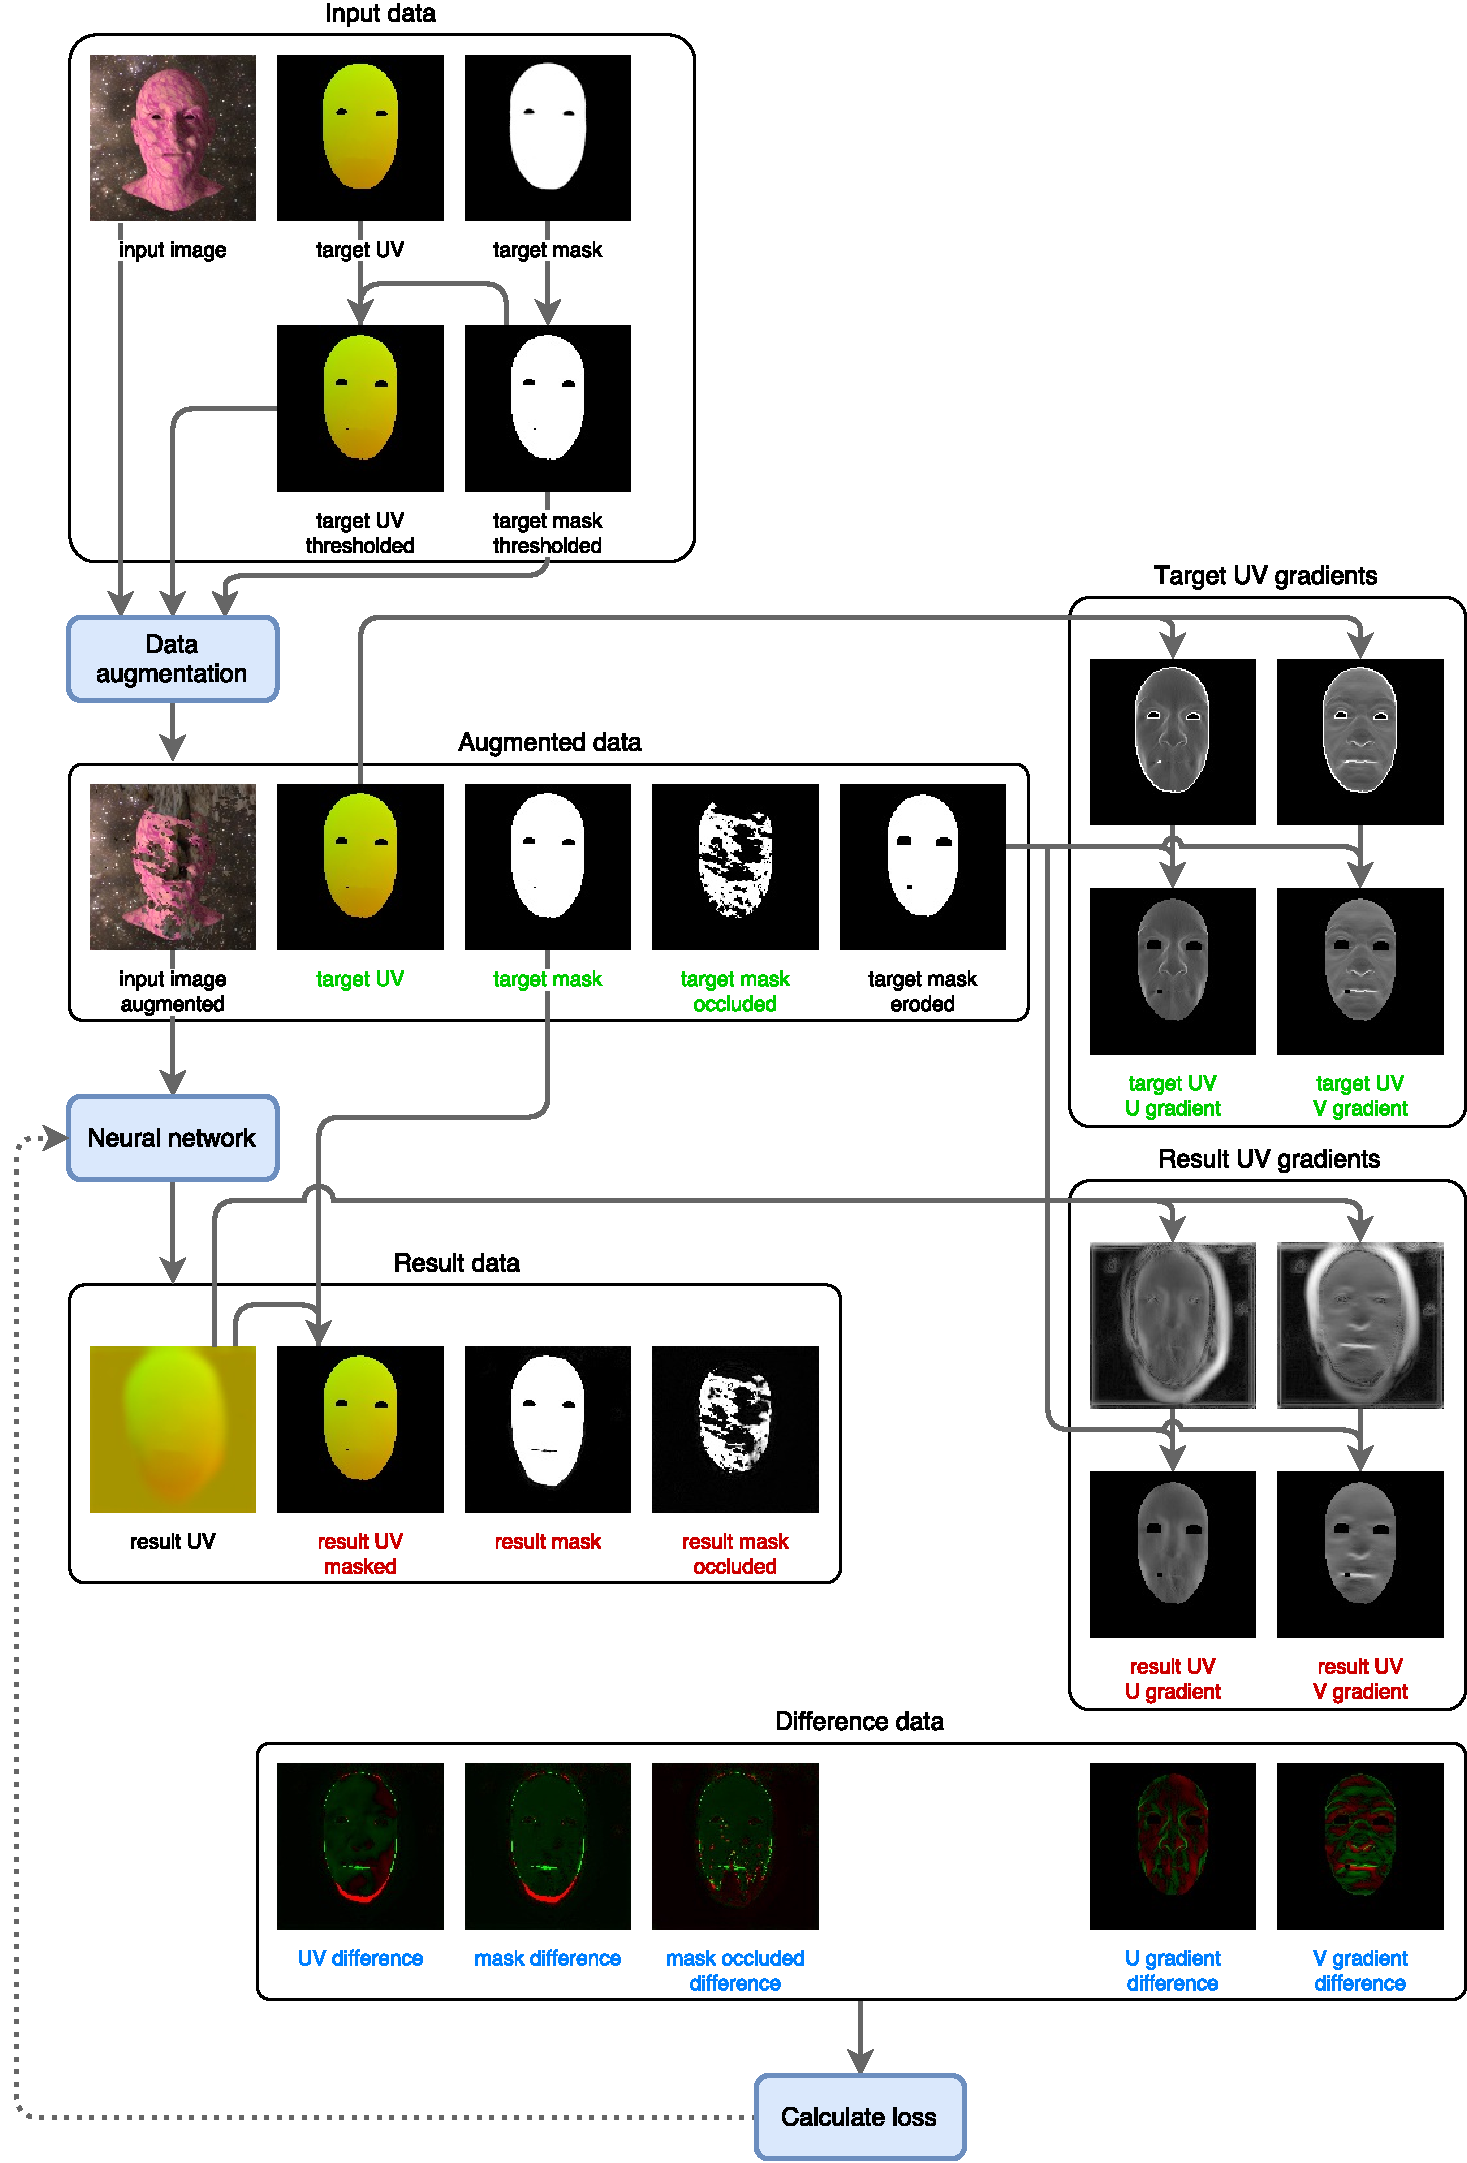
\includegraphics[width=\textwidth]{train-sample}
    \caption[Training sample]{An overview of the data flow when evaluating one training sample. The input data is first preprocessed and then fed to the data augmentation process. From the augmented data, the augmented input image is given to the neural network. The network will output result data which is slightly post-processed. The difference data calculation has not been visualized using arrows but with colors. The result images with red labels are subtracted from the target images with green labels to produce the difference images with blue labels. The actual final loss value is calculated from the difference images with the method illustrated in figure \ref{fig:loss_function_1}. The images on the right side of the figure on this page are the UV gradient images. Gradient images tell how much pixel values change when moving from one pixel to the next. The eroded target mask is used to eliminate large gradient values that exist on, for example, the outer edges of the face.}
    \label{fig:train_sample_1}
\end{figure}

\begin{figure}
    \centerline{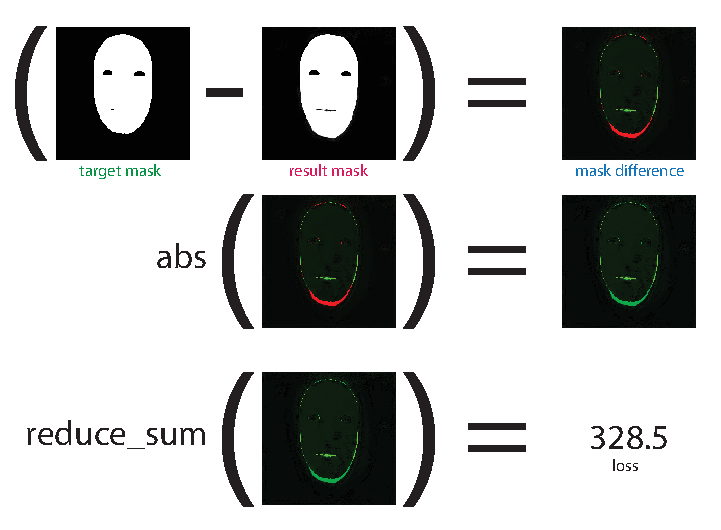
\includegraphics[width=0.75\textwidth]{loss-function}}
    \caption[Loss function]{A visualization of the L1 loss function evaluation for the images. The difference between the images was calculated by a pixel-wise subtraction. Positive values are depicted in green color and negative in red color. The absolute operator turned all pixel values to positive, and the reduce-sum operator summed up all the pixels together to one scalar value.}
    \label{fig:loss_function_1}
\end{figure}

A gradient image describes how much pixel values change between adjacent pixels. We knew that the UV image should mostly have very smooth changes within itself, i.e., no bumpiness or splotchiness in the gradient images. This is because the UV color mapping process inherently generates smoothly varying colors from the smooth UV space. Occasional sharp jumps might be generated by, for example, the nose geometry. Because the UV image should be smooth, its gradient image should, therefore, contain only small gradient values and the sum of the pixels in the gradient image should be low. Thus, low gradient image pixel sum could be used as an additional loss term to help steer the training process towards smoother result UV images.

Gradient images were calculated from both the augmented target UV image and the non-masked result UV image. Gradients were calculated in both X and Y directions for both of the U and V channels, which generated four new images. Figure \ref{fig:train_sample_1} depicts the gradients as vector magnitudes for U and V channels using only one image per each. A problem with the gradients was large values at the edges of the face, mouth and eyes. We were not interested in these as they did not introduce any new actionable information to the process. We remedied the problem by multiplying the gradient images with the previously generated eroded target mask image. This had the desired effect of removing the large edge gradient values from the gradient images.

Figure \ref{fig:train_sample_1} labels the images, between which the loss was calculated, with green and red. The final loss value calculation method is shown in figure \ref{fig:loss_function_1}. The difference between two images was calculated by doing a pixel-by-pixel subtraction. In the difference image, green values depict positive values and red negative values. The absolute operation was then applied to the image resulting in positive values only. All the pixel values were summed over the image resulting in one scalar value. A total of seven of these scalar values were produced, and they were summed together to form the final loss value. To summarize, our loss function was an L1 loss of the UV, UV gradient, mask, and occluded mask images. We tried different combinations of L1 and L2 losses and, in the end, the L1 loss always outperformed the L2 loss when it came to the sharpness of the resulting images. The L2 loss tended to produce blurred mask edges and blotches inside the UV mapping. Full code implementation of the loss function can be seen in listing \ref{appendix:loss_code}.

To optimize the loss, we used the Adam optimization method \cite{Kingma2015} provided with \ac{CNTK}. We started with a learning rate of 0.0001 and a momentum of 0.9. After the loss improvements had tapered off, the learning rate was reduced to 0.00001 and momentum increased to 0.99. Also, the magnitude of the noise augmentation was gradually decreased down to zero during the training process.

\section{Data augmentation process}
\label{sec:data_aug}

\begin{figure}
    \subfloat[none]{\label{fig:augmentations_1a}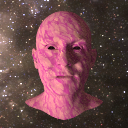
\includegraphics[width=.25\textwidth]{head_augment_none}}\hfill
    \subfloat[rotate]{\label{fig:augmentations_1b}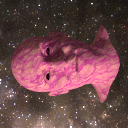
\includegraphics[width=.25\textwidth]{head_augment_rotate}}\hfill
    \subfloat[shuffle]{\label{fig:augmentations_1c}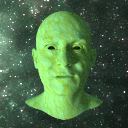
\includegraphics[width=.25\textwidth]{head_augment_shuffle}}\hfill
    
    \subfloat[exposure and \newline gamma]{\label{fig:augmentations_1d}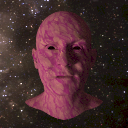
\includegraphics[width=.25\textwidth]{head_augment_expgamma}}\hfill
    \subfloat[noise]{\label{fig:augmentations_1e}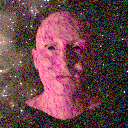
\includegraphics[width=.25\textwidth]{head_augment_noise}}\hfill
    \subfloat[occlusion]{\label{fig:augmentations_1f}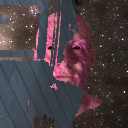
\includegraphics[width=.25\textwidth]{head_augment_occlusion}}\hfill
    
    \centering
    \subfloat[all]{\label{fig:augmentations_1g}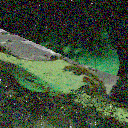
\includegraphics[width=.25\textwidth]{head_augment_all}}
    \caption[Input image augmentations]{Examples of different types of input image augmentations. The final image \protect\subref{fig:augmentations_1g} is the same as \protect\subref{fig:augmentations_1a}, but with all augmentations at their extreme.}
    \label{fig:augmentations_1}
\end{figure}

Without data augmentation, the network did overfit quite quickly. That is, the network learned the training dataset well, but would not generalize to test or real-world images. Data augmentation expanded the existing training dataset many times over. We were able to train a network continuously for ten days without overfitting by combining all our augmentation methods shown in figure \ref{fig:augmentations_1}: rotate, shuffle, exposure, gamma, noise, and occlusions. If the input image in figure \ref{fig:augmentations_1} is compared to the final image with all the augmentations enabled, it is evident that the modifications to the original image could be drastic.

Rotation augmentation (see figure \ref{fig:augmentations_1b}) randomly picked a rotation of 0, 90, 180, or 270 degrees. The input, UV, and mask images were rotated. It should be noted that flip augmentations could not be used in our method, as, for example, flipping along the vertical axis would have made the UV mapping ambiguous. This was not a problem with rotations. The shuffle augmentation (see figures \ref{fig:augmentations_1c} and \ref{fig:head_augment_shuffle_collage_1}) separated the RGB color channels of the input image, shuffled them randomly, and then combined them back into a new image. This effectively increased the training dataset size by a factor of six. The shuffling was done on per color channel, not per pixel. The exposure augmentation multiplied the input image with a random number. The gamma augmentation raised the input image to a random power. These two were used to increase the brightness variation of the input image (see figures \ref{fig:augmentations_1d} and \ref{fig:head_augment_expgamma_collage_1}). The noise augmentation (see figures \ref{fig:augmentations_1e} and \ref{fig:head_augment_noise_collage_1}) added Gaussian noise with random magnitudes to the input image. This was one of the most important augmentations as it made the model much less prone to overfitting. Adding noise made the model generalize better, be less sensitive to small variations in input, and aided the training process to avoid local minima.

\begin{figure}
    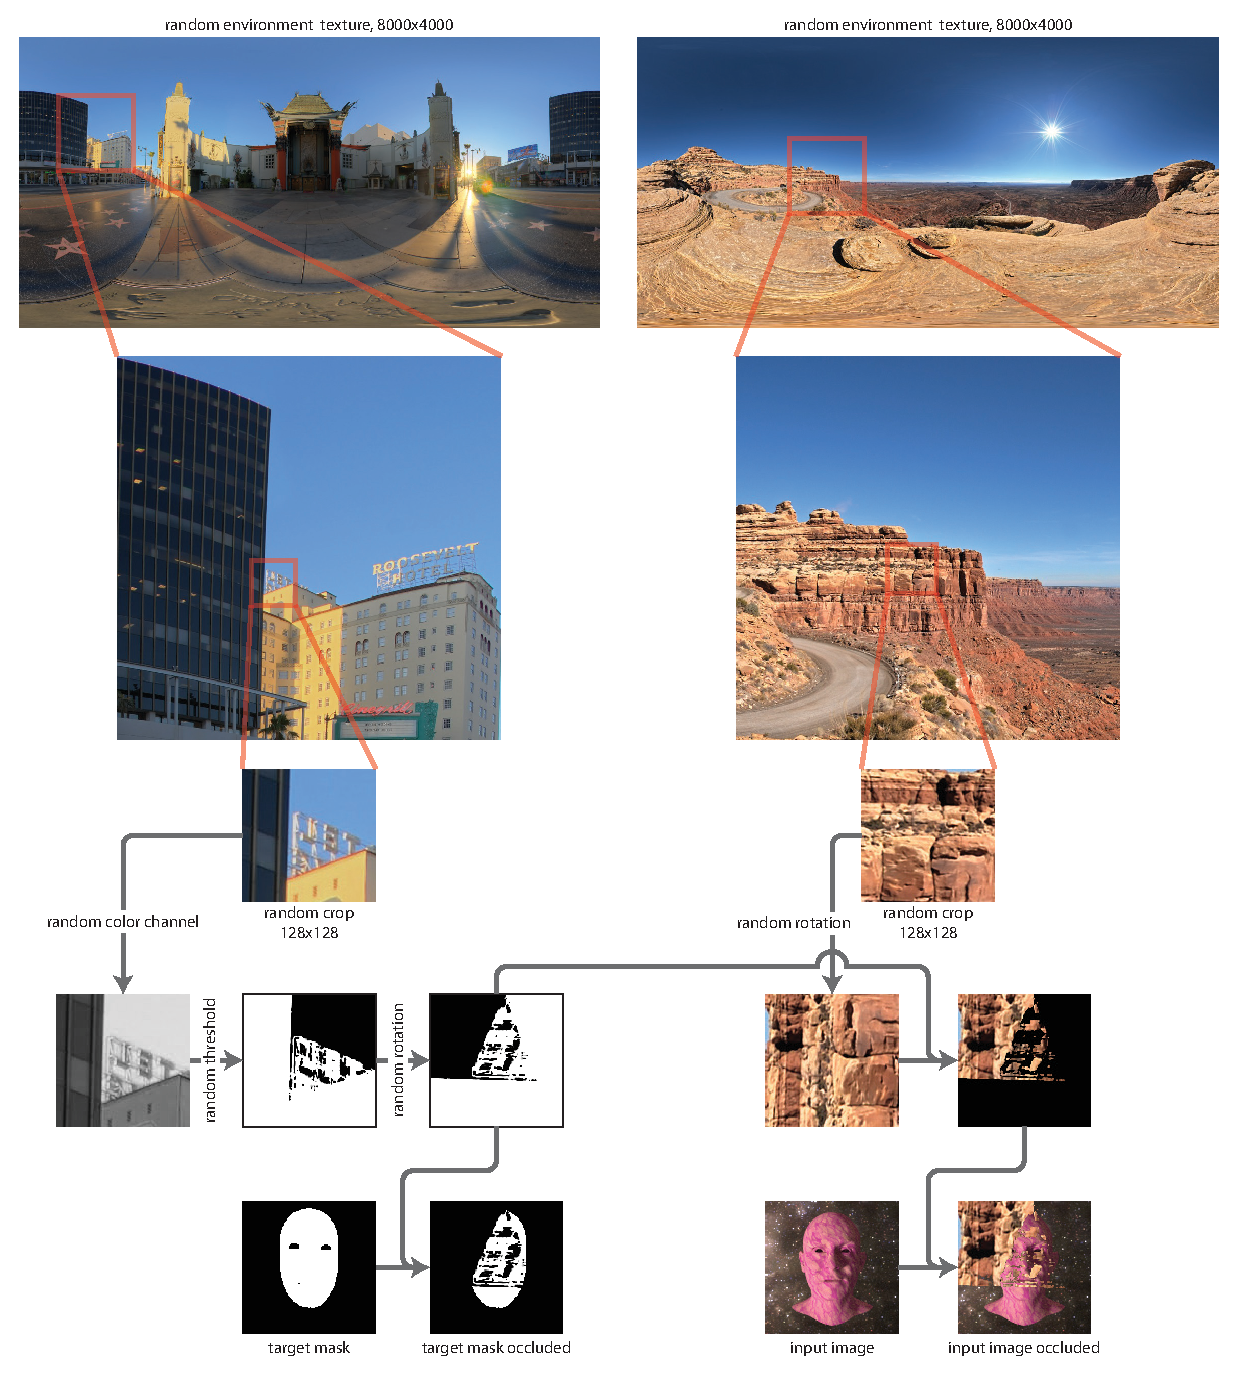
\includegraphics[width=\textwidth]{occlusion-gen}
    \caption[Occlusion generation]{An overview of the occlusion generation process. Two environment textures were selected at random, and a small random area was selected from each of them. These two small images were then used to create the occlusion mask and a color for it.}
    \label{fig:occlusion_gen_1}
\end{figure}

As we evaluated the results, we noticed that any occlusion in front of the face usually degraded the mapping results considerably, usually completely breaking the tracking. Occlusions were, for example, long hair, beards, mustaches, sunglasses, hats and random objects. We did not have assets to add these to the training data, and it would have been infeasible to try to model every kind of possible occlusion. The only way to try to fix this was to add occlusions to the training data, on-the-fly, using augmentation.

Adding rectangular occlusions to the training data, filled with either solid colors or noise, did not improve results. These tended to bias the network to detect every occlusion as a rectangular one. Instead, we decided to use a method that would generate more natural-looking occlusions. The general overview of our method is shown in figure \ref{fig:occlusion_gen_1} and examples of results in \ref{fig:head_augment_occlusion_collage_1}. We obtained 50 \ac{HDR} environment textures from \textcite{sibl}. The textures were of very high resolution, 8000x4000 being the most common one. First, we selected two random pictures from the set. Then, we independently selected a random 128x128 crop from each. The first crop would be used to generate the occlusion mask and the second one would be used to apply color to the mask. This two-step approach was used to increase the randomness of the process, as the mask and its resulting color were not linked together.

\begin{figure}
    \includegraphics[width=\textwidth]{head_final_texture_augmented_collage}
    \caption[All augmentations collage]{A collage of head renders with all the augmentations applied. Images like these were ultimately fed to the network in the training process. Figure \ref{fig:head_final_texture_collage_1} is the same collage without any augmentations.}
    \label{fig:head_final_texture_augmented_collage_1}
\end{figure}

\begin{figure}
    \includegraphics[width=\textwidth]{head_final_triplet_augmented_collage}
    \caption[All augmentations triplet collage]{A collage of augmented head renders with the input, target UV, target mask, and occluded target mask images. The augmentation process mainly touched the input image and generated the occluded target mask. Figure \ref{fig:head_final_triplet_collage_1} is the same collage without any augmentations.}
    \label{fig:head_final_triplet_augmented_collage_1}
\end{figure}

To generate the occlusion mask, a random color channel was selected from the first cropped image and then thresholded. Our thresholding method did not generate binary images, but grayscale images with gradients. This enabled the creation of transparent occlusion masks on top of the input image. The process of creating the threshold image was repeated until the ratio of black to white pixels was within some predetermined range. This range was established by visually inspecting collages of thresholded images and adjusting the target range until there were about equal amounts of black and white. An example of this kind of collage can be seen in figure \ref{fig:occlusion_mask_collage_1}. After successful thresholding, the image was randomly rotated and then multiplied with the target mask to generate the occluded target mask. The random crop from the other texture was also randomly rotated and multiplied with the thresholded image. The resulting color image was then blended over the original input image to create the final occluded input image.

Our rendered data was in floating-point precision, the previously mentioned augmentations were not restricted in range, and our occlusions were based on \ac{HDR} textures. This all meant that our final augmented input image could have values outside the 0.0--1.0 floating-point range. The real-world images that we used for evaluation were in the JPEG or PNG formats. They had 8-bit color channel precision, that is, discrete values between 0 and 255. If a color value like this was converted to floating-point by dividing by 255.0, the result was a value between 0.0 and 1.0 with 255 steps. As a result, for the two final augmentations, we used clipping and quantization. Clipping restricted the color value range between 0.0 and 1.0, and quantization compressed values between this range to 255 distinct values.

A collage of input images with all augmentations applied can be seen in figure \ref{fig:head_final_texture_augmented_collage_1}. Figure \ref{fig:head_final_texture_collage_1} is the same collage without any augmentations. The augmented collage shows that the final training material could be exceedingly non-realistic and hard even for a human to understand. The occlusion method was able to generate a diverse set of colored masks, and sometimes the method even covered the whole face in the image. Figure \ref{fig:head_final_triplet_augmented_collage_1} shows how the whole augmentation process modified the training sample images in general. It can be compared with figure \ref{fig:head_final_triplet_collage_1}. Most of the augmentation methods only touched the input image, the exception being rotation which rotated all images. Occlusion augmentation did not touch the target mask but created a new one, the occluded target mask. This enabled the neural network to detect occlusions while still generating a full, non-occluded, mask image.

\section{Training process}
\label{sec:training_process}

\begin{figure}
    \includegraphics[width=\textwidth]{train-processes}
    \caption[Training software processes]{An illustration of the software processes used during the training and the data flow between them. Red arrows mean starting of a new process.}
    \label{fig:train_processes_1}
\end{figure}

The training process was started by first thinking on a high level what modifications we wanted to do to the network model, loss function, and data augmentation. Because the computing clusters we used had a limit of 20 simultaneous \ac{GPU} jobs, at most 20 different combinations were created. Usually, only a single parameter was changed. Each combination was separately committed to a Git version control repository and tagged with a logical and unique tag name. Then separate jobs, with the tag name as a parameter, were sent to the computing cluster. The first thing the job did was to create a clean working environment and clone the network code from the Git repository with the given tag name. It would also copy and decompress the 100 000 training samples to a local job-specific temporary directory. The job generated a unique run-ID using the tag name and current time. This ID was used to create an output directory to which all the results of the current job would be saved. Doing it this way made it absolutely sure that the network was actually trained with the parameters and training data that it was supposed to. Also, when looking at the results, we could be sure that result files in a specific directory belonged to a specific training run.

After the initial setup was completed, the job launched our Python-based training script. A general overview of the software processes launched at this moment is given in figure \ref{fig:train_processes_1}. The script first listed all files and their paths in the training dataset, grouping them into training sample triplets. \ac{CNTK} was initialized, and it compiled the static graph of the network and readied the target \ac{GPU} for training. The main training loop started to run after that.

All of the data augmentation was implemented in pure Python code, and that proved to be a performance bottleneck. One minibatch contained 40 samples of data and augmenting it took on average the same time as training it. This meant that the \ac{GPU} utilization could only reach 50\% at best. The problem was solved by moving the data augmentation to a separate process using the Python multi-processing module. By doing this, we were able to read and augment the data asynchronously with the training and increase the \ac{GPU} utilization to almost 100\%.

The data reading and augmentation process started by caching the most used files into memory, for example, the environment textures which were used to generate occlusions. The list that contained all the training sample paths was randomized, and the data reading and augmenting loop was entered. The loop started by reading in one minibatch worth of training samples and then augmenting them.  The ready minibatch of data was sent to the main training process by using pipes in the Python multi-processing module. This loop was continued until the end of the training sample path list was reached, or a predetermined number of training samples had been processed. At this point, an epoch was signaled as done. The data reading and augmenting process returned to the sample path list randomization and started the loop again.

Meanwhile, the main training process was reading the minibatches of data from the pipe and sending them to the \ac{GPU} to be processed. This was continued until the epoch done signal was received from the data read and augment process. At this point, the model was evaluated with different evaluation images. The result images were sent to a new plotting process, again, because of Python performance reasons. Plotting all the result images, even after optimizations, took upwards of 30 seconds. The plotting process also updated the result \ac{HTML} file. Next, the main training process returned to the training loop if not enough epochs had been done or the maximum training time limit had not yet been reached. If the limits had been reached, the main process saved the current model parameters to a file and exited.

\section{Visualization methods}
\label{sec:viz_methods}

The generation of the UV mapping allowed us to create various visualizations. They were used to assess the accuracy and stability of the mapping. Accuracy meant how close the generated geometric features matched the actual real geometry and stability how well the features stayed in place while applying the network to video. Any visualization that could be created in the 2D UV space could be easily transferred onto the face. We created four different visualizations: texture projection, inverse texture projection, grid line projection, and grid points projection. Face swapping between two different people and 3D mesh generation should be possible using the mappings, but we did not implement them.

\subsection{Texture projection}

\begin{figure}
    \includegraphics[width=\textwidth]{projection-tex}
    \caption[Texture projection]{Texture projection on the input image. The mapping generated by the network was used to sample a texture, and the result was applied back to the input image.}
    \label{fig:projection_tex_1}
\end{figure}

Texture mapping, using the original texture that came with the model that was used to generate the training data, was an obvious choice for the first visualization. This projection could be used to assess the accuracy of the generated geometry and how similar the looks between the real human and the textured face were. An overview of the texture projection process is given in figure \ref{fig:projection_tex_1}. This method could not take lighting into account, and that is why the textured faces looked flat.

First, a UV map image was created from the input image using the neural network. The UV image was upscaled by a factor of two, and all of its non-black pixels were looped through. Using the UV coordinates encoded to the red and green channels of the pixel, a texture look-up was made. The pixel color value that was read from the texture was written to a new image into the same position as the original pixel in the UV image. The input image was then also upscaled, and the projected image was applied on top of it. Finally, the composite image was downscaled by a factor of two. The images were scaled up and down to introduce a simple antialiasing effect. Without the scaling, the results looked rough and shimmered when applied to a video.

\subsection{Inverse texture projection}

\begin{figure}
    \includegraphics[width=\textwidth]{projection-inv}
    \caption[Inverse texture projection]{Inverse texture projection. The mapping generated by the network was used to transform the input image into the UV domain using bilinear filtering. Result image can be compared to the reference texture.}
    \label{fig:projection_inv_1}
\end{figure}

As the name suggests, the inverse texture projection did the same thing as texture projection, but in reverse. The result was a texture generated using the pixel color values in the input image. The method is illustrated in figure \ref{fig:projection_inv_1}. This visualization could be used to assess how stable the mapping into the UV space was, especially with video input. Even if the subject was making expressions or moving their head around, the facial features mapped into the inverse texture should have always stayed still and not move around.

To begin, the UV mapping was generated from the input image using the neural network. All the non-black pixels in the UV image were looped over. The UV coordinate was read from the pixel and mapped to a location on the result image, basically just by multiplying the UV values, which were between 0.0 and 1.0, by the dimensions of the result image. This resulted in some real-valued coordinates on the result image which did not correspond to exact pixel locations. A color value was read from the input image from the same location as the UV pixel, and this color was applied to the result image pixels using the real-valued coordinate and bilinear filtering. The result image in figure \ref{fig:projection_inv_1} can be compared with the reference texture in the same figure. The reference texture shows how the UV mapping was done with the 3D model we used to generate the training data. The network had learned the UV mapping well if features in the result image were projected to same areas as in the reference texture.

If the subject in the input image was viewed from the side, this visualization should have only projected half of a face. This behavior can be confirmed by looking at row two in figure \ref{fig:results_2}. The inverse texture projection could be developed further to generate a full texture of a human face by analyzing a short video where the head is rotated so that it is visible from all sides at least once. The full texture generation should be possible because no matter which way the face is pictured, a pixel from the same physical point of the face should always map to the same point in the UV space and therefore to the same pixel in the result image. When the head is rotated around, it is seen from all angles, and consequently, the texture generation from a video with some post-processing should be possible.

\subsection{Grid line projection}

\begin{figure}
    \includegraphics[width=\textwidth]{projection-lines}
    \caption[Grid line projection]{Grid line projection on the input image. The mapping generated by the network was used to sample a procedural line grid, and the result was applied back to the input image.}
    \label{fig:projection_lines_1}
\end{figure}

The grid line projection was similar to the texture projection, with the exception that a grid line texture did not exist but was generated procedurally. This visualization helped to understand the contours of the generated geometry mapping and see how they followed the underlying real geometry. Grid lines were also beneficial when assessing the temporal stability of the mapping when applied to a video.

To create this visualization, a UV mapping was first generated from the input image. The mapping was then scaled up, and the non-black pixels were looped through. The UV values of the pixels were used to sample a procedural grid in the UV space. The grid was created by first multiplying the UV coordinates, which have values between 0.0 and 1.0, by a grid density number larger than 2.0. From the resulting values, the fractional parts were taken. This resulted in values that go again from 0.0 to 1.0 but multiple times in the original range of 0.0 to 1.0. This formed the base of the grid structure. The new repeated UV coordinate could be used to determine if we were near the left or bottom edges of a square, resulting in L-shaped output. When these L-shapes were stacked together horizontally and vertically inside the grid structure, the procedural grid emerged. The density of the grid and the width of the grid lines could be adjusted without any limit. Next, as with texture mapping, the grid lines were sampled to a new image, combined with an upscaled input image, and then scaled down. The up and downscaling was done for simple antialiasing, as the aliasing would have been obvious with the grid line structure.

\subsection{Grid point projection}

\begin{figure}
    \includegraphics[width=\textwidth]{projection-points}
    \caption[Grid point projection]{Grid point projection on the input image. This could be called the inverse mocap projection. Grid points were procedurally generated and then applied back to the input image using simple filtering.}
    \label{fig:projection_points_1}
\end{figure}

The grid point projection procedurally generated small white dots on top of the input image using the UV mapping. This visualization was created to assess precisely the temporal stability of the results as even little jitter in the dots would have been visible. This projection could also be called the inverse mocap projection because the results resembled faces with the motion capture dots painted on. We implemented the grid point projection somewhat differently compared to the texture or grid lines projections.

The UV mapping was created from the input image using the neural network, but this time the mapping was not upscaled. First, three adjacent UV pixels were selected from the UV image, forming a triangle. The triangle vertices, or pixels, all had 2D UV coordinates. These vertices were projected onto the UV space forming a new, differently shaped, triangle. The UV coordinate values of the vertices, which were between 0.0 and 1.0, were multiplied by a grid density number that was larger than 2.0. Now, it was imagined that the discrete integer coordinates in this scaled space represented the grid points. The size of a subgrid of these integer points, which completely covered the triangle, was then calculated. This subgrid of points was looped through, testing whether any of the points were inside the triangle using a method that returned barycentric coordinates for the point. If a point was found, the color was added to the input image pixels at the same pixel locations where the original UV triangle was formed. The barycentric coordinates for the point were used to determine the amount of color to be added to each of the input image pixels, giving a simple filtering effect. The UV triangles were generated so that the whole area of the UV image was covered.

\section{Results evaluation}
\label{sec:results_eval}

As we iterated over numerous network models, loss functions, and data augmentation methods, we wanted to visually evaluate how the system was performing. We could have used \textcite{tensorboard} to visualize the results and outputs of the training runs, as \ac{CNTK} had built-in support for it. At the time though, Tensorboard did not have all the features needed to visualize the results the way we wanted. We decided to create our own simple \ac{HTML} page that summarized the most important information about the runs and also allowed easy viewing of large amounts of evaluation images. An example of a result web page is shown in figure \ref{fig:browser_results_view_1}.

\begin{figure}
    \centering
    \includegraphics[width=0.95\textwidth]{browser_results_view}
    \caption[Browser-based results viewer]{The browser-based result viewer. The run-specific parameters and values are on the top. The train loss, test loss, and evaluation metric visualizations are in the middle. The epoch specific evaluation images are after that, see figure \ref{fig:eval_image_test_1} for a full example.}
    \label{fig:browser_results_view_1}
\end{figure}

The result page listed the basic information about the particular training run: unique run-ID, total model parameter count, total epoch count, total time used, total samples seen, average samples per second training speed, average train and test loss from last ten epochs, average evaluation metric from last ten epochs, textual description of the run, and the unique Git commit tag name or hash associated with this run. Train and test loss history was plotted in the same graph, which helped to recognize overfitting problems. Evaluation metric history was plotted in a separate graph. Evaluation metric was a simpler absolute error between only the target and result UV images. This metric did not change even if loss function was modified. Loss function values could not be compared between runs if the loss function definition changed. In contrast, evaluation metric values could be compared between all the runs, no matter what. The whole parameter structure associated with the run was also printed on the page, but hidden behind a link. This parameter structure contained every variable that was used to construct the network and could thus be used for verification purposes.

The network was usually evaluated every ten minutes or so, and large evaluation image plots were produced. One example of such an image can be seen in figure \ref{fig:eval_image_test_1}. With these images, we could see how the network performance evolved over time and also cancel training runs that were clearly going nowhere. Per each epoch, the network was evaluated with following as input: six specifically designed synthetic images, one random synthetic image from the current test set, eight specifically selected real-world images, and two randomly selected real-world images. In total, 17 different evaluation plot images were created per epoch. A training run of 72 hours would have around 800 epochs, so in total over 13 000 images could be created.

\begin{figure}
    \centering
    \includegraphics[width=0.95\textwidth]{eval_image_test}
    \caption[Test sample evaluation image]{An evaluation image that was generated using an image from the test set. These were generated for every epoch and could be used to visually track the performance evolution of the network.}
    \label{fig:eval_image_test_1}
\end{figure}

To help to view this large number of images, two things were done. First, the images were saved with a predictable file name pattern of \textit{\{epoch number\}-\{image number\}}. Second, JavaScript, HTML5 canvases, and sliders were used to select and render all these images on a single \ac{HTML} page. Using the sliders, it was easy to go back in time and see how the network performance evolved over time with each of the different evaluation samples. The \ac{HTML} page and all the result images resided on the computing cluster work directory, and it was easy to mount that directory to a local computer using \ac{SSHFS}. This way the downloading of all the evaluation images was prevented and results could be viewed quickly even over a slow connection.

If one moved the slider to see evaluation images of earlier epochs, every epoch image in between would be loaded. This was slow even on computers where the evaluation images were saved locally, not to mention loading them over slow networks. To alleviate this problem, a time delay option was added to the sliders. If one scrolled back in time, the evaluation images would only be loaded after the slider had been stopped for a brief moment. This allowed fast scrolling of evaluation images back in time even over very slow internet connections.

\cleardoublepage
\chapter{Results}

Using training data depicted in figure \ref{fig:head_final_triplet_augmented_collage_1}, we trained the neural network for 72 hours on a NVIDIA K40 \ac{GPU} in the \ac{CSC} Taito computing cluster. The original dataset of 100 000 different rendered images was heavily augmented and looped over numerous times. In total, the network saw over 8 million samples during the training. The final model had 43.7 million parameters taking up 175 megabytes of memory. Rotations were left out from the augmentations because they would have necessitated a substantial increase in the network parameter count.

\section{Real-world images}

We evaluated the network using selected images from the CelebA dataset \cite{liu2015faceattributes}. Feeding one image through the model took on average 17 ms on a NVIDIA GTX 980 \ac{GPU} and 750 ms on an Intel Core i5-3570K \ac{CPU}. In figure \ref{fig:results_1}, from the left, the first image is the input for the network. Next three are the outputs: \textit{result mask}, \textit{occluded result mask}, and \textit{result UV}. The last four images are different visualizations created using the input image and network outputs.

Looking at the \textit{result mask} column in figure \ref{fig:results_1}, it is evident that the network was able to do the segmentation well. That is, the model detected what pixels belong to a human face and what pixels to the background. \textit{Result mask occluded} column shows what the network thought is part of a human face but under some occlusion. The masks were not binary as they had some grayscale values. They were most likely caused by our occlusion augmentation method that sometimes generated transparent occlusion masks. Glasses, sunglasses, hats, hair, beards, and mustaches were detected, even though our training data did not have any of them. In some cases, e.g., with the image of Angela Merkel, the occluded result mask was more accurate than the actual result mask. The network was having some trouble especially when hair was occluding the forehead.

\begin{figure}[p]
    \includegraphics[width=\textwidth]{results1}
    \caption[Real image results]{Results obtained when the network was applied to real-world images. Leftmost image is the input, and the next three are the outputs of the network. Last four images are all visualizations created using the input image and the network outputs.}
    \label{fig:results_1}
\end{figure}

\begin{figure}[p]
    \includegraphics[width=\textwidth]{results2}
    \caption[More real image results]{Results obtained when the network was applied to real-world images with more extreme variations.}
    \label{fig:results_2}
\end{figure}

The \textit{result UV} column in figure \ref{fig:results_1} shows the actual geometry mapping in the UV space generated by the network. Looking at it does not tell too much, other than that the results look about the same as in the training data. But when applied by doing a \textit{texture projection on input}, it is revealed that the geometry mapping worked, and the network was able to track diverse human faces. The second and fifth rows have very different facial geometries, but the texture projections show that the model was able to differentiate between them. The \textit{grid lines projection} shows the geometric contours of the mapping generated by the network. Together with \textit{grid points projection} these two are not that useful with static images but are very good at determining the stability and accuracy of the tracking when applied to a video. The last column shows the \textit{inverse texture projection} where the facial area of the input image is projected into UV domain using the \textit{result UV} mapping. If processed over time and multiple input images, this could be used to generate a texture from the person pictured.

More extreme situations are illustrated in figure \ref{fig:results_2}. The training data did contain expressions with wide open mouths, but not as extreme expressions as in the first row. It shows that the network was able to track a little beyond the training data. Tracking of the face was not lost even at close to right angles, but other disturbances were not well tolerated in these situations. Rendered data contained faces with at most 45-degree angles along the z-axis (out of the paper), and the network was not able to map decent geometries much beyond that. The model worked well even if the subject was halfway out of the frame in any direction. Also, zooming in very close did not pose too much trouble for the network. If the person moved too far away from the camera, the tracking became quickly very unstable. This was mostly caused by the small 128x128 resolution of the input images. The face needed to occupy about one-fourth of the image for successful detection.

Inpainting geometry under the occlusions worked decently. The seventh and eight rows in figure \ref{fig:results_2} show typical results when input images had occlusions. The network detected the occlusions well and was able to generate dense geometry mapping underneath. The problem was that there was usually some warping of the geometry, mouth and eye holes disappeared randomly, and the geometry was not stable. These were most evident when tracking videos with moving occlusions over the faces.

Large variations in brightness and contrast in the input images did not pose problems for the model. Brightness or contrast could be tuned to such extremes that it was difficult for a human to recognize the image. Nevertheless, the network segmented and tracked the faces successfully. In spite of the fact that the training data only contained images with one head, the model was able to differentiate between at least four different faces in one image. There probably is no limit on the number, the only limiting factor, in this case, was the resolution of the input image.

\section{Synthetic images}

\begin{figure}[p]
    \includegraphics[width=\textwidth]{results3}
    \caption[Synthetic image results]{Results obtained when the network was applied to synthetic and augmented test images. The second, augmented image, was fed to the network. The result images can then be compared with the ground truth target images.}
    \label{fig:results_3}
\end{figure}

Figure \ref{fig:results_3} shows what happened when we fed the network with similar images we used in training. These images were from the test set; the model had not seen these before. The leftmost image is the original render and the second is the original render augmented with every augmentation except rotations. Then there are pairs of target and result images. Target images are the known ground truths, and the result images can be compared with them. The model worked well as it was able to segment faces from the backgrounds and detect occlusions even in some extreme cases. Sometimes it was hard even for humans to recognize faces from the augmented images but the network was able to segment them and generate believable geometry.

\section{Video}

\begin{figure}
    \includegraphics[width=\textwidth]{video_frame}
    \caption[Video result frame]{A frame capture from the test video. Full videos, which can be used to assess the temporal stability of the tracking, are available on YouTube \cite{uvnet}.}
    \label{fig:video_frame_1}
\end{figure}

To assess the temporal stability of the geometry tracking, i.e., it does not vibrate or warp too much over time, we created a test video containing various difficult scenarios. This video can be viewed on YouTube \cite{uvnet}, and a sample frame from the video is shown in figure \ref{fig:video_frame_1}. Grid lines projection and grid points projection were most helpful when evaluating the temporal stability of the results. The video confirmed that the network could be applied to a video with satisfactory results. Temporal stability was good when the movement was slow, and the face was well visible without extreme expressions. As soon as the subject tilted too much away from the camera or their expression was exaggerated, the tracking started to vibrate or even warp to completely wrong geometries. Moving occlusions presented big challenges as the inpainted geometry in these cases was not stable. If there were no subject in the frame, the subject was too far away, the subject was turned away, or their face was occluded, the network tended to ''explode.`` That means that the network output wildly wrong and rapidly changing results instead of just generating black.

\section{Discussion}

The main research problem was whether it is possible to train a neural network using synthetic data to do dense human facial geometry tracking in the real world. We confirmed that it is feasible to train a fully convolutional neural network with skip connections using non-realistic rendered training data and the resulting model generalized to real-world images. Two important design decisions in the network topology were skip connections and upscaling with transpose convolutions. Without skip connections, the network was not able to learn anything useful. At first, we did the upscaling part of the model using matching max-unpooling layers, but they were not able to produce sharp enough results. We tried many combinations of L1 and L2 losses within the loss function and determined that using L1 with everything worked best. L2 loss tended to produce blurry mask edges and splotchy areas inside masks and UV mappings. Using gradient loss did improve learning performance in the beginning but the difference in results diminished when training was continued for extended time periods.

\subsection{Synthetic data generation}

Generating the training data using Blender was a success. We received some head models with expression data and textures from Remedy Entertainment, and these were easy to import into the program. We designed new scenes and materials in Blender and found out that the scripting capabilities were excellent. Every possible part of the program was scriptable using Python. This enabled us to randomize every rendering parameter programmatically in any way we wanted. Discoverability was a problem though, as it was sometimes tough to find the actual string of commands that would enable us to modify a specific parameter. Blender worked on Linux and supported rendering from the command line, so the large-scale training dataset generation on Aalto Triton or \ac{CSC} Taito clusters was made easy.

\subsection{Model invariance}

One of the research goals was to make the model invariant to lighting, texturing, scaling and positioning. The idea was that the network could learn to be invariant to everything else than subtle changes in lighting caused by the geometry of the face. We first trained some models using only gray materials (see figure \ref{fig:head_gray_collage_1}) and some models using only noise materials (see figure \ref{fig:head_noise_collage_1}). These models worked well with test data similar to their training data and somewhat well with test data with real background and face textures. They performed significantly worse with real-world images. It was evident that the network could not be trained to be invariant with only gray or noise materials. Even with training data consisting of real background and face textures the results were not that good. It was only after we added our occlusion generation method that the model started to work well. It is a good question whether the network did latch on to the subtle changes in lighting or if the facial geometry detection relied on some other features.

\subsection{Occlusion augmentations}

Another interesting result was that our occlusion augmentation method improved results significantly. Without occlusion augmentations, the network was less stable even with images without occlusions. With the synthetic occlusion augmentations, the model was able to differentiate, for example, sunglasses and facial hair, even though the occlusions did not have anything resembling them. This meant that our rendered training data did not have to be so diverse. Occlusion augmentations also enabled the network to inpaint geometry. The model could infer the geometry under the occlusion from the surrounding features. Inpainting results were not perfect, especially when applied to moving occlusions in video material. The generated geometry warped around and the eye and mouth holes were sometimes missing from the inpainted geometry. It would be interesting to see if inpainting can be improved and the generated geometry made more believable and stable under moving occlusions.

\subsection{Comparison to other works}

During the implementation period of this project, several papers were published which had similar ideas when it comes to using convolutional neural networks for dense human facial geometry mapping. \textcite{Sela2017} used an image-to-image network trained with synthetic data to create dense depth and correspondence maps from real-world images. They had similar results with the mapping generation. Their synthetic data was not as diverse as ours and did not have occlusion augmentations, so occlusions in input data did pose a problem. Also, their method did not inpaint occluded geometry. \textcite{Guler2016} did dense shape regression using a fully convolutional network with convincing results. They did not use completely synthetic data but a database of landmarked real-world images to generate the needed dense mappings for the training. Their method also extended to full body tracking and the method was almost real-time. It was not clear if their training had occlusion augmentations or how well the network could deal with facial obstructions and inpaint geometry. \textcite{Richardson2016} proposed a novel two-part architecture for detailed face reconstruction. Their model used in part synthetic rendered data, and the training did not include occlusion augmentations. Their method demonstrated some robustness against occlusions. This was, in part, because they did not do straight image-to-image mapping, but reconstructed a 3D mesh from the input image with the help of a morphable model. \textcite{Jackson2017} also did 3D mesh reconstruction, but with a network architecture that did the mapping from a 2D image straight to a 3D volume. Their model was resilient to occlusions, but they had the same kind of problems with temporal stability as our method. To conclude, it seems that completely non-realistic training data has not been used in the training of these facial geometry reconstruction networks. Also, it seems that no occlusion generation method like ours has been used in any of the other works.

\subsection{Reliability, validity and meaningfulness}

The reliability of our results was good, as the network training was successfully repeated hundreds of times with similar network structure and training data. Our primary method used to evaluate the results was calculating the difference between result images and previously rendered ground truth images. This gave a clear indication if the modifications made to the model were improving things. Also, we created various evaluation visualizations with real-world images during training runs. We used these to visually validate if the network was learning correctly. Over and underfitting is usually a problem when training neural networks, but we were able to eliminate both with our augmentation strategy.

When it comes to validity, the network implementation code might have included bugs that we did not spot, the model hyperparameter tuning could have missed some unknown optimal combinations, or there could have been a better loss function. These kinds of problems would have only worsened the visual output of method, not wholly invalidate it.

The results were meaningful as our method generalized well to real-world images. Dense mappings generated by networks like ours could be further used to create detailed 3D meshes from single images. Mappings generated from two different facial images could be used to perform face swapping. UV mapping of the face is an attractive base, on top of which many kinds of visualizations could be built. Our method was fast with evaluation time of 17 ms on average per frame. This enables exciting possibilities when applied to real-time data, like video streams.

\subsection{Problems encountered}

We encountered some practical level problems during the research. During training, we needed to read in the small training image files with random access. This always bogged down whatever traditional \acp{HDD} we were using, and prevented running more than one training instance on one node. We could have solved this by using \acp{SSD}, but they were not available at the time either in Aalto Triton or \ac{CSC} Taito \ac{GPU} nodes. These nodes also had quite old NVIDIA K40 or K80 \acp{GPU} which were slow to train the networks. After we had finished most of the needed training runs, both Triton and Taito added new nodes with \acp{SSD} and NVIDIA Pascal-based \acp{GPU}. Trying to run the training on work desktops was not a huge success either as the desktop computer in question broke twice during long training runs. First a power supply died, and after fixing that the motherboard fried bricking two quite expensive \acp{GPU}. Also worth mentioning, the basic operating system libraries in Triton and Taito were somewhat old, and none of our rendering or training scripts ran without significant recompilation efforts. It might be a good idea to try to containerize both the rendering and training software so that they can be run more smoothly on different computing clusters.

\section{Future work}

The following lists contain some proposals for future research and work, starting from higher level ideas and then going down to the lower level implementation details.

\subsection{High level}

\begin{itemize}
    \item Temporal stability of the geometry, especially under occlusions, is not perfect. The stability could be tried to be improved by using, for example, recurrent neural networks and video as the training material.
    \item Reconstruct a 3D face model from the generated mapping. Ways to do this have been demonstrated for example in \cite{Sela2017} and \cite{Richardson2016}. Another way to approach this is to use direct 2D-to-3D volumetric regression introduced in \cite{Jackson2017}.
    \item Generate a depth map from the input image like in \cite{Sela2017}. It should be tested if both UV mapping and depth map can be generated with the same network or if two separate ones are needed.
    \item Store head pose information when rendering the training set, and then use the pose information in the loss function as an extra term. Additionally, store the head facial landmarks and use these also in the loss function as an aid.
    \item When doing the data augmentation, randomly insert training samples without any faces. Then use a signal in the loss function to inform whether a face exists in the image or not.
    \item Obtain better face models with multiple textures and with versatile rigging for expressions. It might be possible find these for \textcite{unreal} or \textcite{unity}. It would probably improve results if the rendered training data had eyes and inside of the mouth modeled.
    \item Increase variation in rendering and augmentations. Currently, the network limits seem to reflect the limits of the training data, so increasing variation both in rendering and augmentation is probably a good idea. New augmentations could include blurring, adjusting contrast, and cropping with scaling. Render images that have more than one face. Also, try changing the training set size from 100 000 to smaller or bigger to see what effect it would have on the results.
    \item Implement real-time evaluation from a web camera video stream. The network evaluation is already quite fast at 17 ms, so making it work on live video should not be a problem. The more significant issue is the performance of the visualizations which are at the moment written in Python and too slow for real-time.
    \item Improve the inverse texture mapping. At the moment the texture is built over time using simple averaging (see \cite{uvnet}) and the results are not that good. Try to figure out a better way of doing it.
    \item Test if face swapping between images of two different people using the generated UV mapping produces satisfactory results. It could easily be done in real-time too.
\end{itemize}

\subsection{Lower level}

\begin{itemize}
    \item Prune the neural network and try to reduce its size using the ideas presented in the Deep Compression paper \cite{Han2015}.
    \item Current network is not optimally designed, and it does not work on arbitrary sized input as it should. This should be fixed, and then it should be tested if the network works on input resolutions different from its training image resolution. Also, evaluate whether it is feasible to process large facial images with the overlap-tile strategy described in \cite{Ronneberger2015}.
    \item To better understand what the network is doing, create image collages using the output of different convolutional layers of the model.
    \item Larger training data resolutions should be tried. Images with a resolution as big as 512x512 have been used successfully \cite{Sela2017}. With the newer training frameworks, it might also be possible to train the models with input images that have varying resolutions.
    \item Enable multi-\ac{GPU} training within \ac{CNTK} and test if the 1-bit \ac{SGD} \cite{1-bit-sgd} or Block Momentum \cite{block-momentum} algorithms work and speed up training as promised. Alternatively, implement the model with one of the newer deep learning frameworks (like \textcite{pytorch} or \textcite{chainer}) which promise easy multi-\ac{GPU} implementation and dynamic computation graphs.
    \item Current training implementation generates intermediate evaluation images every epoch. This was done to understand how the network learned over time. It could now be replaced with one evaluation step at the end, which could consist of generating a few large collage images and rendering a short evaluation video. \textcite{tensorboard} would then also be sufficient for visualizing the training progress.
    \item Because the inside of the eyes and mouth was rendered as black in the training images, the network might have learned to expect that. Try rendering the insides with random colors.
\end{itemize}

\subsection{Low level}

\begin{itemize}
    \item Input data was never normalized. Test if dataset normalization (image mean subtraction, standard deviation
    division) or Batch Normalization \cite{Ioffe2015} would improve results.
    \item Occlusion mask generation is done at the same resolution as the target image. This causes aliased mask edges. Generate the mask at a higher resolution and then scale down for an antialiasing effect. Also, modify the algorithm so that it generates binary masks instead of masks with grayscale gradients.
    \item When the training starts, the large datasets are decompressed into directories, and their file listings are generated. This is quite slow, and the speed could probably be improved by implementing a method to read data straight from the ZIP files in real-time while training.
    \item Test if the new dilated convolution \cite{Yu2015} layers improve performance on either the downscaling or upscaling portions of the network. Also, when downscaling, try replacing the max-pooling layers with strided convolution layers \cite{Springen2014}.
\end{itemize}

\cleardoublepage
\chapter{Summary}

Recent advances in machine learning, neural network software frameworks, and \ac{GPU} computing capacity have made it possible to design and teach very deep neural networks. \acfp{CNN} have been long used for image processing, and lately, it has been shown that they can be adapted to human face detection and extraction of relevant low-dimensional facial data. An extension of a \ac{CNN}, the \acf{FCNN}, has been recently shown to be capable of doing dense pixel-to-pixel mappings. This mapping has been used, for example, to do dense semantic segmentations of images. To train \acp{FCNN} in a supervised way, a large number of annotated input/output image pairs are needed. Nowadays, because of abundant processing and storage capacity in computing clusters, it is feasible to generate these kinds of input/output image pairs synthetically using rendering software. Also, data augmentation has been shown to expand the effective size of even small training datasets successfully.

Because the \ac{FCNN} is an extension to the \ac{CNN}, it is possible to train the former to do dense mapping of human faces. The downscaling part of the \ac{FCNN} first detects the relevant features of the face and compresses them down to a lower dimensional presentation. The upscaling part of the \ac{FCNN} then uses the representation to generate a segmentation and a dense mapping of the human face. One problem is to find a dense mapping that would represent the geometry of the face and that could be taught to a neural network. Another problem is to find training data of real-world images with the aforementioned mapping. Creating the mappings by hand would be very time-consuming as at least tens of thousands of training samples would be needed. On the contrary, generating a training dataset like this by rendering would be easy, as access to exact underlying geometry is available.

The main research goal of the thesis was to explore whether it is possible to train an \ac{FCNN} using non-realistic synthetic data to do dense facial geometry tracking of real-world human faces. Subgoals included designing a method to generate the training data, making the network inpaint geometry under occlusions, making the network temporally stable when applied to video, and designing visualization methods for the generated mappings to ease the evaluation of the results.

To generate the synthetic training dataset, we used Blender to render 100 000 training samples of a randomized head mesh. One sample included an input image, a UV image, and a mask image. The input image had realistic backgrounds but non-realistic face materials. We decided to use the underlying UV mapping of the head model to render the UV image, which then represented the geometry mapping in our method. The mask image was used to segment the frontal face area out of the input image.

We based the design of our \ac{FCNN} on the U-net network topology. Seven levels were used and skip connections were added between all corresponding down and upsampling parts. Convolution feature map sizes, convolution filter sizes, and activation functions were slightly adjusted to optimize results. In the end, as a loss function, we used a simple sum of L1 losses between UV, UV gradient and mask images. UV image gradients were used to speed converge and enforce the smoothness of the resulting UV mapping.

Data augmentation was implemented by applying the following to the input image: rotations, color channels shuffles, exposure and gamma changes, Gaussian noise, and texture based occlusions. Augmentation generated one additional mask image, the occluded mask, which was used in the loss function to aid occlusion detection.

To visualize the generated geometry mappings, we implemented four different visualizations: texture projection, inverse texture projection, grid lines projection, and grid points projection. These projections were used to assess the accuracy and stability of the geometry mapping, both in static images and in videos. In addition, we created a custom browser-based results evaluation page that used these visualization images and other illustrations to help assess the performance of the network.

When given real-world human faces, our final \ac{FCNN} was successful in doing the segmentation and geometry mapping, even though it had been trained on non-realistic synthetic data. The segmenting was, in most cases, good with sharp edges and geometry mapping worked well with non-extreme input images. Our data augmentation strategy successfully expanded the training dataset and prevented the network from overfitting. The occlusion augmentation method also enabled the network to inpaint geometry under obstructions that had not been in the training material, e.g., sunglasses or facial hair. When applied to a video, the temporal stability of the generated geometry was not bad but could be improved. Inpainted geometry was, most of the time, somewhat distorted and not temporally stable.

Future work could include 3D mesh generation from the UV mapping using, for example, morphable models and synthesis-by-analysis. Instead of doing a 2D-to-2D mapping and then 3D mesh reconstruction, it should be possible to train an \ac{FCNN} to do straight 2D-to-3D volumetric mapping. The temporal stability of the generated geometry was not perfect, especially under occlusions, and could be improved.

\cleardoublepage
\renewcommand*{\bibname}{References}

\defbibheading{bibintoc}[\bibname]{%
  \phantomsection
  \manualmark
  \markboth{\spacedlowsmallcaps{#1}}{\spacedlowsmallcaps{#1}}%
  \addtocontents{toc}{\protect\vspace{\beforebibskip}}%
  \addcontentsline{toc}{chapter}{\tocEntry{#1}}%
  \chapter*{#1}%
}

\printbibliography[heading=bibintoc]

\appendix
\cleardoublepage
\chapter{Appendices}
\section{Appendix A Network definition code}
\label{appendix:network_code}

\lstinputlisting[label=network_code_1,basicstyle=\scriptsize\ttfamily,caption=Network definition Python code]{code/network.py}

\cleardoublepage
\section{Appendix B Loss function code}
\label{appendix:loss_code}

\lstinputlisting[label=loss_code_1,basicstyle=\scriptsize\ttfamily,caption=Loss function Python code]{code/loss.py}

\cleardoublepage

\section{Appendix C Collage images}

\begin{figure}[b!]
    \includegraphics[width=\textwidth]{head_gray_collage}
    \caption[Gray head render collage]{A collage of head renders with gray textures. These were the most simplistic version of the head renders we used to train the network.}
    \label{fig:head_gray_collage_1}
\end{figure}

\begin{figure}
    \includegraphics[width=\textwidth]{head_noise_collage}
    \caption[Noise head render collage]{A collage of head renders with 1/f noise textures. The 1/f noise should follow the power spectra of natural images. These or the gray head renders in figure \ref{fig:head_gray_collage_1} did not make the network generalize well to real-world images.}
    \label{fig:head_noise_collage_1}
\end{figure}

\begin{figure}
    \includegraphics[width=\textwidth]{dummy2}
    \caption*{}
\end{figure}

\begin{figure}
    \includegraphics[width=\textwidth]{head_material_texture_collage}
    \caption[Non-realistic head render collage]{A collage of head renders with realistic background and non-realistic face textures. Surprisingly, a network trained with images like these performed similarly compared to a network trained with realistic face textures.}
    \label{fig:head_material_texture_collage_1}
\end{figure}

\begin{figure}
    \includegraphics[width=\textwidth]{head_augment_shuffle_collage}
    \caption[Shuffle augmentation collage]{A collage of shuffle augmentations only. This augmentation increased the effective size of the training dataset by a factor of six. The same, non-augmented, image collage can be seen in figure \ref{fig:head_final_texture_collage_1}.}
    \label{fig:head_augment_shuffle_collage_1}
\end{figure}

\begin{figure}
    \includegraphics[width=\textwidth]{head_augment_expgamma_collage}
    \caption[Exposure and gamma augmentation collage]{A collage of exposure and gamma augmentations only. The variation in image brightness is more evident when compared with the same, non-augmented, image collage in figure \ref{fig:head_final_texture_collage_1}.}
    \label{fig:head_augment_expgamma_collage_1}
\end{figure}

\begin{figure}
    \includegraphics[width=\textwidth]{head_augment_noise_collage}
    \caption[Noise augmentation collage]{A collage of noise augmentations only. Noise augmentation like this helped the training process and made the network generalize better to real-world images. The noise is more evident when compared with the same, non-augmented, image collage in figure \ref{fig:head_final_texture_collage_1}.}
    \label{fig:head_augment_noise_collage_1}
\end{figure}

\begin{figure}
    \includegraphics[width=\textwidth]{head_augment_occlusion_collage}
    \caption[Occlusion augmentation collage]{A collage of occlusion augmentations only. By using occlusion masks generated from realistic textures, we were able to make the network detect arbitrary occlusions and inpaint geometry underneath them. This image collage can be compared with the same, occlusion-free, image collage in figure \ref{fig:head_final_texture_collage_1}.}
    \label{fig:head_augment_occlusion_collage_1}
\end{figure}

\begin{figure}
    \includegraphics[width=\textwidth]{occlusion_mask_collage}
    \caption[Occlusion mask collage]{A collage of occlusion masks. These masks were used in the occlusion creation process depicted in figure number \ref{fig:occlusion_gen_1}. The mask generation method was adjusted so that the ratio of white-to-black pixels was visually about 50/50 in larger scale.}
    \label{fig:occlusion_mask_collage_1}
\end{figure}


\end{document}
